% !TEX program = pdflatex
% !TEX encoding = UTF-8 Unicode

% TFG basado en la plantilla de la clase `scrbook` del paquete
% KOMA-script para la elaboración de un TFG siguiendo las
% directrices del la comisión del Grado en Matemáticas de
% la Universidad de Granada.

% Autor de la plantilla: Francisco Torralbo Torralbo
% miércoles, 29 de abril de 2020

% Autor de la memoria: Blanca Cano Camarero

\documentclass{scrbook}

\KOMAoptions{%
  fontsize=10pt,        % Tamaño de fuente
  paper=a4,             % Tamaño del papel
  headings=normal,      % Tamaño de letra para los títulos: small, normal, big
  % parskip=half,         % Espacio entre párrafos: full (una línea) o half (media línea)
  headsepline=false,    % Una linea separa la cabecera del texto
  cleardoublepage=empty,% No imprime cabecera ni pie en páginas en blanco
  chapterprefix=false,  % No antepone el texto "capítulo" antes del número
  appendixprefix=false,	% No antepone el texto "Apéndice" antes de la letra
  listof=totoc,		    	% Añade a la tabla de contenidos la lista de tablas y figuras
  index=totoc,			    % Añade a la talba de contenidos una entrada para el índice
  bibliography=totoc,	  % Añade a la tabla de contenidos una entrada para bibliografía
  BCOR=5mm,           % Reserva margen interior para la encuadernación.
                        % El valor dependerá el tipo de encuadernado y del grosor del libro.
  DIV=10,             % Cálcula el diseño de página según ciertos
                        % parámetros. Al aumentar el número aumentamos el ancho de texto y disminuimos el ancho del margen. Una opción de 14 producirá márgenes estrechos y texto ancho.
}


% INFORMACIÓN PARA LA VERSIÓN IMPRESA
% Si el documento ha de ser impreso en papel de tamaño a4 pero el tamaño del documento (elegido en \KOMAoptions con la ocpión paper) no es a4 descomentar la línea que carga el paquete `crop` más abajo. El paquete crop se encargará de centrar el documento en un a4 e imprimir unas guías de corte. El procedimiento completo para imprenta sería el siguiente:
% 0. Determinar, según el tipo de encuadernación del documento, el ancho reservado para el proceso de encuadernación (preguntar en la imprenta), es decir, la anchura del área del papel que se pierde durante el proceso de encuadernación. Fijar la varibale BCOR de \KOMAoptions a dicho valor.
% 1. Descomentar la siguiente línea e imprimir una única página con las guías de corte
% 2. Cambiar la opción `cross` por `cam` (o `off`) en el paquete crop y volver a compilar. Imprimir el documento (las guías de corte impresas no inferfieren con el texto).
% 3. Usar la página con las guías impresas en el punto 1 para cortar todas las páginas.

% \usepackage[a4, odd, center, pdflatex, cross]{crop} % Permite imprimir el documento en un a4 (si el tamaño es más pequeño) mostrando unas guías de corte. Útil para imprenta.

% VERSIÓN ELECTRÓNICA PARA TABLETA
% Las opciones siguientes seleccionan un tamaño de impresión similar a una tableta de 9 pulgadas con márgenes estrechos. Útil para producir una versión en pdf para ser leída en una tableta en lugar de impresa.
% Para que la portada quede centrada correctamente hay que editar el
% archivo `portada.tex` y eliminar el entorno `addmargin`

% \KOMAoptions{fontsize=10pt, paper=19.7104cm:14.7828cm, twoside=false, BCOR=0cm, DIV=14}

% ---------------------------------------------------------------------
%	PAQUETES
% ---------------------------------------------------------------------

% CODIFICACIÓN E IDIOMA
% ---------------------------------------------------------------------
\usepackage[utf8]{inputenc} 			    % Codificación de caracteres

% Selección del idioma: cargamos por defecto inglés y español (aunque este último es el idioma por defecto para el documento). Cuando queramos cambiar de idioma escribiremos:
% \selectlanguage{english} o \selectlanguage{spanish}

\usepackage[english, spanish, es-nodecimaldot, es-noindentfirst, es-tabla]{babel}

% Opciones cargadas para el paquete babel:
  % es-nodecimaldot: No cambia el punto decimal por una coma en modo matemático.
  % es-noindentfirst: No sangra los párrafos tras los títulos.
  % es-tabla: cambia el título del entorno `table` de "Cuadro" a "Tabla"

% Otras opciones del paquete spanish-babel:
  \unaccentedoperators % Desactiva los acentos en los operadores matemáticso (p.e. \lim, \max, ...). Eliminar esta opción si queremos que vayan acentuados

% MATEMÁTICAS
% ---------------------------------------------------------------------
\usepackage{amsmath, amsthm, amssymb} % Paquetes matemáticas
\usepackage{mathtools}                % Añade mejoras a amsmath
\mathtoolsset{showonlyrefs=true}      % sólo se numeran las ecuaciones que se usan
\usepackage[mathscr]{eucal} 					% Proporciona el comando \mathscr para
                                      % fuentes de tipo manuscrito en modo matemático sin sobreescribir el comando \mathcal

% TIPOGRAFÍA
% ---------------------------------------------------------------------
% El paquete microtype mejora la tipografía del documento.
\usepackage[activate={true,nocompatibility},final,tracking=true,kerning=true,spacing=true,factor=1100,stretch=10,shrink=10]{microtype}

% Las tipografías elegidas para el documento son las siguientes
% Normal font: 			URW Palladio typeface.
% Sans-serif font: 	Iwona
% Monospace font: 	Inconsolata
% Consultar http://www.tug.dk/FontCatalogue/ para seleccionar otra tipografía.
% Es conveniente elegir aquellas que tienen soporte matemático.
\usepackage[T1]{fontenc}
\usepackage[sc, osf]{mathpazo} \linespread{1.05}
\usepackage[scaled=.95,type1]{cabin} % sans serif in style of Gill Sans
\usepackage{inconsolata}
% \renewcommand{\sfdefault}{iwona}


% Selecciona el tipo de fuente para los títulos (capítulo, sección, subsección) del documento.
\setkomafont{disposition}{\sffamily\bfseries}

% Cambia el ancho de la cita. Al inicio de un capítulo podemos usar el comando \dictum[autor]{cita} para añadir una cita famosa de un autor.
\renewcommand{\dictumwidth}{0.45\textwidth}

\recalctypearea % Necesario tras definir la tipografía a usar.

% TABLAS, GRÁFICOS Y LISTADOS DE CÓDIGO
% ---------------------------------------------------------------------
\usepackage{booktabs}
% \renewcommand{\arraystretch}{1.5} % Aumenta el espacio vertical entre las filas de un entorno tabular

\usepackage{xcolor, graphicx}
% Carpeta donde buscar los archivos de imagen por defecto
\graphicspath{{img/}}

% IMAGEN DE LA PORTADA
% Existen varias opciones para la imagen de fondo de la portada del TFG. Todas ellas tienen en logotipo de la universidad de Granada en la cabecera. Las opciones son las siguientes:
% 1. portada-ugr y portada-ugr-color: diseño con marca de agua basada en el logo de la UGR (en escala de grises y color).
% 2. portada-ugr-sencilla y portada-ugr-sencilla-color: portada únicamente con el logotipo de la UGR en la cabecera.
\usepackage{eso-pic}
\newcommand\BackgroundPic{%
	\put(0,0){%
		\parbox[b][\paperheight]{\paperwidth}{%
			\vfill
			\centering
      % Indicar la imagen de fondo en el siguiente comando
			
\includegraphics[width=\paperwidth,height=\paperheight,%
			keepaspectratio]{portada/portada-ugr-sencilla-color}%
			\vfill
}}}

\usepackage{listings} % Para la inclusión de trozos de código

% CABECERAS
% ---------------------------------------------------------------------
% Si queremos modificar las cabeceras del documento podemos usar el paquete
% `scrlayer-scrpage` de KOMA-Script. Consultar la documentación al respecto.
% \usepackage[automark]{scrlayer-scrpage}

% VARIOS
% ---------------------------------------------------------------------

%\usepackage{showkeys}	% Muestra las etiquetas del documento. Útil para revisar las referencias cruzadas.

% ÍNDICE
% Para generar el índice hay que compilar el documento con MakeIndex. Generalmente los editores se encargan de ello automáticamente.
% ----------------------------------------------------------------------
% \index{} para añadir un elemento
% \index{main!sub} para añadir un elementos "sub" bajo la categoría "main".
% \index{termino|textbf} para dar formato al número de página (negrita).
% \index{termino|see{termino relacionado}} para crear una referencia cruzada

% Ejemplo: \index{espacio homogéneo}, \index{superficie!mínima}, \index{esfera|see{espacio homogéneo}}
\usepackage{makeidx}
%\usepackage{showidx} % Muestra en el margen del documento las entradas añadidas al índice. Útil para revisar el documento. Si está activo el índice no se genera
\makeindex

% ---------------------------------------------------------------------
% COMANDOS Y ENTORNOS
% ---------------------------------------------------------------------
% Cargamos un archivo externo donde hemos incluido todos los comandos
% propios que vamos a usar en el documento.
% DEFINICIÓN DE COMANDOS Y ENTORNOS

% CONJUNTOS DE NÚMEROS

  \newcommand{\N}{\mathbb{N}}     % Naturales
  \newcommand{\R}{\mathbb{R}}     % Reales
  \newcommand{\Z}{\mathbb{Z}}     % Enteros
  \newcommand{\Q}{\mathbb{Q}}     % Racionales
  \newcommand{\C}{\mathbb{C}}     % Complejos

% Otros espacios 
\newcommand{\D}{\mathcal{D}} % Conjunto de datos de entrenamiento

  %%%%%%%%% Mis comandos %%%%%%%%%
% Para escribir código y pseudo código  
\usepackage{minted}
\usemintedstyle{friendly}
\definecolor{sutilGreen}{rgb}{0.850, 0.996, 0.807} % para el fondo del código
\definecolor{sutilBackground}{rgb}{0.933, 0.905, 0.866}
\newminted{code}{
  frame=single,
  framesep=10pt,
  baselinestretch=1.2,
  bgcolor=sutilBackground, 
  %linenos 
}
\newminted{example}{frame=single,
  framesep=10pt,
  baselinestretch=1.2,
  %bgcolor=sutilBackground, 
  %linenos
}
\usepackage{algorithmic}
% Para la definición de redes neuronales de una sola capa 
\newcommand{\Hu}{\mathcal{H}(X,Y)}  % Espacio de las redes neuronales

% Notas en el margen
\usepackage{sidenotes}
  \newcommand{\afines}{\mathcal{A}(\R^d)}
  \newcommand{\pmc}{\mathcal{H}_G(\R^d,\R)}%{\sum ^r (G)}  % Red neurona una capa una salida
  \newcommand{\pmcg}{ \sum \prod^d (G)} % Generalización red neuronal
  \newcommand{\fC}{\mathcal{C}(\R^d)} %conjunto de funciones continuas en R^r -> R
  \newcommand{\fM}{\mathcal{M}(\R^d)} % Conjunto funiones medibles
  \newcommand{\rrnn}{ \mathcal{H}(\R^d,\R)} % Red neuronal  sin subíndice
  \newcommand{\rrnng}{ \sum \prod^d (\psi)} % Red neuronal  generalizado
  \newcommand{\dist}{\rho_{\mu}}     % Distancia de una medida
  \newcommand{\dlp}{\rho_{p}} % Distancia de los espacios Lp
  % Múltiples salidas 
  \newcommand{\fCC}{\mathcal{C}(\R^d ,\R^s)}
  \newcommand{\fMM}{\mathcal{M}(\R^d , \R^s)}
  \newcommand{\rrnnmc}{ \mathcal{H}(\R^d,\R^s)} 
  \newcommand{\rrnnsmn}{ \mathcal{H}_n(\R^d,\R^s)} % Red neuronal salida múltiple con n neuronas
  \newcommand{\rrnngmc}{ \sum \prod^{d,s} (\psi)} 
  %%%%%%%%% Mis comandos %%%%%%%%%5
\usepackage{sidenotes} % Notas en el margen
\newcommand{\margenimagen}{
  \newgeometry{
      left=2.5cm, % Margen izquierdo
    right=5cm, % Margen derecho
    bottom=2.5cm % Margen inferior}
  }
}
\usepackage{caption}
\usepackage{subcaption}

% TEOREMAS Y ENTORNOS ASOCIADOS

  % \newtheorem{theore<m}{Theorem}[chapter]
  \newtheorem*{teorema*}{Teorema}
  \newtheorem{teorema}{Teorema}[chapter]
  \newtheorem{proposicion}{Proposición}[chapter]
  \newtheorem{lema}{Lema}[chapter]
  \newtheorem{corolario}{Corolario}[chapter]

    \theoremstyle{definition}
  \newtheorem{definicion}{Definición}[chapter]
  \newtheorem{ejemplo}{Ejemplo}[chapter]

    \theoremstyle{remark}
  \newtheorem{observacion}{Observación}[chapter]


\DeclareMathOperator{\sign}{signo}
\usepackage[inline]{enumitem}
\usepackage{mathtools}
\usepackage[spanish,onelanguage,linesnumbered,ruled,vlined]{algorithm2e}
\usepackage{listingsutf8}
\lstset{language=Python,
        literate=
          {ó}{{\'o}}1
          {í}{{\'i}}1
          {á}{{\'a}}1
          {ú}{{\'u}}1
          {é}{{\'e}}1
          {ñ}{{\v{n}}}1
}
\usepackage{tocloft}
\setlength{\cftfignumwidth}{2.55em}
\DeclareMathOperator*{\argmin}{arg\,min}

\SetKwRepeat{Struct}{struct \{}{\}}%

% Para las notas del margen 
%Nota los colores seleccionados han sido creados con una paleta inclusiva
% https://palett.es/6a94a8-013e3b-7eb645-31d331-26f27d
\definecolor{darkRed}{rgb}{0.2,1,0.7}%{ 0.149, 0.99, 0.49}%{1,0.1,0.1}
\definecolor{dark_green}{rgb}{0, 0.24, 0.23} %{0.2, 0.7, 0.2}
\definecolor{blue}{rgb}{0.61, 0.98, 0.759} % sobreeescribimos el azul
\newcommand{\smallMarginSize}{1.8cm}
\newcommand{\bigMarginSize}{3cm}
\newcommand{\maginLetterSize}{\scriptsize}%{\footnotesize} %{\scriptsize}%

% Para los iconos 
\usepackage{fontawesome}
% Alias aclaraciones 
% dark_green
\newcommand{\iconoAclaraciones}{\faQuestionCircleO $\quad$} %\faQuestionCircleO
% blue
\newcommand{\iconoProfundizar}{\faSearch  $\quad$}
\newcommand{\iconoClave}{\faLightbulbO  $\quad$} % \faLightbulbO %\faKey

% Contenido original 
\usepackage{lipsum}
\usepackage[%
linewidth=5pt,
outerlinecolor=red,
outerlinewidth=5pt,
innerlinewidth=1pt,
outerlinecolor=red,
roundcorner=5pt
%middlelinecolor= yellow,
middlelinewidth=0.4pt,
%roundcorner=1pt,
topline = false,
rightline = false,
leftline = false,
bottomline = false,
rightmargin=0pt,
skipabove=7pt,
skipbelow=7pt,
leftmargin=-1cm,
backgroundcolor=black!7,
%innerleftmargin=1cm,
%innerrightmargin=0pt,
%innertopmargin=0pt,
%innerbottommargin=0pt,
frametitlebackgroundcolor=yellow!100,
]{mdframed}
 
\newenvironment{aportacionOriginal}
  {\mdfsetup{
    frametitle=\textcolor{white}{\Large Aportación original}
    %frametitle={\colorbox{black!7}{ \textcolor{white}{\Large Aportación original}}},
    %frametitleaboveskip=-\ht\strutbox,
    %frametitlealignment=\center
    }
  \begin{mdframed}%
  }
  {\end{mdframed}}

  % ancho imágenes en tabla
  \newcommand{\coeficienteAncho}{.3}

% Paquetes para citas
\usepackage{csquotes}
\let\oldenquote\enquote
\renewcommand{\enquote}[1]{{\itshape\oldenquote{#1}}}
\usepackage{epigraph} %este es para las que salen a la derecha




% --------------------------------------------------------------------
% INFORMACIÓN DEL TFG Y EL AUTOR
% --------------------------------------------------------------------
\usepackage{xspace} % Para problemas de espaciado al definir comandos

\newcommand{\miTitulo}{Optimización de redes neuronales\xspace}
\newcommand{\miNombre}{Blanca Cano Camarero\xspace}
\newcommand{\miGrado}{Doble Grado en Ingeniería Informática y Matemáticas}
\newcommand{\miFacultad}{Escuela Técnica Superior de Ingenierías Informática y de Telecomunicación \\ Facultad de Ciencias}
\newcommand{\miUniversidad}{Universidad de Granada}
% Añadir tantos tutores como sea necesario separando cada uno de ellos
% mediante el comando `\\\medskip` y una línea en blanco
\newcommand{\miTutor}{
  Juan Julián Merelo Guervós\\ \emph{Arquitectura y tecnología de computadores}
  \\\medskip

  Francisco Javier Meri de la Maza\\ \emph{Análisis matemático}
}
\newcommand{\miCurso}{2021-2022\xspace}

% HYPERREFERENCES
% --------------------------------------------------------------------
\usepackage{xurl}
\usepackage[pagebackref]{hyperref}
% Opciones para el paquete hyperref
%----------------------------------

\hypersetup{%
  % hidelinks,            % Enlaces sin color ni borde. El borde no se imprime
  linkbordercolor=0.8 0 0,
  citebordercolor=0 0.8 0,
  citebordercolor=0 0.8 0,
  colorlinks = true,            % Color en texto de los enlaces. Comentar esta línea o cambiar `true` por `false` para imprimir el documento.
  linkcolor = [rgb]{0.5, 0, 0}, % Color de los enlaces internos
  urlcolor = [rgb]{0, 0, 0.5},  % Color de los hipervínculos
  citecolor = [rgb]{0, 0.5, 0}, % Color de las referencias bibliográficas
	pdftitle={\miTitulo},%
	pdfauthor={\textcopyright\ \miNombre, \miFacultad, \miUniversidad},%
  pdfsubject={Trabajo de fin de Grado},%
	pdfkeywords={},%
	pdfcreator={pdfLaTeX},%
}

% Redefinición del estilo para mostrar las referencias cruzadas en la bibliografía.
\renewcommand*{\backref}[1]{}
\renewcommand*{\backrefalt}[4]{{\footnotesize [%
    \ifcase #1 No citado%
    \or Citado en pág.~#2%
    \else Citado en págs. #2%
    \fi%
]}}

% Etiquetas en español para el comando \autoref
\def\chapterautorefname{Capítulo}
\def\appendixautorefname{Apéndice}
\def\sectionautorefname{Sección}
\def\subsectionautorefname{Subsección}
\def\figureautorefname{Fig.}
\def\tableautorefname{Tabla}

\def\teoremaautorefname{Teorema}
\def\proposicionautorefname{Proposición}
\def\lemaautorefname{Lema}
\def\corolarioautorefname{Corolario}
\def\definicionautorefname{Def.}
\def\observacionautorefname{Observación}
\def\ejemploautorefname{E.j.}

% Pone automáticamente un parántesis para las ecuaciones
\def\equationautorefname~#1\null{Ec.~(#1)\null}

% Extra
\def\algorithmautorefname{Algoritmo}


\begin{document}

% --------------------------------------------------------------------
% FRONTMATTER
% -------------------------------------------------------------------
%\frontmatter % Desactiva la numeración de capítulos y usa numeración romana para las páginas

% \pagestyle{plain} % No imprime cabeceras

% !TeX root = ../libro.tex
% !TeX encoding = utf8

%*******************************************************
% Titlepage
%*******************************************************
\begin{titlepage}
  \AddToShipoutPicture*{\BackgroundPic}
  \phantomsection
  \pdfbookmark[1]{Título}{title}

  % Para que el título esté centrado en la página.
  % Los valores numéricos deberán elegirse de acuerdo con el diseño de
  % página (sobre todo si se cambia la opción BCOR o DIV).
  \begin{addmargin}[2.575cm]{0cm}
  \begin{flushleft}
    \Large
    \hfill\vfil

    \large{\textsf{\miFacultad}}
    \vfill

    {\large\textsc\miGrado} \vfill


    {\large\textsc{trabajo de fin de grado}}

    \vspace*{0.5cm}

    \begingroup
    \centering
    \Huge{\miTitulo}
    \endgroup

    \vfill\vfill\vfill\vfill

    \textsf{\normalsize{Presentado por:}}\\
    {\normalsize\textrm{\miNombre}}
    \bigskip

    \textsf{\normalsize{Tutores:}}\\
    {\normalsize\rmfamily \miTutor}

    \bigskip
    \textsf{\normalsize{Curso académico \miCurso}}
  \end{flushleft}
  \end{addmargin}

\end{titlepage}
\cleardoublepage
\endinput

% !TeX root = ../libro.tex
% !TeX encoding = utf8

%*******************************************************
% Little Dirty Titlepage
%*******************************************************

\thispagestyle{empty}

\begin{center}
  \large

  \vspace*{\stretch{1}}

  \begingroup
  \huge{\miTitulo} \\ \bigskip
  \endgroup

  \textrm{\miNombre}

  \vspace{\stretch{5}}

\end{center}

\newpage
\thispagestyle{empty}

\hfill

\vfill

\noindent\miNombre \textit{\miTitulo}.

\noindent Trabajo de fin de Grado. Curso académico \miCurso.
\\
\\
\begin{minipage}[t]{0.25\textwidth}
  \flushleft
  \textbf{Responsables de tutorización}
\end{minipage}
\begin{minipage}[t]{0.45\textwidth}
  \flushleft
  \miTutor
\end{minipage}
\begin{minipage}[t]{0.30\textwidth}
  \flushright
  \miGrado
  \medskip

  \miFacultad
  \medskip

  \miUniversidad
\end{minipage}
\begin{flushleft}
\end{flushleft}

\endinput

%% !TeX root = ../libro.tex
% !TeX encoding = utf8
%
%*******************************************************
% Declaración de originalidad
%*******************************************************

\thispagestyle{empty}

\hfill\vfill

\textsc{Declaración de originalidad}\\\bigskip

Dña. \miNombre \\\medskip

Declaro explícitamente que el trabajo presentado como Trabajo de Fin de Grado (TFG), correspondiente al curso académico \miCurso, es original, entendida esta, en el sentido de que no ha utilizado para la elaboración del trabajo fuentes sin citarlas debidamente.
\medskip

En Granada a \today
\begin{flushleft}
Fdo: \miNombre

\end{flushleft}

\vfill

\endinput

%% !TeX root = ../libro.tex
% !TeX encoding = utf8
%
%*******************************************************
% Resumen
%*******************************************************

% \manualmark
% \markboth{\textsc{Introducción}}{\textsc{Introducción}}

\chapter*{Resumen}\label{ch:resumen}
%\addcontentsline{toc}{chapter}{Resumen}

Existe en la actualidad un desequilibrio entre resultados empíricos 
y teóricos de redes neuronales llegando incluso a contradicción
 (como se comenta en la introducción del capítulo 
 \ref{chapter:Introduction-neuronal-networks}), será por tanto
nuestro primer objetivo construir una teoría sólida
que de cabida a 
 optimizaciones de fundamento teórico; 
una revisión y
 purga de cualquier artificio existente sobre 
 redes neuronales carente de fundamento matemático. 

Como resultado de ello se ha creado e implementado 
un nuevo modelo de red neuronal así como sus 
métodos de aprendizaje y evaluación. 
Además se ha propuesto un criterio de selección de 
funciones de activación y un algoritmo de 
inicialización de pesos que mejora los ya existentes. Todos los resultados han conducido a la creación de 
la biblioteca \textit{OptimizedNeuralNetwork.jl}, que contiene la implementación de nuestros modelos y métodos optimizados. 


La estructura de la memoria es la siguiente: 

\begin{itemize}
    \item \textbf{Capítulo \ref{ch00:methodology}: Descripción de la metodología seguida.} Se ha organizado el proyecto de acorde a una filosofía de desarrollo ágil, basada en la metodología de personas, historias de usuario, hitos y test. Tal método ha conducido e hilado desde el comienzo tanto el desarrollo teórico como el técnico a la par que  salvaguardaba la corrección de cada paso. 
    \item \textbf{Capítulo \ref{chapter:Introduction-neuronal-networks}: Descripción del problema de aprendizaje.} Se introduce las características y tipo de problemas del aprendizaje automático. Además se clarifica cuáles tratan de resolver las redes neuronales. 
    \item \textbf{Capítulo \ref{ch03:teoria-aproximar}: Teoría de la aproximación.} Se muestran los problemas y virtudes que presenta un enfoque clásico  de teoría de la aproximación frente a problemas de aprendizaje. En pos de solventar tales impedimentos,  
    se sitúa esta teoría como el germen de 
    las redes neuronales.
    Concretamente se desarrolla la teoría necesaria hasta demostrar el teorema de \textit{Stone-Weierstrass} y se explicarán las trabas que presentan este tipo de aproximaciones. 
    \item \textbf{Capítulo \ref{chapter4:redes-neuronales-aproximador-universal}: Introducción de las redes neuronales como aproximadores universales.} Se presenta nuestra propuesta de modelo de red neuronal y se compara con los modelos actuales. Se demuestra que nuestra definición actúa como un aproximador universal a cualquier función medible basándonos en el artículo 
    \textit{Multilayer Feedforward Networks are Universal Approximators} (\cite{HORNIK1989359}). Además se demuestran unas serie de resultados sobre cómo es la convergencia en problema de regresión y clasificación. Finalemnte se plantea si en la práctica las redes neuronales 
    verdaderamente son aproximadores universales.
    \item \textbf{Capítulo \ref{chapter:construir-redes-neuronales}: Diseño y construcción de las redes neuronales.} Se describe la implementación de las redes neuronales; esto nos permitirá una comparación  
    más profunda de nuestro modelo frente a los usuales y que nos servirá como justificación del modelo obtenido. Producto de ello son dos resultados originales sobre el sesgo y dominio de la imagen. 
    Una vez determinado el modelo concreto se
    han diseñado un algoritmo de aprendizaje, basado en \textit{Backpropagation} y otro de evaluación de redes neuronales. Además se han comparado los resultados de nuestro modelado con los utilizado usualmente. 
    \item \textbf{Capítulo \ref{funciones-activacion-democraticas-mas-demoscraticas}: Democratización de las funciones de activación.} Se pretende en este capítulo determinar qué funciones de activación son más convenientes que otras, es decir, con cuál se podría tener un menor coste computacional. 
    Para esto, no se ha tenido sólo en cuenta el coste computacional de evaluar cada función; puesto que la imagen de una función de activación repercute 
    en el número de neuronas necesarias para estar por debajo de cierto error, se ha establecido una serie de teoremas propio que determina qué funciones de activación tendrán los mismos resultados.  Gracias a tales resultados se han 
    podido agrupar a las funciones de activación y 
    para cada clase se ha tratado de determinar por medio del test de hipótesis de Wilcoxon cuál es la más rápida, resultando con esto que sin perder precisión se ha reducido el costo y tiempo en evaluación y entrenamiento de las redes neuronal. 
    
    \item \textbf{Capítulo \ref{section:inicializar_pesos}: Algoritmo de inicialización de pesos.} Se propone un algoritmo original de inicialización de los pesos de una red neuronal a 
    partir de un subconjunto de datos de la muestra. Al ser la solución de partida mejor, con este método se pretende reducir el tiempo y coste de aprendizaje de técnicas iterativas, tales como \textit{Backpropagation}.  
    
    En este capítulo se muestran además los 
    requisitos técnicos de la implementación de la biblioteca \textit{OptimizedNeuralNetwork.jl}, 
    ya que para medir la bondad del algoritmo es 
    necesario implementar todas las funcionalidades al completo. Además se han añadido en estas 
    secciones ejemplo de uso de la biblioteca. 
    \item \textbf{Capítulo \ref{ch08:genetic-selection}: Selección genética de las funciones de activación.} El uso de distintas funciones de activación presenta un 
    potencial en cuanto a reducir el error fijado un cierto número de neuronas, sin embargo esto 
    aumenta el espacio de búsqueda y por tanto la complejidad. Es aquí donde nuestro modelo 
    propuesto de red neuronal palía la situación, 
    ya que frente a los modelos convencionales, el nuestro es invariante a la posición de las 
    funciones de activación de las neuronas, lo cual
     reduce el espacio de búsqueda.  
\end{itemize}

\paragraph{PALABRAS CLAVE:}
\begin{itemize*}[label=,itemsep=1em,itemjoin=\hspace{1em}]
  \item redes neuronales
  \item optimización 
  \item funciones de activación 
  \item inicialización de pesos
\end{itemize*}

\endinput

%% !TeX root = ../libro.tex
% !TeX encoding = utf8
%
%*******************************************************
% Summary
%*******************************************************

\selectlanguage{english}
\chapter*{Summary}\label{ch:summary}
%\addcontentsline{toc}{chapter}{Summar}

Nowadays experimental research in Neural Networks is more advanced than theoretical
results. 
From this we aim to establish a solid mathematical theory so as to optimize the current neural network models. 


As a result of our study, we have proposed a novel neural 
network model, and adapted and optimized
evaluation and learning methods to it. 
Moreover, we have discovered some theorems that prove the 
equivalence among some activation functions, and hence propose a new
 algorithm to initialize weights of neural networks. Thanks to the
first result, we obtain a criteria to choose the most 
suitable activation function to maintain accuracy and reduce computational costs.
 Thanks to the second one, we might accelerate 
learning convergence methods.

In addition, the models, methods and algorithms have been 
implemented in Julia, resulting in the \textit{OptimizedNeuralNetwork.jl} library. 

All the theory development, designs, decisions and results are 
written in this memory, which have the following structure: 
\begin{itemize}
 \item \textbf{Chapter \ref{ch00:methodology}: Description of the methodology followed.} We have organized our project according to an agile philosophy  based on personas methodology, user stories, milestones and tests. This method has conducted and linked mathematical and technical results and implementations, giving them coherence and validation methods. 

 \item \textbf{Chapter \ref{chapter:Introduction-neuronal-networks}: Description of the learning problem.} We defined the characteristic and type of machine learning problems. We will focus on supervised learning ones. 

 \item \textbf{Chapter \ref{ch03:teoria-aproximar}:  Approximation theory.} In order to establish a solid theory, we will start our work trying to solve machine learning problems by traditional approximation methods.  The main result we prove is the Stone Weierstrass's theorem. As a conclusion of this chapter we will achieve knowledge of the virtues and faults of traditional methods and understanding the necessity of new methods and structures such as neural networks. 

 \item \textbf{Chapter \ref{chapter4:redes-neuronales-aproximador-universal}: Neural networks are universal approximators.}  In this chapter we introduce our neural 
 network model and compare it with the conventional ones. In order to show it is well 
 defined, we will prove the universal convergence of our model to any measurable 
 function. In addition, we will give some results about how our model solves 
 classification and regression problems as its number of neurons rises. Finally, we 
 will argue if all of those math results can actually solve real life problems. The 
 idea behind the debate is the computability representation of real numbers. 

 \item \textbf{Chapter  \ref{chapter:construir-redes-neuronales}: The design and implementation of neural networks.} We will carefully  describe the design and 
 implementation of our model of neural network. Thanks to that we will obtain some 
 mathematical results about bias and classification function. This will be useful to 
 compare our model with the conventional ones and justify 
our selection. Moreover, we will explain, justify and design  learning and evaluation 
methods to our model. These methods are optimized versions of Forward Propagation and 
Backpropagation. 

\item \textbf{Chapter \ref{funciones-activacion-democraticas-mas-demoscraticas}: Democratization of activation functions.} 
We will explain in this chapter if there are better activation functions. In this 
direction we will prove two original results which show that there are families of 
activation functions that with the same conditions will solve problems with the same 
accuracy. As a result, if we compare the computational cost of the members of those 
families and choose the faster one, we will obtain a method to optimize evaluation and 
learning of neural networks without loss of accuracy. We have used the Wilcoxon 
signed-rank test as a statistical hypothesis test so as to give a rigorous study of 
our criteria. 

\item \textbf{Chapter \ref{section:inicializar_pesos}: Weight initializing algorithm.} 
Since the Backpropagation and other iterative  methods are sensitive to the initial 
value of a neural network, we will show an original method to initialize its weights 
from training data. This process not only will produce a better initial step but also 
has lower computational cost than Backpropagation.  To test the potential of this 
method we will use the Wilcoxon signed-rank test again and also, from the experiment's 
requirements we will design and create our OptimizedNeuralNetwork.jl library. In this chapter we 
will also explain every decision done during the design and implementation of the 
library in order to be as efficient as possible.	

\item \textbf{Chapter \ref{ch08:genetic-selection}: Use of genetic algorithm in the selection of activation function.} 
In this chapter we will explain a future work. Given a fixed number of neurons, the 
selection of its activation function may be crucial to reduce the train and test 
error.  However, adding more free params to the search space increases its complexity 
and at same time the cost of finding a solution.  Nevertheless, the result obtained at 
chapter \ref{funciones-activacion-democraticas-mas-demoscraticas} and a property of our neural model will reduce the space complexity.

\item \textbf{Chapter \ref{ch09:conclusion}: Conclusions.}
\end{itemize} 

\paragraph{KEYWORDS:}
\begin{itemize*}[label=,itemsep=1em,itemjoin=\hspace{1em}]
  \item neural networks
  \item optimization
  \item activation functions
  \item weights initializing
  \item machine learning library
\end{itemize*}

% Al finalizar el resumen en inglés, volvemos a seleccionar el idioma español para el documento
\selectlanguage{spanish}
\endinput

%\include{preliminares/dedicatoria}                % Opcional
% !TeX root = ../libro.tex
% !TeX encoding = utf8

%*******************************************************
% Table of Contents
%*******************************************************
\phantomsection
\pdfbookmark[0]{\contentsname}{toc}

\setcounter{tocdepth}{2} % <-- 2 includes up to subsections in the ToC
\setcounter{secnumdepth}{3} % <-- 3 numbers up to subsubsections

% \manualmark
% \markboth{\textsc{\contentsname}}{\textsc{\contentsname}}
\tableofcontents 

%*******************************************************
% List of Figures and of the Tables
%*******************************************************

    % *******************************************************
    %  List of Figures
    % *******************************************************    
    \phantomsection 
    \listoffigures

    %*******************************************************
    % List of Tables
    %*******************************************************
    \phantomsection 
    \listoftables
    
    %*******************************************************
    % List of Algorithms
    %*******************************************************
    \phantomsection
    \listofalgorithms
    
    %*******************************************************
    % List of Listings
    % The package \usepackage{listings} is needed
    %*******************************************************      
	  % \phantomsection 
    % \renewcommand{\lstlistlistingname}{Listados de código}
    % \lstlistoflistings 

\cleardoublepage

            % Opcional

% \pagestyle{scrheadings} % A partir de ahora sí imprime cabeceras
% TODO
%% !TeX root = ../../tfg.tex
% !TeX encoding = utf8
%
%*******************************************************
% Introducción artículo MFNAUA
%*******************************************************
\section{Las redes neuronales son aproximadores universales}  

Tras las definición \ref{sec:redes-neuronales-intro-una-capa} de red neuronal expuesta,
es pertinente la pregunta si tal estructura será 
capaz de aproximar con éxito una función genérica desconocida.   

Aunque las redes neuronales multicapa ya se venían aplicando con anterioridad, 
véase por ejemplo los usos expuestos durante la primera conferencia
internacional de redes neuronales de \cite{4307059} de 1987, 
no fue hasta 1989 que se descubrió formalmente su alcance.
 Tal delimitación se propuso en el artículo 
\textbf{Multilayer Feedforward Networks are Universal Approximators} \cite{HORNIK1989359}
 escrito por Kurt Hornik, Maxwell Stinchcombe y Halber White enunciando: 

\begin{teorema}\textbf{Las redes \textit{feedforward} multicapa son una clase de aproximadores universales } \label{teo:MFNAUA}
    \\
    Una red neuronal \textit{feedforward} multicapa estándar con tan solo una capa oculta y con una función de activación cualquiera es capaz de aproximar cualquier 
    función Borel medible  con dominios y codominios de dimensión finita (no necesariamente iguales) y con el nivel de precisión que se desee siempre y cuando 
    se utilicen suficientes neuronas. En este sentido las redes \textit{feedforward} multicapa son una clase de aproximadores universales.

\end{teorema}

En las secciones siguientes, con el fin de alcanzar una
 comprensión profunda de las redes neuronales,
trataremos de desgranar y profundizar en el artículo y su 
demostración. Primero precisaremos o introduciremos conceptos elementales 
sobre redes neuronales \ref{ch:articulo:sec:defincionesPrimeras}, después 
demostraremos el teorema en el caso real 
\ref{teo:TeoremaConvergenciaRealEnCompactosDefinicionesEsenciales} e iremos refinando y generalizando los resultados hasta probar
el resultado enunciado \ref{teo:MFNAUA} para una capa oculta.

 % Nota margen de denso
 \setlength{\marginparwidth}{\bigMarginSize}
 \marginpar{\maginLetterSize
     \iconoAclaraciones \textcolor{dark_green}{ 
         \textbf{Idea intuitiva conjunto denso.}
     }
     Si $S$ es denso en $T$, 
     se está está diciendo que \textbf{los elementos de $S$ son capaces de aproximar cualquier elemento de $T$
     con la precisión que se desee}. 
 }

 
El esquema general será: 

\begin{align*}
    \rrnn 
        \xRightarrow[]{\ref{teo:2_4_rrnn_densas_M}}  
    \rrnng 
        \xRightarrow[]{\ref{teorema:2_3_uniformemente_denso_compactos}}
    \pmcg
        \xRightarrow[]{\ref{teo:TeoremaConvergenciaRealEnCompactosDefinicionesEsenciales}}     
    \fC    
        \xRightarrow[]{\ref{teo:2_2_denso_función_continua}} 
    \fM.
\end{align*}

   

\begin{itemize}
    \item Las redes neuronales que nosotros hemos modelizado son densas en un espacio más general que hemos denominado \textit{Anillo de aproximación de redes neuronales}
    generado a partir de una función de activación $\psi$. 
    \item Que a su vez es denso en el \textit{Anillo de aproximación de redes neuronales}
    generado a partir de una función medible $G$. 
    \item El espacio \textit{Anillo de aproximación de redes neuronales} es denso en el de las funciones continuas.
    \item Las funciones continuas son densas en el espacio de funciones medibles. 
\end{itemize}

Si quisiéramos situar en este esquema a otras definiciones de redes neuronales las situaríamos entre  nuestro modelo y el espacio \textit{Anillo de aproximación de redes neuronales}; en  el capítulo \ref{chapter:construir-redes-neuronales} se probará tal resultado y analizarán los beneficios de basarnos en un modelo más simple. 



%

% --------------------------------------------------------------------
% MAINMATTER
% --------------------------------------------------------------------
%\mainmatter % activa la numeración de capítulos, resetea la numeración de las páginas y usa números arábigos
\setpartpreamble[c][0.75\linewidth]{
	%\bigskip % Deja un espacio vertical en la parte superiọ-r
  
}

\part{Teoría subyacente }%\label{part:conceptos-previos}

% Teoría de la aproximación 
% !TeX root = ../../tfg.tex
% !TeX encoding = utf8
%%%%
% OBJETIVOS SOBRE EL CAPÍTULO DE TEORÍA DE LA PROXIMACIÓN 
%%%%%%%%

\chapter{Teoría de la aproximación}
\section{Objetivos}  

El desarrollo de los capítulos comprendidos entre Polinomios de Bernstein \refeq{ch:Bernstein}, 
a la demostración del teorema de Stone Weierstass \refeq{ch:TeoremaStoneWeiertrass} es múltiple.
Se pretende primeramente construir las herramientas esenciales para la demostración del 
Teorema Universal de redes neuronales por propagación hacia delante y hacia detrás; 
mas comprendiendo la naturaleza del fundamento es posible entender la bondad, alcance e imposición
de las estructuras elementales que conforman las redes neurales, luego se hará simultaneamente
un análisis y estudio de las implicaciones de la teoría demostrada. 

Trataremos esta construcción detalladamente en el capítulo siguientes a los ya mencionados, 
TODO Construcción de las redes neuronales. 





% !TeX root = ../../tfg.tex
% !TeX encoding = utf8
%%%%
% Bibliografía usada en esta sección  
%%%%%%%%

\section{Bibliografía relacionada con el capítuto de la teoría de la aproximación} 

La documentación consultada para esta sección ha sido: 

\begin{enumerate}
    \item Para demostraciones básicas \cite{the-elements-of-real-analysis}. 
\end{enumerate}
% !TeX root = ../../tfg.tex
% !TeX encoding = utf8
%
%*******************************************************
% Polinomois de Bernstein
%*******************************************************

\section{Polinomios de Bernstein}\label{ch:Bernstein}  

%% Resumen capítulo 
En esta seción introduciremos los polinomios de Bernstein;   que vistos como una serie nos asegurarán una convergencia uniformemente a cualquier función continua en un compacto y serán esenciales para nuestra prueba del teorema de Stone-Weiertrass.  

Comenzaremos recordando el Teorema del Binomio de Newton. 

%% Teorema Binomio de Newton

\begin{teorema}[Binomio de Newton]
    Cualquier potencia de un binomio $x+y$ con $x,y \in \R$,  puede ser expandido en una suma de la forma
    \[(x+y)^n = \sum_{k=0}^n \binom{n}{k} x^{k}y^{n-k}\]
\end{teorema}  

%%% Idea intuitiva y desigualdad 
Tomando ahora para esta igualdad $x \in \R, y= 1-x$ se tiene que 

\begin{equation}\label{eq:uno_igual_binomio}
    1 = (x+ (1-x))^n = \sum_{k=0}^n \binom{n}{k} x^{k} (1-x)^{n-k}
\end{equation}

Dada cualquier función $f$ definida en $x$ podríamos multiplicar la ecuación 
\eqref{eq:uno_igual_binomio} por $f(x)$ resultando. 

\begin{equation}\label{eq:f_igual_binomio}
    f(x) = \sum_{k=0}^n f(x) \binom{n}{k} x^{k} (1-x)^{n-k}
\end{equation} 

Y tomando como dominio $I=[0,1]$ de $f: I \longrightarrow \R$,
 nos encontramos
frente a una ecuación muy sugerente para introducir $B_n(x)$, el \textit{Polinomio n-ésimo  de Bernstein }. 
El cual pretende  aproximar la función $f$ a través de los puntos $\frac{k}{n}$ con $n \in \N$ fijo
y $k \in \{0,...,n \}.$

\begin{definicion}[Polinomios de Bernstein] \label{def:Bernstein}
    Dada cierta función $f: [0,1] \rightarrow \R$, se define el n-ésimo polinomio de Bernstein para $f$ como 

    $$B_n(x) = B_n(x;f)=\sum_ {k=0}^{n} \left( f \left( \frac{k}{n} \right) \binom{n}{k} x^k (1-x)^{n-k} \right) .$$

\end{definicion}

Faltaría por ver si efectivamente nuestro polinomio construido
 \textit{aproxima lo suficientemente bien} a la $f$ originaria. 
Basándonos en la igualdad \eqref{eq:f_igual_binomio} y 
la diferencia entre $f(x)$ y $B_n(x)$ se concluye que

%\begin{equation}
%    f(x)-B_n(x) = \sum_{k=0}^n \left(f(x) - f \left( \frac{k}{n} \right)\right)
%    \binom{n}{k} x^{k} (1-x)^{n-k}
%\end{equation} 

%Tomando valor absoluto resulta 
\begin{equation} \label{eq:berstein_diferencia}
    |f(x)-B_n(x)| = \sum_{k=0}^n \left|f(x) - f \left( \frac{k}{n} \right)\right|
    \binom{n}{k} x^{k} (1-x)^{n-k}
\end{equation} 

Ante tal igualdad la intuición ya nos
hace pensar que sea convergente al aumenta el tamaño de la partición.
 En efecto, en nuestro sucesivo teorema, nos cercioraremos que \ref{def:Bernstein}
 es uniformemente convergente a $f$ en un compacto. 

\begin{teorema}[Teorema de aproximación de Bernstein]\label{teo:aproximacion_bernstein}

    Sea $f$ una función continua de un intervalo $I = [0,1]$ con imágenes en los reales. 
    La secuencia de polinomio de Bernstein
    \ref{def:Bernstein} converge uniformemente a $f$ en $I.$
    
\end{teorema}
Recordaremos antes la definición de convergencia uniforme: 

\begin{definicion}[Convergencia uniforme para funciones reales]

    Dado $E$ un conjunto y $\{f_n\}_{n \in \N}$ una sucesión de funciones de $E$
     a los reales; se dice 
    que dicha sucesión converge uniformemente si para cualquier $\varepsilon > 0$ existe un número natural $m$ tal que 
    para todo $x   \in E$ y cualquier natural $n$ que cumpla $n \geq m$ se tiene que 

    \begin{equation*}
        |f_n(x) - f(x) | < \varepsilon
    \end{equation*}
    
\end{definicion}

% Demostración de la convergencia de los polinomios de Bernstein
Comencemos pues con la demostración del teorema \ref{teo:aproximacion_bernstein}.
\begin{proof}
    
    Para cualquier $\varepsilon > 0$ queremos probar que existe un $m_\varepsilon  \in \N$ tal que para 
    todo $x \in I$ e $n \geq m_\varepsilon$  se tiene que 
    $|f(x) - B_n(x)| < \varepsilon$.
    
     Para ello por estar $f$ definida en un intervalo, 
    se tienen dos consecuencias claves: 
    \begin{enumerate}
        \item Está acotada, supongamos por $M \in \R$, esto es $|f(x)| \leq M$. \label{consecuencia:M}
        \item En virtud del teorema de Heine-Cantor $f$ es uniformemente continua, es decir; por estar $f$ definida en un compacto,  para cualquier $\varepsilon >0$ existirá un $\delta_\varepsilon$
        tal que para cualesquiera $x,y \in I$ que cumplan $|x-y| < \delta_\varepsilon$ entonces $|f(x)-f(y)| < \varepsilon$. \label{consecuencia:delta}
    \end{enumerate}
    %% Cota 2M para  cada sumando
    En virtud de la consecuencia \refeq{consecuencia:M}. 
    Dado $N \in  \N$ fijo pero arbitrario, para cualquier $k \in \{1, ..., N\}$ se tiene que
    $\frac{k}{N} \in I$ y tomando $x \in I$ podemos acotar por la desigualdad triangular

    $$\left|f(x)- f\left( \frac{k}{N} \right) \right| \leq |f(x)| + \left|f \left( \frac{k}{N}\right) \right|\leq 2M$$  

    Por lo que 

    \begin{equation*}
        |f(x)-B_n(x)| \sum_{k=0}^n \left|f(x) - f \left( \frac{k}{n} \right)\right| \leq
     \binom{n}{k} x^{k} (1-x)^{n-k}
    \end{equation*}

    Puesto que tenemos que $f$ acotada por $M$ y es uniformemente continua, para valores de $k$ tales que $\frac{k}{n}$ 
    esté próxima a $x$, tal término de la sumatoria será pequeño por la continuidad de $f$ en $x$. Por otro lado
    si está lo suficientemente alejado, tan solo podremos acotar tal término por $2M$. 

    Separaremos pues nuestra sumatoria en los siguientes dos conjuntos.  

    Para $\varepsilon > 0$ y para $\delta_\varepsilon$ de la definición de continuidad uniforme de $f$ 
    podemos encontrar un $n \geq \sup \{ (\delta_\varepsilon)^{-4}, \frac{M^2}{ \varepsilon^2}\}$. 
    \textcolor{red}{ TODO: explicar porqué se eleva a menos cuatro, tiene que ver con la cota de los mayores.}

    Dispuestos a separar la sumatoria en en función de la  distancia mencionada resultan los conjuntos: 

     $$\mathcal{A}_{n,x} = \{ k \text{ tales que } k \in \{0,..., n\} \text{ y  } |x - \frac{k}{n}| < n^{\frac{-1}{4}} \leq \delta_\varepsilon$$
     $$\mathcal{B}_{n,x} = \{0,..., n\} - \mathcal{A}$$. 

     De donde obtenemos la siguiente estimación: 
     \begin{equation*}
        \begin{split}
        \sum_{k \in \mathcal A } \left|f(x) - f \left( \frac{k}{n} \right)\right|
     \binom{n}{k} x^{k} (1-x)^{n-k}
     \leq 
     \sum_{k \in \mathcal A } \varepsilon \binom{n}{k} x^{k} (1-x)^{n-k} 
     =  \\
      = \sum_{k \in \mathcal A } \varepsilon \binom{n}{k} x^{k} (1-x)^{n-k} 
     \leq 
     \varepsilon \sum_{k = 0} ^ n  \binom{n}{k} x^{k} (1-x)^{n-k} = 
     \varepsilon
        \end{split}
    \end{equation*}

    Para el resto de sumandos para los que $|x - \frac{k}{n}| \geq  n^{\frac{-1}{4}}$ se tiene que 
    $(x - \frac{k}{n})^2 \geq  n^{\frac{-1}{2}}$ cota que utilizaremos más adelante. 

    \begin{equation*}
        |f(x)-B_n(x)| \sum_{k=0}^n \left|f(x) - f \left( \frac{k}{n} \right)\right| \leq
     \binom{n}{k} x^{k} (1-x)^{n-k}
     \leq \sum_{k=0}^n 2M 
    \binom{n}{k} x^{k} (1-x)^{n-k}
    \end{equation*}

    %% Amago de cota 

    Encauzados nuevamente por la intuición de que la diferencia debe decrecer al aumentar $N$,
     el tamaño de la partición;
    escribiremos la ecuación anterior en involucrando a $N$. 

    %% Desarrollo hasta llegar a la ecuación de raiz de N


    El siente paso natural será acotar la sumatoria entera por alguna expresión que decrezca al aumentar N, para ello jugaremos un poco con la propiedades de los coeficientes binomiales. 
    TODO : es necesario introducir aquí la inecuaciónde la N, pero ahora no ves clara la relación, conviene 
    y quizás de aquí surgen la necesidad de la partición. 
   
    %%% propiedades coeficientes binomial 

    Tengamos ahora presente las siguientes igualdades 
    \begin{equation} \label{eq:binomio_menos_uno}
        \binom{n-1}{k-1} = \frac{(n-1)!}{(k-1)! (n-1-(k-1))!} = \frac{k}{n} \binom{n}{k}
    \end{equation}
    \begin{equation} \label{eq:binomio_menos_dos}
        \binom{n-2}{k-2} = \frac{(n-2)!}{(k-2)! (n-2-(k-2))!} = \frac{k(k-1)}{n(n-1)} \binom{n}{k}
    \end{equation}

    Partiendo de la igualdad \eqref{eq:uno_igual_binomio}:
    \begin{equation}
        1 = (x+ (1-x))^n = \sum_{k=0}^n \binom{n}{k} x^{k} (1-x)^{n-k}
    \end{equation}

    Reemplazamos la $n$ por $n-1$ y la $k$ por $j$ y tenemos 
    \begin{equation}
        1 = \sum_{j=0}^{n-1} \binom{n-1}{j} x^{j} (1-x)^{(n-1)-j}
    \end{equation}
    Multiplicamos por $x$ y aplicamos la igualdad \eqref{eq:binomio_menos_uno} resultando 

    \begin{equation}
        x = \sum_{j=0}^{n-1} \frac{j+1}{n} \binom{n}{j+1} x^{j+1} (1-x)^{(n-(j+1)}
    \end{equation}

    Renombramos $k= j+1$, por lo que resulta
    \begin{equation}
        x = \sum_{k=1}^{n} \frac{k}{n} \binom{n}{k} x^{k} (1-x)^{n-k}
    \end{equation}

    Como el término con $k=0$ es nulo podemos añadirlo a la sumatoria
    
    \begin{equation} \label{eq:desarrollo_binomio_uno}
        x = \sum_{k=0}^{n} \frac{k}{n} \binom{n}{k} x^{k} (1-x)^{n-k}
    \end{equation}

    %------------------ caso 2, no te confundas --------------------
    Haremos ahora un razonamiento similar sustituyendo $n$ por $n-2$

    Partiendo de \eqref{eq:uno_igual_binomio} se tiene que 
    \begin{equation}
        1 = (x+ (1-x))^n = \sum_{k=0}^n \binom{n}{k} x^{k} (1-x)^{n-k}
    \end{equation}

    Reemplazamos la $n$ por $n-2$ y la $k$ por $j$ y tenemos 
    \begin{equation}
        1 = \sum_{j=0}^{n-2} \binom{n-2}{j} x^{j} (1-x)^{(n-2)-j}
    \end{equation}
    Multiplicamos por $x^2$ y aplicamos la igualdad \eqref{eq:binomio_menos_dos} resultando 

    \begin{equation}
        x^2 = \sum_{j=0}^{n-2} \frac{(j+2)(j+1)}{n(n-1)} \binom{n}{j+2} x^{j+2} (1-x)^{(n-(j+2)}
    \end{equation}

    Renombramos $k= j+2$, por lo que resulta
    \begin{equation}
        x^2 = \sum_{k=2}^{n} \frac{k(k-1)}{n(n-1)} \binom{n}{k} x^{k} (1-x)^{n-k}
    \end{equation}

    Como con los términos $k=0$ y $k=1$ se anula, podemos añadir dichos índices sin modificar la suma 
    
    \begin{equation}
        x^2 = \sum_{k=0}^{n} \frac{k(k-1)}{n(n-1)} \binom{n}{k} x^{k} (1-x)^{n-k}
    \end{equation}

    Podemos reescribir la ecuación resultando: 

    \begin{equation} \label{eq:desarrollo_binomio_dos}
      (n^2 - n)  x^2 = \sum_{k=0}^{n} (k^2 - k) \binom{n}{k} x^{k} (1-x)^{n-k}
    \end{equation}
    
    
%--------------- fin de las igualdades del binomio de Newton 


%%% -- MOVER ESTO DE SITIO
\begin{equation*}  \label{eq:Bernstein_caso_a_acotar}
    \begin{split}
    & \sum_{k \in \mathcal{B}_{x,N}} 2M \binom{N}{k} x^k (1-x) ^{N-k} \\
    & = 2M  \sum_{k \in \mathcal{B}_{x,N}}  \frac{(x- \frac{k}{N})^2}{(x- \frac{k}{N})^2} \binom{N}{k} x^k (1-x) ^{N-k} \\
    & \leq 2M \sqrt{N} \sum_{k \in \mathcal{B}_{x,N}}  (x- \frac{k}{N})^2 \binom{n}{k} x^k (1-x) ^{N-k} \\
\end{split}
\end{equation*}


%%% copiad de lo que había arriba
Recordemos que nuestro objetivo era acotar \ref{eq:Bernstein_caso_a_acotar}

Para ello vamos a sumar las dos expresiones que hemos obtenido
 \eqref{eq:desarrollo_binomio_uno} y \eqref{eq:desarrollo_binomio_dos}

 resultando 
 \begin{equation} 
    (n^2 - n)  x^2 + nx= \sum_{k=0}^{n} ((k^2 - k)+k) \binom{n}{k} x^{k} (1-x)^{n-k}
  \end{equation}
  Dividimos todo entre $n$. 
  \begin{equation} \label{eq:binomio_tras_suma}
    (1 - \frac{1}{n})  x^2 + \frac{1}{n}x= \sum_{k=0}^{n} \left( \frac{k}{n} \right)^2 \binom{n}{k} x^{k} (1-x)^{n-k}
  \end{equation}

  A continuación sumamos a la igualdad \eqref{eq:binomio_tras_suma} la ecuación \eqref{eq:uno_igual_binomio} multiplicada por $x^2$ y la ecuación \eqref{eq:desarrollo_binomio_uno}
  multiplicada por $-2x$ resultando: 


  \begin{equation} 
    (1 - \frac{1}{n} + 1 -2)  x^2 + \frac{1}{n}x= \sum_{k=0}^{n} \left( \left( \frac{k}{n} \right)^2 + x^2 -2x \right) \binom{n}{k} x^{k} (1-x)^{n-k}
  \end{equation}

  Factorizando en ambos miembros resulta

  \begin{equation} \label{eq:binomio_segunda_suma}
     \frac{1}{n} x (1-x)= \sum_{k=0}^{n}  \left( x-\frac{k}{n} \right)^2  \binom{n}{k} x^{k} (1-x)^{n-k}
  \end{equation}

  Gracias a \eqref{eq:binomio_segunda_suma} acabos de encontrar una cota para 
  \eqref{eq:Bernstein_caso_a_acotar}

  \begin{equation}
    2M \sqrt{N} \sum_{k \in \mathcal{B}_{x,N}}  (x- \frac{k}{N})^2 \binom{N}{k} x^k (1-x) ^{N-k}  = 2M \sqrt{N} \frac{1}{N} x (1-x) = 2M  \frac{1}{\sqrt{N}} x (1-x)
  \end{equation}

  Además como $x (1-x)$ alcanza un máximo absoluto en $x=\frac{1}{2}$ luego concluimos que 

  \begin{equation}
    |f(x)-B_N(x)| = \sum_{k=0}^N \left| f(x) - f \left(\frac{k}{N} \right) \right| \binom{n}{k} x^k (1-x) ^{n-k} \leq M \frac{1}{2 \sqrt{N}} 
\end{equation}

    Con $M = max \{ |f(x)| : x \in I\}.$

    Por que tomando como $m_\epsilon = \lceil M \frac{1}{2 \sqrt{ \epsilon }} \rceil$
    habremos probado la convergencia uniforme buscada. 

\end{proof}

 
 
\endinput 


Sin pérdida de generalidad supondremos que $I=[0,1]$, como veremos esto no es restrictivo ya que 
si $I$ fuera un intervalo cerrado existiría un homeomorfismo $H$ tal que $H^*(I)=[0,1]$ y podríamos
trabajar con $H \circ f$ la cual respetaría todas los argumentos utilizados en la demostración. 

Si $I$ fuera un abierto consideraríamos su cierre y aplicaríamos el razonamiento anterior. 
De esta manera los supremos e ínfimos se mantendrían, ahora como mínimos y máximos y no se alteraría
de ninguna manera la continuidad. 

Tras la aclaración anterior podemos comenzar.

%% borrar
Fijado un $x$ del dominio, se tienen las siguientes particiones de índices: 
    
$$\mathcal{A}_{x,N} = \{ k | k \in \{1, ..., N\} \text{ y }  |x- \frac{k}{N}| < \delta_\varepsilon \}$$

Donde el $\delta_\varepsilon$ se ha obtenido de la observación 2 tomando como $\varepsilon$ el 
buscado para la convergencia uniforme. 

Sea $\varepsilon > 0$ y tomemos $\delta_ \varepsilon$ el delta de la definición de uniformemente continuo.

Por otro lado se define
$$\mathcal{B}_{x,N} = \{1, ..., N\} - \mathcal{A}_{x,N}$$


Podemos elegir $m$ de manera conveniente de tal forma que 

$$ n \geq sup \left\{ (\delta_\varepsilon) ^{-4}, \frac{M^2}{\varepsilon^2}\right\}$$


y agruparemos los términos de la sumatoria en dos partes, para los que 
$|x - \frac{k}{n}| < n^{ -\frac{1}{4}} \leq \delta_\varepsilon$. 

Para éstos,  se tiene por Newton  

\begin{equation*}
    \sum_{k=1}^n   \varepsilon \binom{n}{k} x^k (1-x)^{n-k} \leq \varepsilon \sum_{k=1}^n \binom{n}{k} x^k (1-x)^{n-k} =  \varepsilon
\end{equation*}

Para el resto de términos, aquellos cuya $k$ cumpla que $|x - \frac{x}{n}| \geq n ^\frac{-1}{4}$, se tiene que 
$|x - \frac{x}{m}| \geq n ^\frac{-1}{2}$. 

Queda el resto de subíndices resulta acotada por, deberemos de ver que para una determinada N, 
esa desigualdad se queda en épsilon
\begin{equation*}
    \sum_{k \in \mathcal{B}_{x,N}} 2M \binom{n}{k} x^k (1-x) ^{n-k} \\
\end{equation*}

% !TeX root = ../../tfg.tex
% !TeX encoding = utf8
%
%*******************************************************
% Teorema de Aproximación Weierstass 
%*******************************************************

Realizando un repaso global habiendo acabado el teorema, se pueden extraer que conjunto a un ingenioso manejo de operaciones y acotaciones; la clave del resultado reside  en las consideraciones
en \refeq{consecuencia:M} \refeq{consecuencia:delta} y estas a su vez en la 
compacidad de $I$.

Por su parte, la selección del dominio de $I = [0,1]$ viene determinada ya que 
 los nodos $\{ \frac{k}{N} | k\in \{0,..., N\} |  \}$ sobre los que se construye el \textit{N-ésimo polinomio de Bernstein}  deben pertenecer a $I$.

Sin embargo, tal dificultad es fácilmente salvable con un homeomorfismo. 

Como resultado de relajar el dominio donde se define $f$, pidiéndole tan solo
compacidad nace el siguiente corolario.  

\begin{corolario}[Teorema de aproximación de Weierstass] \label{teo:TeoremaAproximaciónWeierstrass}
    Sea $f$ una función continua definida en un intervalo real y con valores reales. Se tiene que $f$ puede ser aproximada uniformemente con polinomios. 
\end{corolario}  

\begin{proof}
    Si $f$ se encuentra definida en $[a,b]$ con $a<b$ y bastará considerar la función
    \begin{equation*}
        g(t) = f( (b-a)t + a) \text{ con } t \in [0,1]
    \end{equation*}

    Esta función está definida en $[0,1]$, tiene la misma imagen que $f$ y 
    mantiene la continuidad ya que se ha construido a través del homeomorfismo 
    $H:[0,1] \longrightarrow [a,b]$, con $H(t) = (b-a)t + a$. 

    En virtud del teorema de convergencia \refeq{teo:aproximación_Bernstein}
    $g$ podrá ser aproximada uniformemente por una sucesión de polinomios de Bernstein $\{S_n\}_{n \in \N}$. Gracias a ella se puede
    construir la sucesión $\{S_n \circ H^{-1}\}_{n \in \N}$, que aproxima uniformemente a $f$. 
\end{proof}
% !TeX root = ../../tfg.tex
% !TeX encoding = utf8
%
%*******************************************************
% Teorema de Stone Weiertass 
%*******************************************************

\chapter{Teorema de Stone-Weierstass }\label{ch:TeoremaStoneWeiertass}

\begin{teorema}[Teorema de Stone-Weierstass]

    Sea $K$ un subconjunto compacto de $\R^p$ y sea $\mathcal{A}$ una colección de 
    funciones continuas de $K$ a $\R$ con las siguientes propiedades: 

    \begin{enumerate}
        \item La función constantemente uno, definida como $e(x)=1$, para cualquier $x\in K$ pertenece a $\mathcal{A}$.
        \item Cerrado para sumas y producto para escalares reales. Si $f,g$ pertenece a  $\mathcal{A}$, entonces $\alpha f + \beta g$ pertenece a $\mathcal{A}$ . 
        \item Cerrado para producto, $fg$ pertenece a $\mathcal{A}$. 
        \item Separación de $K$, es decir si $x \neq y$ pertenecientes a $K$, entonces existe una función $f$ en $\mathcal{A}$  de tal manera que $f(x) \neq f(y)$. 
    \end{enumerate}
    
    Se tiene que toda función continua de $K$ a $\R$ puede ser aproximada en $K$ por funciones de $\mathcal a$. 
    \begin{proof}
        
    \end{proof}
\end{teorema}  

La idea que subyace bajo la demostración del teorema es que a partir de la las hipótesis de estructura de álgebra se prueba que es posible encontrar un supremos e ínfimo, construyéndolo a partir del valor absoluto.   Que se encuentra en la estructura.  

\begin{proof}
    Sean $a, b \in \R$ y $x \neq y$ pertenecientes a $K$.  Por la hipótesis de separabilidad existirá un función $f \in \mathcal{A}$ tal que $f(x) \neq f(y)$.  Además la existencia de un elemento neutro 
    $e \in \mathcal{A}$ en el álgebra nos permite encontrar reales $\alpha, \beta$ tales que 

    $$\alpha f(x) + \beta e(x) = a, \quad \alpha f(y) + \beta e(y) = b$$  

     Por el teorema de Heine, para $f \in \mathcal A$ está acotada por tomar imagen en un compacto, es decir $|f(x)| \leq M$ para $x \in K.$  

    Consideremos ahora la función valor absoluto, $\phi(t)=|t|$ definida en el dominio $I = [-M, M].$
    Por el teorema de aproximación de Weierstass \refeq{teo:TeoremaAproximacionWeierstrass} 
    para cualquier $\varepsilon > 0$ 
    existirá un polinomio $p$ cumpliendo que 
    $$||t|- p(t)| < \varepsilon, \quad \forall t \in I.$$

    Puesto que $t \in I$ no son más que las posibles imágenes que puede tomar $f$ en $K$ inferimos entonces que 

    $$||f(x)| - p \circ f(x)| < \varepsilon \quad \forall x \in K.$$

    Como $f \in \mathcal{A}$ y $p$ es un polinomio, es decir,  $p \circ f(x)$ son sumas de potencias multiplicadas por escalares de $f(x)$, luego por la hipótesis de ser cerrado a estas operaciones tenemos que la función 
    $|f|$ pertenece a $\mathcal{A}$ si $f \in \mathcal{A}.$  


    Tenemos con esto que $\mathcal{A}$ también es cerrada a supremo e ínfimo  gracias a que:   
    $$sup\{f,g\} = \frac{1}{2} \{f+g+ |f+g|\}$$
    $$inf\{f,g\} = \frac{1}{2} \{f+g -|f+g|\}$$
    
    Por lo que concluimos que cualquier función puede ser uniformemente aproximada por combinaciones lineales, supremos e ínfimo mediante funciones de $\mathcal{A}$.   Es decir, cualquier función continua en $K$
    puede ser uniformemente aproximado por funciones de $\mathcal{A}$. 


    



\end{proof}

\endinput

% Redes neuronales
% !TeX root = ../../tfg.tex
% !TeX encoding = utf8

\chapter{Introducción a las redes neuronales} 

Toma en la actualidad un papel clave en el desarrollo tecnológico el aprendizaje automático
\cite{importancia-arte-aprendizaje-automatico}, siendo 
las redes neuronales un modelo ampliamente usado en este contexto y por ello 
nuestro objetivo de democratización. 
% TODO ya escribiré en el summary necesario que queremos decir con democratización 
Comenzaremos pues  sentando las bases y 
formalizando 
qué significa 
que una máquina \textit{aprenda}  y cómo puede conseguirse, 
todo ello en la sección \ref{sec:Aprendizaje}.
Continuaremos en \ref{sec:redes-neuronales-intro} 
definiendo las redes neuronales, cómo se construyen y evalúan. 

% !TeX root = ../../tfg.tex
% !TeX encoding = utf8
%
%*******************************************************
% Qué es el aprendizaje automático
%*******************************************************

\section{Concepto de aprendizaje}\label{sec:Aprendizaje}

El término de Aprendizaje Automático 
\cite{hisour} 
fue acuñado en 1959 por Arthur Samuel 
para hacer referencia a los sistemas informáticos que 
pudiesen \textit{aprender} por sí mismos, es decir, mejorar su 
eficacia y rendimiento de forma autónoma a partir de los datos, 
sin que en esas mejoras intervenga un programador.

Fue en 1997 cuando Tom Mitchell propuso una definición 
formal de aprendizaje 
\cite{tom-michell-machine-learning}, 
aproximada a la dada en el libro \textit{Learning from data}
\cite{learning-from-data-1-2}, que expondremos en seguida.

El aprendizaje es un proceso por el cual se estima una dependencia desconocida 
(input-output) o la estructura de un sistema a partir de un número finito de 
observaciones. Se compone de tres elementos principales: 

\begin{itemize}
    \item Un generador o función de distribución de la cual se extraen 
    vectores aleatorios 
    $x \in I \subset \mathbb R^ n$ 
    que dependen de una función de densidad desconocida \footnote{De hecho, encontrar esta función resolvería el problema de aprendizaje}.
    
    \item Un sistema que produce un vector de salida $y$ por cada entrada del vector $x$ a partir del valor fijo $p(y|x)$, que es desconocido también. 
    
    \item Una \textit{learning machine} dependiente de parámetros $w$, que en el caso más general no es  más que un conjunto de funciones abstractas cuyos elementos son de la forma $f(x,w)$.
\end{itemize}



Así pues, el objetivo del aprendizaje automático es encontrar una función que se aproxime a la función de densidad desconocida.

Por lo general la teoría se fundamenta en minimizar el error de estimadores, como el error cuadrático medio, ya que este se trata de un UMVUE  (estimador insesgado de mínima varianza). 

$$ECM = \frac{1}{n} \sum_{i=0} ^n (f(x_i) - y_i)^2,$$

donde $f(x_i)$ representa la predicción y $y_i$ la etiqueta de entrenamiento de $x_i$, es decir, su valor real.

% Componentes del aprendizaje   
\subsection{Componentes del aprendizaje}\label{sub:componentes_aprendizaje}  
A nivel práctico y en nuestro caso, los elementos que consideraremos para el aprendizaje y los cuales 
serán susceptibles de contribuir a la optimización buscada son
(capítulo 1 \cite{MostafaLearningFromData}): 


\begin{itemize}
    \item Espacio muestral $\mathcal X$.  
    \item Una función objetivo ideal y desconocida
     $f: \mathcal X \longrightarrow \mathcal{Y},$ 
     donde  $\mathcal{Y}$ es el conjunto de posibles valores asociados. 
    \item Un conjunto de datos de entrenamiento $\mathcal D$, donde los elementos son pares $(x,y)$ con $x \in  \mathcal X$ y 
    $y \in \mathcal{Y}$ y que representa una observación $f(x)=y.$
    \item Un algoritmo de aprendizaje que consiste en seleccionar una fórmula $g: \mathcal X \longrightarrow \mathcal{Y}$ que aproxime $f$. La fórmula $g$ pertenece 
    a un conjunto $\mathcal H$ de hipótesis. 
\end{itemize}

En nuestro caso $\mathcal{H}$ será el conjunto de todas las posibles redes neuronales y $g$ la red neuronal seleccionada. 


% Tipos de aprendizaje 
\subsection{Tipos de aprendizaje}  

Esta clasificación proviene del artículo \cite{importancia-arte-aprendizaje-automatico},
 del capítulo 1 \cite{MostafaLearningFromData}
 y capítulo 4 pag 179
\cite{BishopPaterRecognition}).

El aprendizaje a partir de los datos trata en esencia de modelizar un patrón, modelo o ley del proceso subyacente a partir de un conjunto finito de muestras.  

En función de ciertas características del conjunto de datos se 
tienen distintos tipos de aprendizaje.  

\subsubsection{Aprendizaje supervisado}
Cuando el conjunto de datos de entrenamiento contiene de manera explícita lo que es una salida correcta respecto a una entrada estamos frente a un caso de \textbf{aprendizaje no supervisado}.   
Este tipo de aprendizaje resuelve tareas de clasificación, donde la salida es discreta 
o de regresión, con una salida continua.
Un ejemplo sería el reconocimiento de dígitos  manuscritos donde cada imagen de un dígito tiene asociado cuál es. 




\subsubsection{Aprendizaje por refuerzo}  
Se trata de un problema de aprendizaje por refuerzo 
cuando conjunto de datos de entrenamiento no explicita la salida, en su lugar contiene posibles salidas junto a la bondad de éstas. 

Pongamos por ejemplo que se quiere enseñar a un sistema a jugar
a las damas; de todo el espacio de jugadas posibles, se conocerían tan solo el resultado de algunas situaciones, por ejemplo en la que uno de los jugadores ha ganado.  


\subsubsection{Aprendizaje no supervisado}  

En este tipo de aprendizaje, los datos de entrenamiento tampoco contienen ninguna información de la salida.
 Tan solo se tienen los datos de entrada. El \textbf{aprendizaje no supervisado} 
 consiste en la tarea de encontrar patrones y estructuras en los datos de entrada, 
 así como de crear una una abstracción de los datos.  Son problemas de \textit{clustering}, asociación, detección de anomalías ...

\subsubsection{Aprendizaje semi supervisado }
Combina tanto datos etiquetados como no etiquetados, 
se utiliza en problemas de clasificación o \textit{clustering}
como por ejemplo en traducción o detección de fraudes.


Las redes neuronales son partícipes en los tres tipos de aprendizaje 
recién mencionados
\cite{8612259}, \cite{DBLP:journals/corr/BakerGNR16}, \cite{10.5555/2955491.2955578}. Sin embargo centraremos nuestro estudio en el caso 
de aprendizaje supervisado. 


\subsection{El gradiente descendente} \label{sec:gradiente-descendente}

(Información tomada de los capítulos uno y dos de \cite{learning-from-data-1-2})
Así pues, una vez concretado el problema y sus elementos 
(\ref{sub:componentes_aprendizaje}) es necesario definir un método con el que aproximar la función ideal $f,$ para ello introduciremos el algoritmo de gradiente descendente.  

El gradiente descendente es un método iterativo de minimización de funciones diferenciables. 

En nuestro caso particular se quiere aproximar la función ideal desconocida $f$ a partir de funciones (redes neuronales) $h_w \in \mathcal{H}$, donde $w \in M(\R)_{m \times n}$ son parámetros que caracterizan a $h_w$.
Para  
Dada también una función de error diferenciable y que no presente puntos de inflexión
$E: M(\R)_{m \times n} \longrightarrow \R,$
se toma una matriz inicial  cualquiera $w_0 \in M(\R)_{m \times n}$ y 
fijado $\eta \in \R^+$. 

Se define la sucesión 
\begin{equation}
    w_{t+1}  = w_t - \eta \nabla E(w_t).
\end{equation}  

Donde $w_n$ es una sucesión cuyos términos convergen a un mínimo local.
\subsubsection*{Observaciones sobre el algoritmo }

\begin{itemize}
    \item El algoritmo solo encuentra óptimos locales con una dependencia crucial del valor de inicio. 
    \item La convergencia no es segura en un tiempo finito y requiere de criterios de parada. 
    \item Si la función es convexa el mínimo será global.
    \item El parámetro $\eta$ puede ser cualquiera y debe de ser fijado o controlado por el diseñador.  
\end{itemize}


\subsection{Comentario de Blanca que deja aquí por guardarlo en algún sitio y que en algún momento debiera de borrar} 

\textcolor{blue}{
Estamos buscando verdaderamente no una función ideal sino 
la clase de equivalencia de las funciones medibles que coincide su grafo en un conjunto numerable de puntos. 
En la práctica nos quedamos con un candidato de esa clase. ¿ Afectar esta forma de ver las cosas?
}

% !TeX root = ../../tfg.tex
% !TeX encoding = utf8
%
%*******************************************************
% Construcción redes neuronales  
%*******************************************************
\section{Construcción \textit{Feedforward Network}}

TODO: Explicar nombre y que vamos a denotar a feedforward como redes neuronales de aquí en adelante. También comentar diferencia con perceptrón multicapa. 
% TODO añadir noción de que topológicamente son un grafo sin ciclos. 

Con el fin de facilitar la explicación partiremos de un ejemplo de un modelo básico en la sección \ref{rrnn:modelo_simple_rrnn}, para finalmente en la sección \ref{rrnn:construcción_generalizada} ofrecer una visión general. Además la evaluación de una red neuronal se realiza por un mecanismo conocido como \textit{forward propagation}, el cual 
describiremos en TODO :referencia y proceso de \textit{ aprendizaje} con una técnica conocida como \textit{back propagation} la cual se describe en TODO referencia. 

\subsection{Modelo básico de una red neuronal} \label{rrnn:modelo_simple_rrnn}
La información que se va a desarrollar a lo largo de esta 
sección proviene principalmente del capítulo cinco, páginas 227-256 del libro \cite{BishopPaterRecognition} y las notas online sobre redes neuronales de \cite{MostafaLearningFromData}.


\subsubsection*{Definición de la primera capa}
La primera capa está compuesta por $M$ combinaciones
lineales del vector de entrada $(x_1, \ldots, x_d)$
a las cuales denominaremos \textit{activaciones}

\begin{equation}
    a_j = \sum_{i=1}^D w_{ji}^{(1)} x_i + w_{j0}^{(1)}
    \text{ con } j \in \{1, \ldots, M \}.
\end{equation}
El superíndice (1) indica que los parámetro $w$ correspondientes pertenecen a la primera capa. 
Nos referiremos a los  parámetros $w_{ji}^{(1)}$ como 
\textit{pesos} y al parámetro $w_{j0}^{(1)}$ como 
\textit{sesgo}.  

\subsubsection*{Unidades ocultas}
Cada una de esas \textit{activaciones} será transformada
utilizando una \textit{función de activación} $h$ 
diferenciable y no linear

\begin{equation}
    z_j = h(a_j).
\end{equation}
En el contexto de las redes neuronales a $z_j$ se le conoce como \textit{unidad oculta} y que podrían ser de 
nuevo  transformados por una combinación lineal 
\begin{equation}
    a_k = \sum_{i=1}^M w_{ji}^{(2)} x_i + w_{k0}^{(2)}
    \text{ con } j \in \{1, \ldots, K \}.
\end{equation}
Nótese que ahora el tamaño de variables de entrada es $M$
y hay un total de $K$ unidades de activación, tanto $M$ como $K$ son
valores fijados por el diseñador de la red. 
Y combinando ambas capas resulta: 
\begin{equation}
    y_k(x,w) = \sigma 
    \biggl( 
        \sum^M_{j=1} w_{ji}^{(2)}
        h 
        \biggl(
            \sum_{i=1}^D w_{ji}^{(1)} x_i + w_{j0}^{(1)}
        \biggr)
        + w_{k0}^{(2)}
    \biggr) .
\end{equation}
Donde todos los pesos y sesgos han sido agrupados en el vector $w$. 

Si al vector de entrada se le añade una variable $x_0 = 1$, puede reescribirse cada expresión eliminando los sesgos y como producto vectorial

\begin{equation}
    y_k(x,w) = \sigma 
    \bigl(
         w^{(2)} \cdot
        h 
        \bigl(
             w^{(1)} \cdot x 
        \bigr)
    \bigr)
\end{equation}  

La función de activación $\sigma$ será escogida de acorde a la
naturaleza del problema, es decir \textit{cómo se desee codificar la salida}, por ejemplo si se trata de un problema de regresión, de clasificación, de probabilidad. 
 
De ahora en adelante trabajaremos con esta notación. 


En este ejemplo poseemos una capa oculta, 
puede definirse siguiendo esta misma idea
un red neuronal de múltiples capas ocultas. 

% Generalización de modelo 
\subsection{Construcción red neuronal de varias capas ocultas} \label{rrnn:construcción_generalizada}

Etiquetaremos a cada capa con $l \in \{0, \ldots, L \}$, donde $L+1$ es el número total de capas.  Donde 

\begin{itemize}
    \item La capa de entrada será la etiquetada con $l = 0$.
    \item La capa de salida que determina el valor de la red neuronal es la $l=L$.
    \item Las capas ocultas serán aquellas etiquetadas como $0 < l <L.$
\end{itemize}

Se usará un superíndice para hacer referencia a la capa. 
Cada capa posee una dimensión $d^{(l)}$, es decir que posee
$d^{(l)} + 1$ unidades o nodos. El nodo $d_0^{(l)}$ se trata del sesgo y siempre será uno. 

El modelo de red neuronal $\mathcal{H}_{n n}$ viene determinado una vez que se fija la arquitectura de la misma, es decir sus dimensiones $d$. 
\begin{equation}
    d = (d^{(0)}, d^{(1)}, \ldots, d^{(L)})
\end{equation}
y se tiene que cada red neuronal $h \in \mathcal{H}_{n n}$
viene determinada por sus pesos. 

\subsubsection*{Cálculo de una capa oculta}  
Cada nodo recibe una señal de entrada $s$ y determina una salida $x$. 
% Añadir gráfica   
La relación que existe entre dos nodos de capas contiguas es la siguiente: si $x_i^{(l-1)}$ es la salida de la unidad $i$ de la capa $l-1$, 
entonces se calcula la entrada de la unidad $j$ de la capa $l$ como 
\begin{align}\label{eq:construcción_red_neuronas:calculo_una_capa_oculta}
    s_j^{(l)} &= w_{i j}^{(l)} \cdot x_i^{(l-1)}  \\
    x_j^{(l)} &= \theta(s_j^{(l)})
\end{align}

Es decir, que en cada capa $l$ intervienen los siguientes elementos:  
\begin{table}[h]
    \begin{center}
    \begin{tabular}{| l | l | l |}
    \hline
    Elementos & Notación & Representación 
    \\ \hline
    Vector de entrada & $s^{(l)}$ &  Vector de dimensión $d^{(l)}$ \\
    Vector de salida & $x^{(l)}$ &  Vector de dimensión $d^{(l)}+ 1$ \\
    Pesos entrada & $W^{(l)}$ & Matriz de dimensiones $(d^{(l-1)}+1) \times d^{(l)}$ \\
    Pesos salida & $W^{(l+1)}$ 
    & Matriz de dimensiones $(d^{(l)}+1) \times d^{(l+1)}$ \\
    \hline
    \end{tabular}
    \caption{Elementos capa oculta $l$}
    \label{tab:rrnn_elementos_capa_oculta}
    \end{center}
\end{table}

\subsection{ \textit{Forward propagación}}
Sea $h \in \mathcal{H}_{n n}$ una red neuronal en esta sección explicaremos el algoritmo the \textit{forward propagation} para 
calcular el valor de $h(x).$

Gracias a la explicación anterior se puede apreciar que 
\begin{equation}
    x^{(l)} = 
    \left[ \begin{array}{c}
        1 \\
       \theta(s^{(l)})
        \end{array}
\right] .
\end{equation}
Donde $\theta(s^{(l)})$ es un vector de componentes $\theta(s^{(l)}_j)$. 
Para calcular el vector de entrada de la capa $l$, para cada nodo se hará
\begin{equation}
    s_j^{(l)} = \sum_{i=0}^{d^{(l-1)}} w_{i j}^{(l)}x_i^{(l-1)}.
\end{equation}
Que se formula para toda la capa como 
\begin{equation}
    s^{(l)} = W^{(l)} x^{(l-1)}.
\end{equation}
Y donde $x^{(0)} = x$ y por tanto $d^{(0)} = d.$
% Todo añadir ejemplo
Y por tanto la implementación del algoritmo sería

\begin{minted}{Julia}
#= Variables 
X_0 es el vector de entrada
W vector donde los elementos son los pesos de cada capa
=#
x = X_0  # Inicializamos 
for w in W   # Forward propagation
    x = [1; x] # Añadimos uno al principio
    s = w * s  
    x =  map(activation_function,x)
end
salida = x
\end{minted}
% Imagen red neuronal con pesos concretos
Veamos un ejemplo concreto para la siguiente red neuronal de la imagen \ref{img:construccion_rrnn:rrnn-2-3-2-1}
\begin{figure}[h!]
    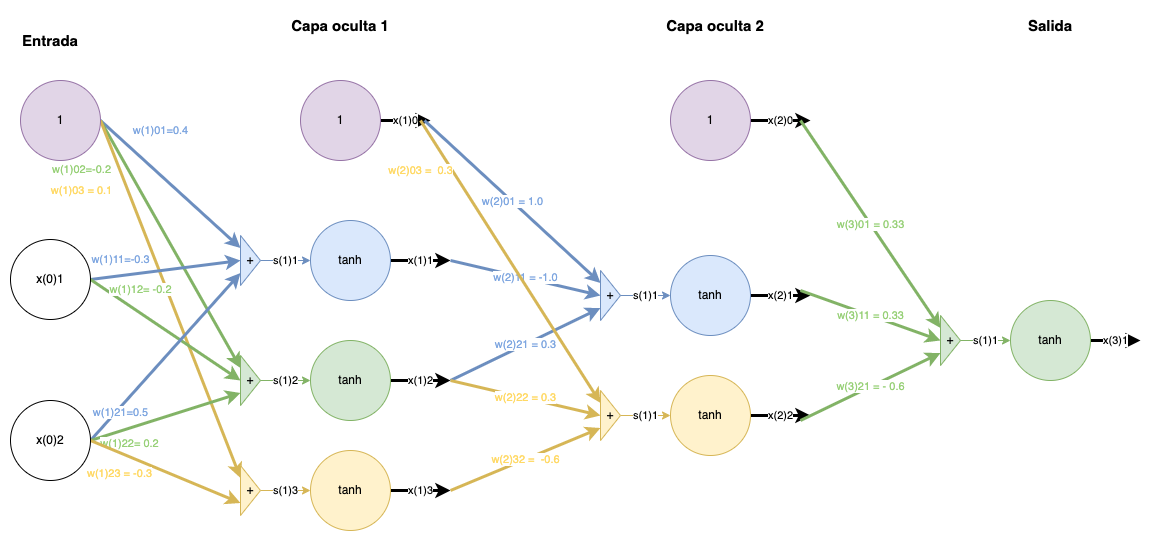
\includegraphics[width=\textwidth]{introduccion_redes_neuronales/construccion_redes_neuronales/rrnn-2-3-2-1-completa.png}
    \caption{Ejemplo de red neuronal con tres capas ocultas}
    \label{img:construccion_rrnn:rrnn-2-3-2-1}
\end{figure} 
Está compuesta por tres capas ocultas, el vector de entrada $x \in \R^2$, 
la primera capa oculta está compuesta por tres neuronas, la segunda por dos y la última, la salida por una. 
Las \textit{flechas} que conectan los nodos hacen referencia a los pesos de cada red neuronal. Por lo que para nosotros 
\begin{align}
    W^{(1)} = 
    \begin{bmatrix}
        0.4 & -0.3 & 0.5\\
        -0.2 & -0.2 & 0.2\\
        0.1 & 0 & -0.3
    \end{bmatrix} ,
    W^{(2)} = 
    \begin{bmatrix}
        1 & -1 & 0.3 & 0\\
        0.3& 0 & 0.3 & -0.6 
    \end{bmatrix} ,
    W^{(3)} = 
    \begin{bmatrix}
        0.33 & 0.33 & -0.6 \
    \end{bmatrix} 
\end{align}
Y si hacemos $x_0 = (1,0)$ y tomamos como función de activación
a la tangente hiperbólica, la ejecución del algoritmo queda reflejada en la tabla \ref{tab:construcción_rnnn:ejemplo_forward_propagation} resultando que 
$h((1,0)) = 0.439$.
\begin{table}[H]
    \begin{center}
\begin{tabular}{| c | c | c | c| }
    \hline
    Valor de $l$ &  $W^{(l)}$ & $\bigl(s^{(l)}\bigr)^T $ & $\bigl(x^{(l)}\bigr)^T$ \\ \hline
    0 & & & $(1,0)$ 
    \\ \hline
    1 & 
    $\begin{bmatrix}
        0.4 & -0.3 & 0.5\\
        -0.2 & -0.2 & 0.2\\
        0.1 & 0 & -0.3
    \end{bmatrix}$ 
    & $(0.1, -0.4, 0.1)$ & $(0.1, -0.38, 0.1)$
     \\ \hline
    2 & $\begin{bmatrix}
        1 & -1 & 0.3 & 0\\
        0.3& 0 & 0.3 & -0.6 
    \end{bmatrix}$
    & $(0.786, 0.126)$
    & $(0.656, 0.126)$
    \\ \hline
    3 & $\begin{bmatrix}
        0.33 & 0.33 & -0.6 
    \end{bmatrix}$ 
    & $(0.471)$ 
    & $(0.439)$
    \\ \hline
\end{tabular}
\caption{Ejemplo de ejecución del algoritmo de \textit{forward propagation}}
\label{tab:construcción_rnnn:ejemplo_forward_propagation}
\end{center}
\end{table}

\subsection{\textit{Backpropagation}}

Los parámetros que determinan una red neuronal son sus pesos, 
para actualizarlos utilizaremos la técnica de gradiente descendente. 
Que como ya explicamos consistía en \textit{avanzar} en dirección contraria a la del gradiente. 
\begin{equation}
    W(t+1) = w(t) - \eta \nabla E_{in}(w(t)). 
\end{equation}

Además, con el fin de reducir el coste del cálculo del gradiente, 
se utiliza el algoritmo conocido como \textit{backpropagation} que fue publicado en 
1989 en el artículo \cite{backpropagation-Hinton}. 

Sea $E_{in}(w)$ la función de error, la cual tomaremos como el error dentro de conjunto de entrenamiento, esto es,  si el conjunto 
de entrenamiento está constituido por $N$ datos de la forma $(x_n, y_n)$ con $x_n$ el vector de entrada y $y_n$ el estado o valor deseado para cualquier $n\in \{1, \ldots, N\}.$
\begin{equation}
    E_{in}(w) = \frac{1}{2} \sum^N_{n=1} e_n. 
\end{equation}
Para el cual 
\begin{equation}
    e_n = (h_w(x)- y_n)^2, 
\end{equation}
es una métrica para medir error entre, en nuestro caso  
la red neuronal $h_w$ y los valores deseados, con $w$ el vector que contiene las respectivas matrices de pesos de cada capa 
$W^{(l)} l \in \{1, \ldots, L\}.$  
%% Ejemplo 
Mostraremos un ejemplo primero antes de presentar el método general para facilitar la comprensión del algoritmo. 
% Imagen red neuronal simple
\begin{figure}[h!]
    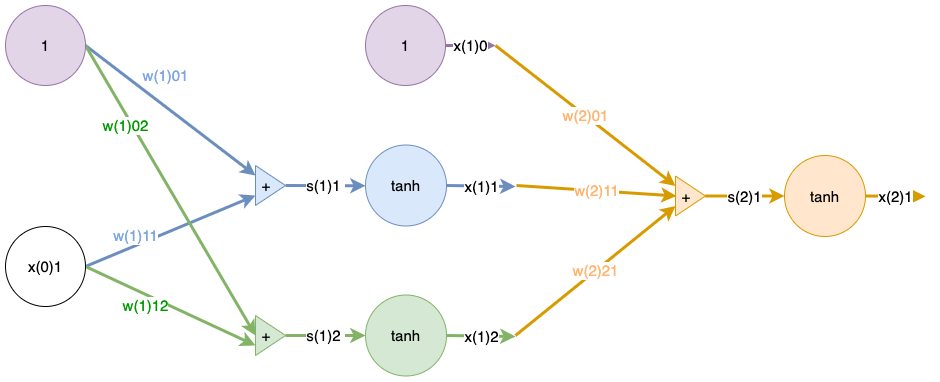
\includegraphics[width=\textwidth]{introduccion_redes_neuronales/construccion_redes_neuronales/rrnn-1-2-1.drawio.png}
    \caption{Ejemplo de red neuronal con tres capas ocultas}
    \label{img:construccion_rrnn:rrnn-1-2-1}
\end{figure} 
Queremos actualizar los pesos $w$ de la red neuronal 
$f_w : \R \longrightarrow \R$ presentada en \ref{img:construccion_rrnn:rrnn-1-2-1}.
$f_w$ está compuesta de dos capas ocultas. Supongamos que nos basaremos en un dato 
$(x, y)$ así pues podemos suponer que 
\begin{equation}
    E_{in}(w) = \frac{1}{2}e(f_w(x), y) = \frac{1}{2} (f_w(x)- y)^2.
\end{equation}
Como queremos actualizar los pesos utilizando el método de gradiente descendente necesitamos calcular el gradiente $\nabla E_{in}(w)$. 
En nuestro caso, $w=\{W^{(1)}, W^{(2)}\}$ con 
\begin{align}
    W^{(1)} = 
    \begin{bmatrix}
        w^{(1)}_{01} & w^{(1)}_{11} \\
        w^{(1)}_{02} & w^{(1)}_{12} \\
    \end{bmatrix} 
    \text{ y }
    W^{(2)} = 
    \begin{bmatrix}
        w^{(2)}_{01} & w^{(2)}_{11} & w^{(2)}_{21}\\
    \end{bmatrix}. 
\end{align}
Luego 
\begin{equation}
    \nabla E_{in}(w) = 
    \left(
        % primera capa 
        \frac{\partial e}{\partial w^{(1)}_{01}},
        \frac{\partial e}{\partial w^{(1)}_{11}},
        \frac{\partial e}{\partial w^{(1)}_{02}},
        \frac{\partial e}{\partial w^{(1)}_{12}},
        % segunda capa
        \frac{\partial e}{\partial w^{(2)}_{01}},
        \frac{\partial e}{\partial w^{(2)}_{11}},
        \frac{\partial e}{\partial w^{(2)}_{21}}
    \right).
\end{equation} 
Cada parcial se calcula, utilizando la regla de la cadena como
\begin{align}
    \frac{\partial e}{\partial w^{(1)}_{01}} 
    &=
    \frac{\partial e}{\partial s_1^{2}}
    \frac{\partial s_1^{2}}{\partial w^{(1)}_{01}} 
    \\
    &= 
    \frac{\partial }{\partial w^{(1)}_{01}}
         \tanh \left(s^{(2)}_{1}\right)
    \\
    &= 
    \left(1- \tanh^2 \left(s^{(2)}_{1}\right)\right) 
    \frac{\partial s^{(1)}_{1}}{\partial w^{(1)}_{01}}
    \\
    &= 
    \left(1- \tanh^2 \left(s^{(2)}_{1}\right)\right) 
    \frac{\partial }{\partial w^{(1)}_{01}}
    \left(w^{(2)}x^{(1)}\right)
    \\
    &= 
    \left(1- \tanh^2 \left(s^{(2)}_{1}\right)\right) 
    \frac{\partial }{\partial w^{(1)}_{01}}
    \left(
        \sum^2_{i=0}
        w^{(2)}_{i1}x^{(1)}_i
    \right)
    \\
    &= 
    \left(1- \tanh^2 \left(s^{(2)}_{1}\right)\right) 
    \left(
        \sum^2_{i=0}
        w^{(2)}_{i1}\frac{\partial x^{(1)}_i }{\partial w^{(1)}_{01}}
    \right)
    \\
    &= 
    \left(1- \tanh^2 \left(s^{(2)}_{1}\right)\right) 
    \left(
        \sum^2_{i=1}
        w^{(2)}_{i1}\frac{\partial }{\partial w^{(1)}_{01}}
        \left(
            \tanh \left(s^{(1)}_{i}\right)
        \right)
    \right)
    \\
    &= 
    \left(1- \tanh^2 \left(s^{(2)}_{1}\right)\right) 
    \left(
        \sum^2_{i=1}
        w^{(2)}_{i1}
        \left(
            \left(1- \tanh^2 \left(s^{(1)}_{i}\right)\right)
            \frac{\partial  }{\partial w^{(1)}_{01}}
            \left(
                \sum^1_{j=0}\sum^2_{k=1}
                w^{(1)}_{j k}x^{(0)}_j
            \right)
        \right)
    \right)
    \\
    &= 
    \left(1- \tanh^2 \left(s^{(2)}_{1}\right)\right) 
    \left(
        \sum^2_{i=1}
        w^{(2)}_{i1}
        \left(
            \left(1- \tanh^2 \left(s^{(1)}_{i}\right)\right)
            x^{(0)}_0
        \right)
    \right).
\end{align}
Notemos que no se han evaluado las apariciones de $s_i^{(j)}$.
Otro ejemplo sería
\begin{align}
    \frac{\partial e}{\partial w^{(2)}_{21}} 
    &=
    \frac{\partial }{\partial w^{(2)}_{21}}
         \tanh \left(s^{(2)}_{1}\right)
    \\
    &= 
    \frac{\partial }{\partial w^{(2)}_{21}}
         \tanh \left(w^{(2)}x^{(1)}\right)
    \\
    &= \left(
    1- \tanh^2 \left(s^{(2)}_{1}\right) \right)x^{(1)}_2.
\end{align}

Notemos que no se han desarrolla los términos de la forma $s^{(i)}_j$. Además si existen $Q$ pesos la complejidad del cálculo será $\mathcal{O}(Q^2)$, sin embargo, como hemos visto existen términos que se repiten en ambas ecuaciones, luego utilizando técnicas de 
programación dinámica y almacenando los valores que se repiten, 
reduciremos el coste a una complejidad de $\mathcal{O}(Q).$ Este 
algoritmo se le conoce como el de \textit{backpropagation}
basaremos su explicación en la publicada en
el artículo \cite{backpropagation-Hinton}.
%% Fin del ejemplo 
%% COMIENZA EL ARTÍCULO 

%Formalizaremos primero qué parámetros debemos estimar del gradiente.

Sea $\theta$ una función de activación derivable, 
 $L$ el número de capas ocultas, $N$ el tamaño del conjunto de entrenamiento $x^{(0)} = (1, x_1, \ldots, x_{d^{(0)}})^T$ 
siendo $x = (x_1, \ldots, x_{d^{(0)}})^T$ la entrada de la red neuronal, $x^{(L)}$ la salida de la red neuronal y 
$d^{(l)}$ la dimensión, número de nodos en la capa $l$-ésima. 
Recordemos que 
para cualquier $l \in \{1, \ldots, L\}$ con
\begin{equation}
    x^{(l)}
     = 
     \theta \left( s^{(l)}\right) 
     = 
     \theta \left( W^{(l)} x^{(l-1)}\right),
\end{equation}
y
\begin{equation}
    E(w) = \frac{1}{2} 
    \sum_{n = 1}^{N}
    \sum_{i = 1}^{d^{(L)}}
    \left({x_n}^{(L)}_i-y_{n_i} \right)^2
\end{equation}

%% Gradiente de la salida: 
Para simplificar la notación renombramos 
\begin{equation}
    E(w) = \sum^{N}_{n=1} e_n.
\end{equation}
y de ahora en adelante nos referiremos como $e$ a $e_n.$
Vamos a proceder a calcular primero los gradientes de la última capa, 
sea $w^{(L)}_{i j}$  con $j \in \{1, \ldots , d^{(L)}\}$, 
$i \in \{1, \ldots , d^{(L-1)}\}$  el peso que relaciona la salida 
$x_i ^{(L-1)}$ del  
nodo $i$ de la capa anterior con la entrada $s_j ^{(L)}$ del nodo $j$ de la última capa. 
Vamos a calcular $\frac{\partial e}{ w^{(L)}_{i j}}$ utilizando la regla de la cadena. 
\begin{equation}
    \frac{\partial{e}}{\partial w^{(L)}_{i j}}
     = 
     \frac{\partial{e}}{\partial x^{(L)}_j} 
     \frac{\partial x^{(L)}_j}{\partial s^{(L)}_j} 
     \frac{\partial s^{(L)}_j}{\partial w^{(L)}_{i j}}.
\end{equation}
Donde es fácil ver que para el tercer término
\begin{equation}\label{eq:backpropagation_s_última_capa_derivada}
    \frac{\partial s^{(L)}_{j}}{\partial w^{(L)}_{i j}}
    = 
    \frac{\partial }{\partial w^{(L)}_{i j}}
    \left(
        w^{(L)}_{\ast j } \cdot x^{(L-1)}
    \right)
    = 
    x^{(L-1)}_j
\end{equation}
Donde $w^{(L)}_{\ast j} = \left(w^{(L)}_{0 j}, w^{(L)}_{2 j}, \ldots, w^{(L)}_{d^{(L-1)} j}\right)$ representa los pesos correspondientes al nodo $j$,
 en forma de  vector fila y $x^{(L-1)} = \left(1, x ^{(L-1)}_1, \ldots, x ^{(L-1)}_{d^{(l-1)}}\right)^T$ el valor de la salida de la capa $L-1$
 en forma de vector columna.
 
 Por otro lado 
 \begin{equation}\label{eq:backpropagation_E_última_capa_derivada}
    \frac{\partial{e}}{\partial x^{(L)}_j} =
    x^{(L)}_j - y_j
 \end{equation}
 donde conocemos $x^{(L)}_j$ gracias al algoritmo de \textit{forward propagation}
 y $y_j$ la componente $j$-ésima del vector deseado en el entrenamiento.
y finalmente
\begin{equation}\label{eq:backpropagation_x_última_capa_derivada}
    \frac{\partial x^{(L)}_j}{\partial s^{(L)}_j} 
    = 
    \frac{d}{d s^{(L)}_j} 
        \theta \left( 
            s^{(L)}_j
        \right)
\end{equation}
que sabemos que se puede calcular por ser $\theta$ derivable y 
$s^{(L)}_j$ un valor conocido que ya ha sido calculado por el algoritmo de 
\textit{forward propagation.}

Por lo tanto, concluimos por 
(\refeq{eq:backpropagation_E_última_capa_derivada}),
(\refeq{eq:backpropagation_x_última_capa_derivada})
y  
(\refeq{eq:backpropagation_s_última_capa_derivada})
\begin{equation}
    \frac{\partial{e}}{\partial w^{(L)}_{i j}}
     = 
     \frac{\partial{e}}{\partial x^{(L)}_j} 
     \frac{\partial x^{(L)}_j}{\partial s^{(L)}_j} 
     \frac{\partial s^{(L)}_j}{\partial w^{(L)}_{i j}} 
    =
    \left( x^{(L)}_j - y_j \right) 
    \theta' \left( s^{(L)}_j\right)
    x^{(L)}_j.
\end{equation}
%%%% Gradiente interior 
Denotaremos por \textit{sensibilidad} a 
\begin{equation}
    \delta^{(l)} = \frac{\partial e}{ \partial s^{(l)}}.
\end{equation}

Para calcular la derivada de pesos de capas interiores 
$l \in \{1 \ldots L-1\}$
procederemos de la siguiente manera, para 
$j \in \{1, \ldots , d^{(l)}\}$ y 
$i \in \{1, \ldots , d^{(l-1)}\}$ 
\begin{equation}
    \frac{\partial{e}}{\partial w^{(l)}_{i j}}
     = 
     \frac{\partial e}{\partial s^{(l)}_j} 
     \frac{\partial s^{(l)}_j}{\partial w^{(l)}_{i j}}
    = 
    \delta^{(l)}
    \frac{\partial}{\partial w^{(l)}_{i j}}
    w^{(l) \cdot x^{(l-1)}}
    = 
    \delta^{(l)} x^{(l-1)}_i,
\end{equation}
donde  $x^{(l-1)}_i$ es conocida por el algoritmo de 
$\textit{forward propagation}$. por otra parte $\delta^{(l)}$ 
cumple que 
\begin{align}
    \delta^{(l)} 
    &= 
    \frac{\partial e}{\partial s^{(l)}}
    \\
    &= 
        \frac{\partial e}{\partial s^{(l+1)}}
        \frac{\partial s^{(l+1)}}{\partial s^{(l)}}
    \\
    &= 
    \delta^{(l+1)} 
    \otimes 
    \frac{\partial}{\partial s^{(l)}}
        \left( w^{(l)} \cdot \theta(s^{(l)})\right)
    \\
    &= 
    \delta^{(l+1)} 
    \otimes 
    w^{(l)} \cdot \theta'(s^{(l)}). 
\end{align}
\textcolor{red}{ Revisar penúltima operación.}
De esta manera a partir de las \textit{sensibilidades} de las 
capas posteriores es posible calcular las $l$-ésimas y puesto que 
la sensibilidad $\delta_{(L)}$ es conocida acabamos de determinar 
cómo calcular la derivada de todos los pesos  de manera constructiva. 
Procedemos a explicitar los cálculos. 

\subsubsection*{Algoritmo}  

El razonamiento expuesto conduce al siguiente proceso algorítmico 
para el cálculo de los gradientes. 
% pseudo código cálculo de sensibilidades 
\begin{algorithm}
    \caption{Algoritmo \textit{backpropagation} para calcular
    las sensinilidades $\delta^{(l)}$}
    \hspace*{\algorithmicindent} \textbf{Input}: un par de $(x,y)$ del conjunto de entrenamiento.  \\
    \hspace*{\algorithmicindent} \textbf{Output} 
    \begin{algorithmic}[1]
        % Forward propagation
        \STATE Se ejecuta el algoritmo de \textit{forward propagation} 
        
        con $x$ como entrada para calcular y guardar : 
        \begin{align}
            s^{(l)} \quad &\text{for } l = 1, \ldots, L;
            \\
            x^{(l)} \quad &\text{for } 0 = 1, \ldots, L;
        \end{align}
        % Inicializamos
        \STATE \COMMENT{Inicializamos sensibilidades últimas capas}
        \begin{equation}
            \delta^{(L)} \longleftarrow 2
            \left( 
                x^{(L)} - y
            \right)
            \theta' \left( s^{(L)} \right)
        \end{equation}
        \STATE 
        \COMMENT{ \textit{Backpropagation}}
        
        \For{$l = L-1$ to $1$}
        {
            \begin{equation}
                \delta^{(l)} 
                    \leftarrow
                \theta' 
                \left(
                    s^{(l)}
                \right)
                \otimes
                \left[
                    W^{(l+1)}
                    \delta^{(l+1)}
                \right]^{d^{(l)}}_1
            \end{equation}
        }
\end{algorithmic}
\end{algorithm}

% Las redes neuronales multicapa son aproximadores universales 
% !TeX root = ../../tfg.tex
% !TeX encoding = utf8
%
%*******************************************************
% Introducción artículo MFNAUA
%*******************************************************
\section{Las redes neuronales son aproximadores universales}  

Tras las definición \ref{sec:redes-neuronales-intro-una-capa} de red neuronal expuesta,
es pertinente la pregunta si tal estructura será 
capaz de aproximar con éxito una función genérica desconocida.   

Aunque las redes neuronales multicapa ya se venían aplicando con anterioridad, 
véase por ejemplo los usos expuestos durante la primera conferencia
internacional de redes neuronales de \cite{4307059} de 1987, 
no fue hasta 1989 que se descubrió formalmente su alcance.
 Tal delimitación se propuso en el artículo 
\textbf{Multilayer Feedforward Networks are Universal Approximators} \cite{HORNIK1989359}
 escrito por Kurt Hornik, Maxwell Stinchcombe y Halber White enunciando: 

\begin{teorema}\textbf{Las redes \textit{feedforward} multicapa son una clase de aproximadores universales } \label{teo:MFNAUA}
    \\
    Una red neuronal \textit{feedforward} multicapa estándar con tan solo una capa oculta y con una función de activación cualquiera es capaz de aproximar cualquier 
    función Borel medible  con dominios y codominios de dimensión finita (no necesariamente iguales) y con el nivel de precisión que se desee siempre y cuando 
    se utilicen suficientes neuronas. En este sentido las redes \textit{feedforward} multicapa son una clase de aproximadores universales.

\end{teorema}

En las secciones siguientes, con el fin de alcanzar una
 comprensión profunda de las redes neuronales,
trataremos de desgranar y profundizar en el artículo y su 
demostración. Primero precisaremos o introduciremos conceptos elementales 
sobre redes neuronales \ref{ch:articulo:sec:defincionesPrimeras}, después 
demostraremos el teorema en el caso real 
\ref{teo:TeoremaConvergenciaRealEnCompactosDefinicionesEsenciales} e iremos refinando y generalizando los resultados hasta probar
el resultado enunciado \ref{teo:MFNAUA} para una capa oculta.

 % Nota margen de denso
 \setlength{\marginparwidth}{\bigMarginSize}
 \marginpar{\maginLetterSize
     \iconoAclaraciones \textcolor{dark_green}{ 
         \textbf{Idea intuitiva conjunto denso.}
     }
     Si $S$ es denso en $T$, 
     se está está diciendo que \textbf{los elementos de $S$ son capaces de aproximar cualquier elemento de $T$
     con la precisión que se desee}. 
 }

 
El esquema general será: 

\begin{align*}
    \rrnn 
        \xRightarrow[]{\ref{teo:2_4_rrnn_densas_M}}  
    \rrnng 
        \xRightarrow[]{\ref{teorema:2_3_uniformemente_denso_compactos}}
    \pmcg
        \xRightarrow[]{\ref{teo:TeoremaConvergenciaRealEnCompactosDefinicionesEsenciales}}     
    \fC    
        \xRightarrow[]{\ref{teo:2_2_denso_función_continua}} 
    \fM.
\end{align*}

   

\begin{itemize}
    \item Las redes neuronales que nosotros hemos modelizado son densas en un espacio más general que hemos denominado \textit{Anillo de aproximación de redes neuronales}
    generado a partir de una función de activación $\psi$. 
    \item Que a su vez es denso en el \textit{Anillo de aproximación de redes neuronales}
    generado a partir de una función medible $G$. 
    \item El espacio \textit{Anillo de aproximación de redes neuronales} es denso en el de las funciones continuas.
    \item Las funciones continuas son densas en el espacio de funciones medibles. 
\end{itemize}

Si quisiéramos situar en este esquema a otras definiciones de redes neuronales las situaríamos entre  nuestro modelo y el espacio \textit{Anillo de aproximación de redes neuronales}; en  el capítulo \ref{chapter:construir-redes-neuronales} se probará tal resultado y analizarán los beneficios de basarnos en un modelo más simple. 



% !TeX root = ../../tfg.tex
% !TeX encoding = utf8
%
%*******************************************************
% Contenido del artículo 1: Definiciones primeras
%*******************************************************

\section{Definiciones primeras}\label{ch:articulo:sec:defincionesPrimeras}  

Comenzaremos presentando definiciones básicas sobre redes neuronales. 


\begin{definicion}[Función de activación] \label{def:funcion_activacion_articulo}
    Una función  $\psi: \R \longrightarrow [0,1]$ es una \textbf{ función de activación} si  cumple las siguientes propiedades:
    \begin{enumerate}[label=(\roman*)]
        \item Es no decreciente.
        \item $\lim _{x \rightarrow \infty} \psi(x) = 1
        $.
        \item $\lim _{x \rightarrow -\infty} \psi(x) = 0$.
    \end{enumerate}  
   
    Ejemplos comunes de funciones de activación son

    %%% Nota sobre funciones activación más democráticas que otras
    \marginpar{\maginLetterSize
         \iconoProfundizar \textcolor{blue}{    
        \textbf{Observación sobre la idoneidad de cada función activación:}
    }
    Se probará la convergencia de las redes neuronales independientemente de la función de activación seleccionada. Cabe entonces la pregunta
    ¿Existen funciones de activación más democráticas que otras? 
    Se discutirá esta pregunta en \ref{funciones-activacion-democraticas-mas-demoscraticas}.
    }

    % Imágenes de la función indicadora 
    \begin{figure}[h]
        \centering
        \begin{subfigure}[t]{0.47\textwidth}
            \centering
            \includegraphics[width=\textwidth]{
                articulo_rrnn_aproximadores_universales/función_indicadora_l_0.png}
            \caption{Función indicadora $\lambda_0 = 0$}  
            \label{fig:función_indicadora}
        \end{subfigure}
        \hfill
        \begin{subfigure}[t]{0.47\textwidth}  
            \centering 
            \includegraphics[width=\textwidth]{articulo_rrnn_aproximadores_universales/función_umbral_lineal.png
            }
            \caption{Función umbral $w=(2)$, $t=1$}    
            \label{fig:función_umbral_lineal}
        \end{subfigure}
        \begin{subfigure}[t]{0.47\textwidth}   
            \centering 
            \includegraphics[width=\textwidth]{articulo_rrnn_aproximadores_universales/función_rampa.png}
            \caption{Función rampa} 
            \label{fig:funciones_rampa}
        \end{subfigure}
        \hfill
        \begin{subfigure}[t]{0.47\textwidth}   
            \centering 
            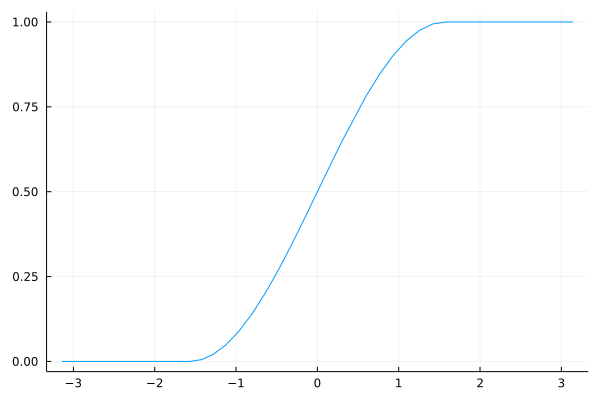
\includegraphics[width=\textwidth]{articulo_rrnn_aproximadores_universales/cosineSquasherSinTitulo.png}
            \caption{\textit{Cosine Squasher}}   
            \label{fig:cosine_squasher}
        \end{subfigure}
        \caption{Ejemplos de funciones de activación} 
        \label{fig:EjemplosFunciónActivación}
    \end{figure}

    \begin{itemize}
        \item \textbf{Funciones indicadoras} \ref{fig:función_indicadora}: $\psi(\lambda) = 1_{\{\lambda > \lambda_0\}}$ con $\lambda_0 \in \R$. 
        
        \item \textbf{Funciones umbral} \ref{fig:función_umbral_lineal}:
        Una función umbral, es una función booleana monótona $\psi_w: \{0,1\}^n \longrightarrow \{0,1\},$ 
        donde para $w \in \R^n$, $t \in \R$ fijos se
        satisface que 
        \begin{equation}
            \psi_w(x) = \left\{
                \begin{array}{lcc}
                    1, &   si  & w \cdot x \geq t \\
                    0, &  si & w \cdot x < t.\\
                    \end{array}
            \right.
        \end{equation}
        
        \item \textbf{Función rampa} \ref{fig:funciones_rampa}: $\psi(\lambda)  = \lambda 1_{\{0 \leq \lambda \leq  1\}} + 1_{\{\lambda > 1\}}.$
    
        \item \textbf{La función \textit{cosine squasher}} de Gallant and White 
        \ref{fig:cosine_squasher} (1988) \cite{Gallant88thereexists}. 
        \begin{equation*}
    \psi(\lambda )= \left(1 + \cos\left(\lambda + 3 \frac{\pi}{2} \right) \frac{1}{2}\right) 
     1_{\{\frac{-\pi}{2} \leq \lambda \leq  \frac{\pi}{2}\}}
     +
     1_{\{ \frac{\pi}{2} < \lambda \}}.
    \end{equation*}
    \end{itemize}

   Notemos que así definidas las funciones de activación son medibles, ya que la imagen inversa de un abierto de $[0,1]$ siempre será un conjunto medible de  $\R$  (capítulo 7  página 77 \cite{nla.cat-vn1819421}).
    

    Cabe destacar que la definición tomada es la propuesta en \cite{HORNIK1989359} y que existen
    otras posibles definiciones menos restrictivas con las que también se ha probado la convergencia universal.
    Por ejemplo podrían aceptarse funciones de activación no continuas (véase \cite{FUNAHASHI1989183}); 
    o como 
    se demuestra en \cite{DBLP:journals/corr/SonodaM15} y en \cite{non-polynomial-activation-functions}, funciones de activación no polinómicas y no acotadas. 
\end{definicion}

% Nota sobre que la funciones de activación 
% son clave en el aprendizaje
\setlength{\marginparwidth}{\smallMarginSize}
\marginpar{\maginLetterSize
    \iconoClave  \textcolor{darkRed}{     
        \textbf{
            Las funciones de activación $\Gamma$ son la clave del aprendizaje
        }
    }
    \label{ch03:funcionamiento-intuitivo-funcion-activacion}

La idea intuitiva es que cada neurona 
lo que se hace es \textit{colocar} por transformaciones afines la imagen de la función de activación en el espacio con el fin 
de aproximar una región de la imagen de la función ideal. 
Por lo tanto, la forma que ésta tenga será determinante en el número de neuronas necesarias para la convergencia.    
}
\setlength{\marginparwidth}{\bigMarginSize}

% Fin del tratamiento de funciones de activación 

Para cualquier natural $d$ mayor que cero  denotaremos por $\afines$ al conjunto de todas 
las \textbf{funciones afines} de $\R^d$ a $\R$. Es decir el conjunto de funciones de la forma 
$A(x) = w \cdot x + b$ donde $x$ y $w$ son vectores de $\R^d$,  $b \in \R$ es un escalar
 y $\cdot$ representa el producto escalar
usual. En este contexto, $x$ corresponde al vector entrada de la red neuronal, $w$ los pesos de la red
que se multiplicarán con $x$ en la capa intermedia y $b$ el sesgo. 

   % Nota margen sobre que abstrae esta estructura de red neuronal
 \marginpar{\maginLetterSize
 \iconoAclaraciones \textcolor{dark_green}{     
 \textbf{Idea tras la definición de $\pmc$.}
 }
Nótese que de acorde a la definición  \ref{definition:redes_neuronales_una_capa_oculta}
lo que se está refiriendo es la clase de las redes 
neuronales de una capa oculta y \textbf{salida de una dimensión}.
Donde cada sumando representa una neurona de la capa oculta.
}
%%% fin nota
\begin{definicion} [Formalización de una red neuronal de una capa oculta y salida real]
    Para cualquier función Borel medible $G$, definida de $\R$ a $\R$ y cualquier natural positivo
    $d \in \N$ se define a la clase de funciones $\pmc$ como 

    \begin{equation}
        \begin{split}
        \pmc = 
        \{ 
            & f: \R ^d \longrightarrow \R / \quad
            f(x)=\sum_{j = 1} ^q (
            \beta_j G(A_{j}(x))), \\
            & x  \in \R ^d, \beta_j \in \R, A_{j}\in \afines,q \in \N
        \}.
        \end{split}
    \end{equation}

    Conforme avancen los resultados teóricos veremos que $\pmc$ 
    no depende de la función $G$ seleccionada; así pues, tras enunciar tales resultados nos referiremos sin ambigüedad a tal conjunto como $\rrnn$.
\end{definicion}


Definiremos a continuación una familia de funciones más generales que $\pmc$ con la intención de que actúe como nexo de unión entre la clase de funciones continuas y las redes neuronales de una capa facilitándonos con ello la prueba de los resultados. La familia que introduciremos solo tiene 
una utilidad teórica, es decir no tendrá ninguna relevancia a nivel práctico en cuanto a implementaciones.
   
% Nota margen sobre Idea intuitiva de la definición 
\marginpar{\maginLetterSize
\iconoAclaraciones \textcolor{dark_green}{     
\textbf{Motivación de la definición de $\pmcg$}}.

En un principio será más fácil demostrar que con 
funciones de esta clase seremos capaz de aproximar cualquier función continua.
De esta manera este conjunto actuará de nexo de unión entre las funciones continuas y las redes neuronales 
facilitando las demostraciones. De ahora en adelante nos
 referiremos a este conjunto como al \textbf{de anillo de aproximación} (como curiosidad, el nombre proviene a que
  tiene estructura de anillo y que se utilizará para 
  aproximar funciones continuas).
}
\begin{definicion} [Anillo de aproximación de redes neuronales]\label{def:articulo_abstracción_rrnn}
    
    \begin{equation} 
        \begin{split}
        \sum \prod^d(G) = \{ 
        &f: \R^r \longrightarrow \R / \quad
        f(x) = \sum_{j = 1} ^q  \beta_j \prod_{k=1}^{l_j}
        G(A_{jk}(x)), \\
        &x  \in \R^d, \beta_j \in \R, A_{jk}\in \afines; l_j,q \in \N
        \}.
    \end{split}
    \end{equation}  

 
    Notemos que $\pmc$ se recupera en el caso particular en el que $l_j = 1$ para todo $j$.
    Los elementos de $\pmcg$ son combinaciones lineales de productos finitos de neuronas. 

\end{definicion}

\reversemarginpar
  %%% Nota margen sobre función medible 
  \setlength{\marginparwidth}{\smallMarginSize}
  \marginpar{\maginLetterSize
    \iconoAclaraciones \textcolor{dark_green}{     
        \textbf{
            Aplicación práctica aprendizaje automático y 
            relación con las funciones medible.
        }
    }
    \textbf{A nivel práctico se tiene un conjunto de datos
    para los cuales queremos extraer un patrón} que nos permita 
    predecir la naturaleza de datos nuevos. Es por ello necesario
    suponer que estos datos están regidos por alguna regla, la cual 
    puede ser todo lo extraña posible pero que toma valores 
    que pueden ser observables y cuantificables en la mayoría de los casos, estos comportamientos son formalizados
     matemáticamente con \textbf{funciones medibles}.
}
\setlength{\marginparwidth}{\bigMarginSize}
\normalmarginpar 

Introducimos a continuación la notación de los conjuntos de funciones que seremos capaces de aproximar.  

Denotamos por  $\fC$ al conjunto de funciones continuas con dominio en $\R^d$ y codominio $\R$,
por  $\fM$ al conjunto de todas las funciones Borel medibles de $\R^d$ a $\R$; 
y por $B^d$ a la $\sigma$-álgebra de Borel en $\R ^d$. 

En lo que respecta a definiciones anteriores, $\pmc$ y $\pmcg$ están contenidos en
$\fM$ para cualquier función Borel-medible $G$. Si $G$ es continua entonces 
$\pmc$ y $\pmcg$ pertenecen a $\fC$. Tengamos presente que $\fC$ es un subconjunto
de $\fM$.  

De ahora en adelante nos referiremos a Borel-medible como medible. 
  

\subsection{ Reflexión sobre el tipo de funciones que se pueden aproximar}

La existencia de funciones no medibles manifiesta una limitación
de la formalización actual de las redes neuronales que plantea las siguientes 
preguntas: 
\begin{enumerate}
    \item ¿Supone la existencia de este tipo de funciones una verdadera limitación a nivel práctico?
    \item ¿Se podría construir alguna arquitectura que sí que las aproximara?
\end{enumerate}  

Continuando con el hilo de la segunda cuestión, si se carece de un espacio vectorial, 
de una medida,  ¿Cómo se podría construir una sucesión de funciones que se aproxime?
Quizás habría que buscar características más intrínsecas del problema en cuestión, 
razonamientos topológicos.

\begin{definicion} [Subconjunto denso]
    % Nota margen de denso
    \reversemarginpar 
    \marginpar{\maginLetterSize
        \iconoAclaraciones \textcolor{dark_green}{ 
            \textbf{Idea intuitiva conjunto denso.}
        }
        Si $S$ es denso en $T$, 
        se está está diciendo que \textbf{los elementos de $S$ son capaces de aproximar cualquier elemento de $T$
        con la precisión que se desee}. 
    }
    \normalmarginpar

    Dado un subconjunto $S$ de un espacio métrico $(X, \rho)$, se dice que $S$ es denso por la distancia $\rho$
    en subconjunto $T$ si para todo $\varepsilon$ positivo y cualquier $t \in T$ existe un $s \in S$ tal 
    que $\rho(s,t) \leq \varepsilon$. 
\end{definicion}

Un ejemplo habitual es en el espacio métrico $(\R, |\cdot|)$ con $|\cdot|$ el valor absoluto, el subconjunto 
$T = \R$ y $S$ los números irracionales, $S = \R \setminus \Q$. 


\begin{definicion} 
    Un subconjunto $S$ de $\fC$ se dice que es \textbf{uniformemente denso para compactos} en  $\fC$
    si para cada subconjunto compacto $K \subset \R^d$ se tiene que $S_K$ es denso según $\rho_K$ en $\fC$
    donde $\rho_K$ está definida como sigue.
    Para cualquier $f,g \in \fC$ 
    \begin{equation}
        \rho _ K (f,g) = \sup_{x \in K} |f(x) - g(x)|.
    \end{equation}

    % Nota intuitiva de compacto
    \marginpar{\maginLetterSize
        \iconoAclaraciones \textcolor{dark_green}{ 
          \textbf{Noción intuitiva de compacto}
        }

        Un compacto es un conjunto que \textbf{se puede cambiar por un subconjunto finito cometiendo un error prefijado}. 

        Al trabajar con números reales, un espacio es compacto si es cerrado y acotado, lo que a nivel práctico significa que los
        \textbf{datos de entrada se encuentran dentro de un rango concreto}. 
      }

      % Nota intuitiva de uniformemente denso
      \marginpar{\maginLetterSize
        \iconoAclaraciones \textcolor{dark_green}{ 
          \textbf{Noción intuitiva de uniformemente denso para compactos }
        }
          lo que indica es que \textit{controlamos} \textbf{cuánto de cerca
          están dos funciones sea cual sea cualquier punto del compacto en que evaluemos} es decir, podríamos afirmar que para una red neuronal que tome valores por ejemplo en $[0,1]^r$, se puede saber que su error es menor que $\varepsilon \in\R^+$ independientemente de la entrada.
      }
      
\end{definicion}

\begin{definicion}
    Una serie de funciones $\{f_n\}$ \textbf{converge uniformemente a una función $f$ sobre compactos} si para 
    cada  conjunto compacto $K \subset \R^d$  se cumple que
    \begin{equation}
        \rho_k (f_n, f) \longrightarrow 0 \text{ cuando } n \longrightarrow \infty.
    \end{equation} 
\end{definicion}


% !TeX root = ../../tfg.tex
% !TeX encoding = utf8
%
%*******************************************************
% Contenido del artículo 2: Primeros resultados
%*******************************************************


\section{Primeros resultados} 
% Introducción sección 


%%%%% primer teorema de convergencia  
% Teorema 2.1 
\begin{teorema} [Teorema de convergencia real en compactos]  \label{teo:TeoremaConvergenciaRealEnCompactosDefinicionesEsenciales}

    Sea G cualquier función continua no constante definida de $\R$ en $\R$. 
    Se tiene que $\pmcg$ es uniformemente denso para compactos en $\fC$.
\end{teorema}

\begin{proof}
    Bastará probar que el conjunto $\pmcg$ satisface las hipótesis del teorema de
     Stone-Weierstrass \ref{ch:TeoremaStoneWeiertrass}.
    Lo primero será comprobar que $\pmcg$ es un álgebra, para ello veamos que:         
    \begin{enumerate}
        \item La función constante uno pertenece al conjunto. 
        Como $G$ no es constante existirá un valor de la imagen distinto de $0$, supongamos que $G(a)= b \neq 0$ para $a,b \in \R.$
        Consideremos la función afín $A(x) = 0 \cdot x + a$, está claro que $\frac{1}{b}G(A(x))$ es la función constantemente uno. 
        \item El conjunto $\pmcg$ es cerrado para sumas y producto por escalares reales. 
        En efecto, si $f,g$ pertenecen a  $\pmcg$, serán de la forma
         $f = \sum_{j = 1} ^q  \beta_{fj} \prod_{k=1}^{l_{fj}}  G(A_{fjk}(x))$ y 
        $g = \sum_{j = 1} ^p  \beta_{gj} \prod_{k=1}^{l_{gj}}G(A_{gjk}(x))$  por lo que
        \begin{equation}
            \begin{split}
                \gamma f+ \sigma g =& \gamma \sum_{j = 1} ^q  \beta_{fj} \prod_{k=1}^{l_{fj}}  G(A_{fjk}(x)) + 
                \sigma \sum_{j = 1} ^p  \beta_{gj} \ \prod_{k=1}^{l_{gj}}G(A_{gjk}(x)) \\
                & = \sum_{j = 1} ^q  (\gamma \beta_{fj})  \prod_{k=1}^{l_{fj}}  G(A_{fjk}(x)) + 
                \sum_{j = 1} ^p  (\sigma \beta_{gj}) \ \prod_{k=1}^{l_{gj}}G(A_{gjk}(x)).
            \end{split}
        \end{equation}
        
        Basta renumerar una de las sumatorias para ver $\gamma f+ \sigma g$ como una combinación 
        lineal de productos finitos de perceptrones y por tanto $\gamma f+ \sigma g \in \pmcg.$
        
        \item Cerrado para producto. Para $f,g \in \pmcg$, se tiene que $fg$ pertenece a $\pmcg$. 
        Renombrando los índices de la sumatoria con $\Lambda = i\{1..l_i\} \cup j\{1..l_j\}$ basta ver que 
        \begin{equation}
            \begin{split}
                fg &= \left(\sum_{i \in I_f} \beta_{j}  \prod_{k=1}^{l_{i}}  G(A_{ik}(x))\right)
                    \left(\sum_{j \in I_g}   \beta_{j}  \prod_{k=1}^{l_{j}} G(A_{jk}(x)) \right) \\
                    & = \sum_{i \in I_f} \left(  \beta_{j}  \prod_{k=1}^{l_{i}}  G(A_{ik}(x))
                        \left( \sum_{j \in I_g}  \beta_{j} \prod_{k=1}^{l_{j}} G(A_{jk}(x))  \right)  
                     \right) \\
                    & =  \sum_{(i,j) \in I_f \times I_g} (\beta{i}\beta{j}) \prod_{k \in \Lambda} G(A_{k}(x))
            \end{split}
        \end{equation}
        luego $fg \in \pmcg$. 
    \end{enumerate}

    Veamos que $\pmcg$ separa puntos cada compacto $K \subset \R^r$. 

    Por ser $G$ no constante existirán $a,b \in \R$ distintos cumpliendo que $G(a) \neq G(b)$. Fijadas $x,y \in K$ tomamos entonces cualquiera de las 
    funciones afines que cumplen que $A(x) = a$ y $A(y)=b$ 
    \footnote{Sabemos que al menos una habrá, ya que podemos plantear la función afín
    como un sistema de ecuaciones lineales de $r+1$ incógnita y 2 soluciones}, 
    por lo que $G(A(x)) \neq G(A(y))$ y tenemos como buscábamos que $\pmcg$ separa los puntos de $K$. 

    Veamos finalmente que para todo punto de $K$ existe una función de $\pmcg$  en el que la imagen no es nula.  

    Por ser $G$ no constante volvemos a tomar un $a \in \R$ tal que $G(a) \neq 0$ , consideramos ahora la aplicación lineal
    $A(x) = 0 \cdot x + a$ por lo que para todo $x \in K$, $G(A(x)) = G(a) \neq 0$. 

    Como hemos comprobado se verifican todas las hipótesis del teorema de Stone-Weierstrass, con lo que concluimos, como queríamos probar que $\pmcg |_K$ es denso en $C(K). $ 
\end{proof}

\subsection{Observaciones y reflexiones sobre el teorema de convergencia real en compactos}

Con esto lo que acabamos de probar que \textit{feedforward neural networks} con tan solo una capa oculta  son capaces de aproximar cualquier 
función continua en un compacto.  Cabe destacar que a la función $G$, la función de activación,
 solo se le ha pedido como 
hipótesis ser una función continua.     

Además, solo se está demostrando para el caso de una capa oculta, como veremos a continuación  de 
manera intuitiva se explica que sea extrapolable también a redes neuronales 
con varias capas ocultas, sin embargo; esto pone de manifiesto, si se quieren formular nuevos teoremas en el campo de las redes neuronales
multicapas a la necesidad de una definición más abstracta de las mismas. 


Se aportan las siguientes generalizaciones del método. 
%%% Corolarios propios 

Notemos que la función de activación $G$ es única en toda la estructura,
sin embargo es habitual la combinación de éstas en una misma red neuronal (
\cite{DBLP:journals/corr/abs-1811-03378}, 
 \cite{8258768}, 
 \cite{DBLP:journals/corr/SzegedyVISW15}
). 

\begin{corolario}[Pueden combinarse distintas funciones de activación en una misma red neuronal]

    Una misma red neuronal puede estar constituida por una familia de funciones continuas no constantes $\Gamma$, 
    bastará con generalizar $\pmcg$ a $\sum \prod ^r (\Gamma)$ donde 
    \begin{equation}
        \begin{split}
            \sum \prod^r (\Gamma) = \{ 
                &f: \R^r \longrightarrow \R /
                f(x) = \sum_{j = 1} ^q  \beta_j \prod_{k=1}^{l_j}
                G(A_{jk}(x)), \\
                &x  \in \R^r, \beta_j \in \R, A_{jk}\in A^r, l_j,q \in \N, G \in \Gamma
                )
                \}
        \end{split}
    \end{equation}
    Es decir, combinaciones lineales de perceptrones cuyas funciones 
    de activación pueden diferir unas de otras. 
\end{corolario}

\begin{proof}
    La demostración es idéntica a la dada en el Teorema de convergencia 
    real en compactos \ref{teo:TeoremaConvergenciaRealEnCompactosDefinicionesEsenciales}.
\end{proof}

Notemos que este resultado no da pista alguna de las ventajas de una función frente a otra,
 ni cómo afecta a la \textit{velocidad de convergencia}. 

\begin{corolario}[Extensión a múltiples capas ocultas]

    Sea $\Gamma$ cualquier familia de funciones continuas definidas de $\R$ en $\R$. 
    Se tiene que $\sum \prod ^r (\Gamma)$ es uniformemente denso por compactos en $\fC$  
    Es decir, las redes neuronales con varias capas son densas en el  espacio de la funciones continuas de una variable en un compacto. 
\end{corolario}

    Como con una capa ya se nos asegura la convergencia bastará con asegurar que exista 
    en el espacio de las redes neuronales profundas capas que transmitan la información sin cambiarla. 

    Una vez concretada la estructura de la red neuronal,  su estructura algebraica podría permitir esa transmisión. 


Recordemos que de manera general se ha definido $A$ como una función afín 
$A(x) = w \cdot x + b$ donde $x$ y $w$ son vectores de $\R^r$  y $b \in \R$ es un escalar.  ¿Pero que ocurriría si trabajáramos con transformaciones más generales?  
Por ejemplo $B((x_1, ..., x_r)) = \sum_{i= 0} ^N \sum_{j= 0} ^r \alpha_{ij} x_j^i$  con $N$ natural positivo. 

\begin{corolario}[Generalización de A]  
    Se puede extender $A^r$ a conjuntos más generales como el de los polinomios de $r$ variables de grado $N$, $\mathbb{P}$.  
\end{corolario}
\begin{proof}
    Simplemente hay que reparar que $A^r$ está contenido en el espacio $\mathbb{P}$. 
    Es más observando la demostración bastará con utilizar cualquier conjunto que contenga a $A^r$. 
\end{proof}

La utilidad de este corolario a nivel práctico es cuestionable, ya que aumentaría considerablemente el número de 
parámetros que ajustar de la red neuronal ocasionando: (1) la necesidad de mayor número de datos que aprender, 
(2) mayor costo computacional, (3) probablemente peores resultados a igual número de iteraciones en comparativa 
con otros modelos de menor número de neuronas (ya que el espacio de búsqueda ha aumentado).

Podría tener el siguiente interés:
el teorema nos dice que podemos aproximar cualquier función continua de variable real, sin embargo, desconocemos el 
número de neuronas, por capa. Supongamos una situación en la que el número de neuronas esté restringido, en tal caso,
generalizar $A^r$ sí que podría tener un papel importante en cuanto a mejoras. 


%% Definiciones de equivalencia de funciones 
\begin{definicion}[Equivalencia entre funciones]
    Sea $\mu$ una medida de probabilidad en $(\R^r, B^r)$.  Dos funciones 
    $f$ y $g$ pertenecientes a $\fM$, diremos que son $\mu -$equivalentes 
    si $\mu\{ x \in \R^r : f(x)=g(x) \} = 1.$
\end{definicion}

Lo que se está diciendo es que serán iguales casi por doquier.   

% Definición distancia  
\begin{definicion} [Introducción de una distancia basada en una probabilidad]
    Dada una medida de probabilidad $\mu$ en $(\R^r, B^r)$, se define 
    la métrica $\rho_{\mu}$ definida como 
    \begin{equation}
        \begin{split}
            & \rho_{\mu} : \fM \times \fM \longrightarrow \R^+ \\
            & \rho_{\mu}(f,g) = \inf \{ \epsilon > 0: \mu \{ x : |f(x) - g(x)| > \epsilon \} < \epsilon \}.
        \end{split}
    \end{equation}
\end{definicion}  

Con esta definición lo que se está buscando es una forma de decir cuánto 
distan las funciones $f,g$ entre ellas.  

%% Lema 2.1
\begin{lema}[Caracterización de la convergencia de una sucesión]\label{lema:caracterizacionConvergenciaSucesiones2_1}
    Son equivalentes las siguientes afirmaciones: 
    \begin{enumerate}
        \item $\rho_{\mu}(f_n, f) \longrightarrow 0$.
        \item Para cualquier  $\epsilon > 0$ se tiene que $\mu \{  x : |f_n(x) - f(x)| > \epsilon \} \longrightarrow 0$.
        \item $\int \min \{ |f_n(x) - f(x)|, 1\} d\mu(x) \longrightarrow 0.$
    \end{enumerate}
\end{lema}

\begin{proof}
    % 1 -> 2
    Comenzaremos probando (1) $\Rightarrow$ (2). 

    Si $\rho_{\mu}(f_n, f) \longrightarrow 0$
    Fijamos $\epsilon_0 > 0$, tenemos por definición que 
    para cualquier $0 < \delta < \epsilon_0$ existirá $n_0 \in \N$ tal que 
    $\rho_{\mu}(f_n, f) < \delta$ para cada $n$ un natural mayor que $n_0$. Es decir,  
    

    $$\inf \{ \epsilon > 0: \mu \{ x : |f_n(x) - f(x)| > \epsilon \} < \epsilon \} < \delta \quad \forall n \geq n_0$$

    entonces 

    \begin{equation}
        \mu \{ x : |f_n(x) - f(x)| > \epsilon_0 \}
        \leq
        \mu \{ x : |f_n(x) - f(x)| > \delta\}
        < \delta 
        \quad 
        \forall n \geq n_0
    \end{equation}

    lo que significa que 

    \begin{equation}
        \mu \{ x : |f_n(x) - f(x)| > \epsilon_0 \}
        \longrightarrow
        0  
    \end{equation}
    probando con ello la implicación buscada.

    % 2 -> 1
    Veamos ahora que (2) $\Rightarrow$ (1). 
    Fijamos $\epsilon_0 > 0$ y bajo la hipótesis segunda se tiene que 

    \begin{equation}
        \mu \{ x : |f_n(x) - f(x)| > \epsilon_0 \}
        \longrightarrow
        0,  
    \end{equation}
    es decir, que para cualquier real $\delta$ cumpliendo que $0 < \delta < \epsilon_0$ 
    existe un natural $n_0$ a partir del cual todo natural $n$ mayor o igual satisface que 
    
    \begin{equation}
        \mu \{ x : |f_n(x) - f(x)| > \epsilon_0 \}
        \leq
        \mu \{ x : |f_n(x) - f(x)| > \delta\}
        < \delta 
        \quad 
        \forall n \geq n_0
    \end{equation}

    lo que significa que 
    
    \begin{equation}
        \inf \{ \epsilon > 0:
         \mu \{ 
             x : |f_n(x) - f(x)| > \epsilon \} < \epsilon 
             \} 
        < \delta 
        \quad 
        \forall n \geq n_0
    \end{equation}

    que por definición de la distancia equivale a que 

    \begin{equation}
        \rho_{\mu}(f_n, f) < \delta \quad \forall n \geq n_0
    \end{equation}

    probando con ello 

    \begin{equation}
        \rho_{\mu}(f_n, f) \longrightarrow 0. 
    \end{equation}

    % 2 -> 3
    Probaremos ahora que (2) $\Longrightarrow$ (3).   

    Por (2) se tiene que sea cual sea el $\epsilon$ cumpliendo que 
    $0 < \epsilon \leq 2$ 
    existirá un natural $n_0$ a partir del cual, cualquier otro natural $n$ 
    satisface que 
    \begin{equation} 
        \mu \{  
            x : |f_n(x) - f(x)| > \frac{\epsilon}{2}  
            \}  
        < 
        \frac{\epsilon}{2},  
    \end{equation}

    Gracias a esta desigualdad, para cualquier $n > n_0$ podemos acotar la siguiente integral: 

    \begin{equation}
        \int \min \{ |f_n(x) - f(x)|, 1\} d\mu(x) 
        \leq
        \frac{\epsilon}{2} (1-\frac{\epsilon}{2}) + 1\frac{\epsilon}{2} 
         = \epsilon - \frac{\epsilon^2}{4} <  \epsilon.  
    \end{equation}
    probando con ello la implicación (2) $\Longrightarrow$ (3).

    % 3 -> 1
    Finalmente comprobaremos la implicación (3) $\Longrightarrow$ (1).

    Para cada $n\in \N$ llamamos $g_n = \min\{|f_n - f|, 1|\}$.
    Por (2), dado $0 < \epsilon < 1$, existe un $n_0 \in \N$
    de modo que si $n \geq n_0$ se cumple que 
    \begin{equation}\label{eq:definiciones_Básicas_Integral_GN_menor_Epsilon_Cuadrado}
        \int g_n d\mu < \epsilon^2
    \end{equation}
    Como $\epsilon < 1$ tenemos que 

    \begin{equation}
        \{ x; g_n(x) > \epsilon \}
         = 
         \{ x; |f_n - f| > \epsilon \}
    \end{equation}

    luego 

    \begin{equation}
        \mu\{ x; |f_n - f(x)| > \epsilon \}
        = 
        \mu\{ x; g_n(x) > \epsilon \}
        \leq
        \frac{1}{\epsilon} 
        \int_{g_n(x) > \epsilon} g_n d\mu 
        < \epsilon 
        \quad
        \forall n \geq n_0
    \end{equation}

    donde se ha usado la desigualdad de Chebyshev para $g_n$ y la desigualdad 
    (\refeq{eq:definiciones_Básicas_Integral_GN_menor_Epsilon_Cuadrado}). 

Probando con esto lo buscado que  para cualquier  $\epsilon > 0$ se tiene que 
$$\mu \{  x : |f_n(x) - f(x)| > \epsilon \} \longrightarrow 0.$$
\end{proof}


%% Lema 2.2
\begin{lema} \label{lema:2_2_convergencia_uniforme_en_compactos}  
    Si $\{f_n\}$ es una sucesión de funciones en $\fM$ que converge
    uniformemente en un compacto a $f$ entonces $\rho_{\mu}(f_n, f) \longrightarrow 0$. 
\end{lema}  
\begin{proof} Para cada $n\in \N$ llamamos $g_n = \min\{|f_n - f|, 1|\}$.
    Tengamos presente que por el  lema \ref{lema:caracterizacionConvergenciaSucesiones2_1} 
    deberemos probar que para cualquier $\epsilon > 0$, 
    existe un $n_0$ natural, tal que para cualquier otro natural $n$ mayor o igual que $n_0$ se tiene que 

    \begin{equation}
        \int \min \{ |f_n(x) - f(x)|, 1\} d\mu(x) 
        < 
        \frac{\epsilon}{2}.
    \end{equation}  

    Sea $\mu(\R^r) = M \in \R^+$  y 
    sin pérdida de generalidad puede suponerse $M = 1$
     \footnote{De otra forma bastaría con definir 
    en los pasos siguientes $\mu(K) > M - \frac{\epsilon}{2}$ y acotar con $\frac{\epsilon}{2M}$ 
    en vez de $\frac{\epsilon}{2}$.}. 
    Ya que $\R^r$ es un espacio métrico localmente compacto
    (pag 228 teorema 52.G \cite{nla.cat-vn1819421}),
    se tiene que existirá un subconjunto $K$ compacto de $\R^r$ con medida $\mu(K) > 1 - \frac{\epsilon}{2}.$
    Para el cual, por su compacidad, existirá un  $n_0$ natural 
    $\sup_{x \in K} |f_n(x) - f(x)| < \frac{\epsilon}{2}$   
    para cada natural $n$ con $n\geq n_0.$  
    De modo que para cualquier $x \in K$, 
     $n$ con $n\geq n_0$   se cumple que 
     \begin{equation}
        |f_n(x) - f(x)| 
        = 
        \min \{ |f_n(x) - f(x)|, 1\} 
        = 
        g_n.
     \end{equation}

    Por lo que  
    \begin{equation} \label{eq:lema3_2_integral_en_compacto_K}
        \int_K g_n d\mu 
        \leq
         \mu(K) \sup_{x \in K} |f_n(x) - f(x)| 
        \leq 
        \frac{\epsilon}{2} .
    \end{equation}

    Acotando el primer sumando por la medida 
    del complemento de la región integrada y en virtud de 
    (\refeq{eq:lema3_2_integral_en_compacto_K})

    \begin{equation}
        \begin{split}
            \int_{\R^r \setminus K} \min \{ |f_n(x) - f(x)|, 1\} d\mu(x) 
            +
            \int_{K} \min \{ |f_n(x) - f(x)|, 1\} d\mu(x)  \\ \leq
            \mu(\R^r \setminus K) +  \frac{\epsilon}{2}
            \leq
            \frac{\epsilon}{2} +  \frac{\epsilon}{2}
            = 
            \epsilon
        \end{split}
    \end{equation}

    para cualquier $n \geq n_0$. 
\end{proof}

% Lema A.1 
\begin{lema}\label{lema:A_1_C_es_denso_en_M}
    Para cualquier medida finita $\mu$ se tiene que $\fC$ es denso en 
    $\fM$ para la distancia $\rho_\mu$.
\end{lema}
\begin{proof}
    Dada cualquier $f \in \fM$ y un $\epsilon > 0$ arbitrario, 
    tenemos que encontrar una función $g$ que cumpla que 
    $\rho_{\mu}(f, g) < \epsilon$. 

    Tomando un $M > 1$ lo suficientemente grande, tenemos que 
    
    \begin{equation}
        \int \min \{ |f(x)\ 1_{|f(x)| < M} - f(x)|, 1\} d\mu(x)
        < \frac{\epsilon}{2}. 
    \end{equation}

    Sabemos además que podemos aproximar $f 1_{|f| < M}$ por $g$, una función continua que es límite de una sucesión de
    funciones simples ( pag 241-242,  teoremas 55C y 55D \cite{nla.cat-vn1819421}), 
    la cual satisface 
    \begin{equation}\label{eq:lema3_3_integral}
        \int \min \{ |f(x) 1_{|f(x)| < M} - g(x)|, 1\} d\mu(x) 
        < \frac{\epsilon}{2}. 
    \end{equation}
    Tomamos $M$ lo suficientemente grande, de tal forma que 
    \begin{equation} \label{eq:lema3_3_medida_conjunto}
        \mu(\{ x: |f(x)| \geq M\}) < \frac{\epsilon}{2}
    \end{equation}
    y denotamos por $\Lambda$ al conjunto $\{ x: |f(x)| < M\}.$
    
    Concluyendo por \refeq{eq:lema3_3_integral} y 
    \refeq{eq:lema3_3_medida_conjunto}
     \begin{equation}
        \begin{split}
            \int \min \{ |f  - g|, 1\} d\mu 
            = 
            \int_\Lambda \min \{ |f1_{|f(x)| < M}  - g|, 1\} d\mu
            + 
            \int_{\R^r \setminus \Lambda} \min \{ |f  - g|, 1\} d\mu 
            \\
            <
            \frac{\epsilon}{2} 
            + 
            \mu(\{ x: |f(x)| \geq M\}) 
            <
            \frac{\epsilon}{2} 
            + 
            \frac{\epsilon}{2} 
            < \epsilon. 
    \end{split}
    \end{equation}
\end{proof}









% !TeX root = ../../tfg.tex
% !TeX encoding = utf8
%
%***************************************************************
% Contenido del artículo 3: Avanzamos en la generalización
%***************************************************************

% Teorema 2.2 
\begin{teorema}\label{teo:2_2_denso_funcion_continua}
    Para cualquier función continua no constate $G$, $r \in \N$ y
    medida de probabilidad $\mu$ o $(\R^r, B^r)$, 
    se tiene que $\pmcg$ es $\dist$-denso en $\fM$. 
\end{teorema} 
\begin{proof}
    Debemos probar que para cualquier función $f \in \fM$ existe una 
    sucesión de funciones $\{h_n\}_{n\in \N}$ contenida en $\pmcg$ y 
    cumpliendo que $\dist(h_n, f) \longrightarrow 0.$

    Consideramos cualquier $f \in \fM$,
    por el lema \ref{lema:A_1_C_es_denso_en_M} sabemos que $\fC$ es $\dist$-denso en $\fM$; 
    es decir, existirá un sucesión $\{f_n\}_{n\in \N}$ de funciones de $\fC$ convergente a 
    $f$.  
    
    Por otra parte sabemos por el teorema \ref{teo:TeoremaConvergenciaRealEnCompactosDefinicionesEsenciales}, 
    que $\pmcg$ es uniformemente denso por compactos en $\fC$, luego en cualquier compacto 
    $K \subset \R^r$ existirá una sucesión (con $n$ fijo) $\{g(n)_m \} _{m \in \N}$ convergente 
    a $f_n$, el término n-ésimo de la sucesión convergente a $g$. 

    Así pues, denotando como $h_n$ al término $g(n)_n$, obtenemos una sucesión de funciones 
    en $\fM$ que converge uniformemente en compactos a $f$ y por el lema \ref{lema:2_2_convergencia_uniforme_en_compactos}
    tenemos que $\dist(h_n, f) \longrightarrow 0$ como queríamos probar.     
\end{proof}

% --- Faltan por demostrar -----
% Lema A.2 
\begin{lema}\label{lema:a_2_paso_previo_denso}
    Sea F una función de activación continua y $\psi$ una \textbf{función de activación} arbitraria. 
    Para cualquier $\epsilon > 0$ existe un elemento $H_{\epsilon}$ de $\sum^1(\psi)$ cumpliendo que
    \begin{equation}
        \sup_{\lambda \in \R} | F(\lambda) - H_{\epsilon}(\lambda) | < \epsilon.
    \end{equation}
\end{lema} 
\begin{proof}
    Procedamos a realizar la siguiente prueba constructiva. 
    Tomamos fijo pero arbitrario un $\epsilon > 0,$ que sin pérdida de generalidad
    supondremos menor que uno 
    \footnote{En caso de ser mayor, se tomará cualquier otro menor que la unidad y la función resultante será igual de válida.}.
    Para que la $H_\epsilon$ pertenezca a $\sum ^1 (\psi)$ deberá de ser de la 
    forma $\sum^{q-1}_{j=1} b_j \psi( A_j(\lambda))$
    debemos encontrar por ende el número de sumatorias, $q-1$; esa misma cantidad de constantes reales $b_j$ y funciones afines $A_j$. 
    

    Para ello tomamos como $q$ a cualquier número natural que cumpla que 
    \begin{equation}\label{eq:lema_a_2_def_q}
        \frac{1}{q} < \frac{\epsilon}{4}.
    \end{equation}

    Fijaremos para cada $j \in \{1,2, ...,q-1\}$ los coeficientes  $b_j$ como $\frac{1}{q}$. 

    Seleccionamos cualquier constante real $M>0$ de tal forma que 
    se cumpla que
    \begin{equation}\label{lema_a_2_psi_m}
        \psi(-M) < \frac{\epsilon}{2q}
        \quad \text{ y } \quad
        \psi(M) > 1 - \frac{\epsilon}{2q}.
    \end{equation} 
    Sabemos que esto es posible ya que por ser $\psi$ una función de activación satisface que 
    $\lim_{\lambda \longrightarrow \infty} \psi(\lambda) = 1$ y que  $\lim_{\lambda \longrightarrow -\infty} \psi(\lambda) = 0$,
    por tanto existirá una constante $M_1$ positiva tal que a partir de ella cualquier
     otra constante $n_1$ mayor o igual que cumpla que 
    $\psi(n_1) > 1 - \frac{\epsilon}{2q}$. También existirá una constante $M_2$ positiva tal que a partir de 
    ella cualquier otra constante $n_2$ mayor o igual tal que que 
    $\psi(-n_2) < \frac{\epsilon}{2q}$. Podemos tomar como $M$ al máximo de $M_1$ y $M_2$.   

    Seleccionaremos ahora los siguientes puntos del dominio
    \begin{equation}\label{lema:2_2_seleccion_r_F}
        r_j = \sup \left\{ \lambda: F(\lambda) = \frac{j}{q} \right\},
         \text{ con } j \in \{1, ..., q-1\}, 
         \quad \text{ y } \quad
        r_q = \sup \left\{ \lambda: F(\lambda) = 1 - \frac{1}{q} \right\}. 
    \end{equation}
    Que por ser $F$ continua sabemos que existen. 

    Procedemos ahora a definir las distintas aplicaciones afines. 
    Para cualquier reales $s,r$ que cumplan que $r < s$ sea $A_{rs}\in A^1$ la única aplicación afín que satisface que 
    
    \begin{equation}
        A_{rs}(r) = -M \text{ y }  A_{rs}(s) = M. 
    \end{equation} 
    
    Acabamos pues de determinar todos los elements que conforman a $H_\epsilon$, de tal forma que se tiene que
    \begin{equation}
        H_\epsilon(\lambda) = \frac{1}{q} \sum^{q-1}_{j=1} \psi( A_{r_j, r_{j+1}}(\lambda))
    \end{equation}
    y así definida cumple que: 
    \begin{itemize}
        \item Si $\lambda \in (- \infty, r_1]:$
        Se cumple que $\lambda \leq r_1 < r_2 <...< r_q$ luego  
        para todos los $j \in \{1, ..., q-1\}$ las funciones afines satisfacen que 
        $A_{r_j, r_{j+1}}(\lambda) < -M$ y por cómo se fijó la $M$ en la condición \refeq{lema_a_2_psi_m}
        resulta que  $\psi( A_{r_j, r_{j+1}}(\lambda)) < \frac{\epsilon}{2q}$ concluyendo que 
        para $\lambda \in (- \infty, r_1]$
        \begin{equation}
            H_\epsilon(\lambda) = \frac{1}{q} \sum^{q-1}_{j=1} \psi( A_{r_j, r_{j+1}}(\lambda)) 
            <
            \frac{1}{q} \sum^{q-1}_{j=1}  \frac{\epsilon}{2q}
            < 
            \frac{1}{q} (q-1) \frac{\epsilon }{2q}
            <\frac{\epsilon }{2q}
            < \frac{\epsilon }{2}
        \end{equation}
        y por ende, como además $0 \leq F(\lambda) \leq \frac{1}{q} < \frac{\epsilon}{2}$ por cómo se seleccionaron los $r_j$ en 
        \refeq{lema:2_2_seleccion_r_F} se tiene que 
        \begin{equation}
            | F(\lambda) - H_{\epsilon}(\lambda) | < \frac{\epsilon}{2} + \frac{\epsilon}{2} < \epsilon. 
        \end{equation}

        \item Si $\lambda \in (r_q, +\infty):$
        Se cumple que $r_1 < r_2 <...< r_q <\lambda$ luego  
        para todos los $j \in \{1, ..., q-1\}$ las funciones afines satisfacen que  
        $A_{r_j, r_{j+1}}(\lambda) > M$ y por cómo se fijó la $M$ en \refeq{lema_a_2_psi_m}
        resulta que  $\psi( A_{r_j, r_{j+1}}(\lambda)) > 1-\frac{\epsilon}{2q}$ concluyendo que 
        para $\lambda \in (r_q,+\infty):$
        \begin{equation}
            1 \geq
            H_\epsilon(\lambda) = \frac{1}{q} \sum^{q-1}_{j=1} \psi( A_{r_j, r_{j+1}}(\lambda)) 
            >
                \frac{1}{q} \sum^{q-1}_{j=1}  \left(1-\frac{\epsilon}{2q} \right)
            >
            \frac{(q-1)}{q}  \left(1-\frac{\epsilon}{2q} \right)   
        \end{equation}
        y por ende, como además $\frac{(q-1)}{q}  \left(1-\frac{\epsilon}{2q} \right) <  \frac{q-1}{q} \leq F(\lambda) \leq 1$ por cómo se seleccionaron los $r_j$ en 
        \refeq{lema:2_2_seleccion_r_F} se tiene que 
        \begin{equation}
            | F(\lambda) - H_{\epsilon}(\lambda) | 
            \leq
            1 - \frac{(q-1)}{q}  \left(1-\frac{\epsilon}{2q} \right)
            = \frac{1}{q} + \frac{\epsilon}{2q}
            < \epsilon.
        \end{equation}
        Donde para acotar $\frac{1}{q}$ hemos usado la desigualdad \refeq{eq:lema_a_2_def_q}.

        \item Si $\lambda \in (r_{j},r_{j+1}]:$
        
        Tenemos por una parte que $\frac{j}{q} < F(\lambda) \leq \frac{j+1}{q}$ y 
        podemos descomponer $H_\epsilon$ en las siguientes sumatorias: 
        \begin{equation}
            \begin{split}
                q H_\epsilon(\lambda) 
                = 
                 \sum^{j-1}_{i=1} \psi( A_{r_i, r_{i+1}}(\lambda))
                + 
                \psi( A_{r_j, r_{j+1}}(\lambda))
                + 
                \sum^{q-1}_{i=j+1} \psi( A_{r_i, r_{i+1}}(\lambda))
            \end{split}
        \end{equation}

        Los términos de la primera sumatoria serán mayores que $\left(1-\frac{\epsilon}{2q} \right)$ y menores o iguales que la unidad, 
        el segundo sumando satisface que 
        $0 \leq q\psi( A_{r_j, r_{j+1}}(\lambda)) \leq 1$
        y para la última sumatoria, todos sus términos serán menores que $\frac{\epsilon}{2q}$ y mayores o iguales que cero.
        De donde resulta que : 
        \begin{equation}
            \frac{j-1}{q}\left(1-\frac{\epsilon}{2q} \right)  
            <
            H_\epsilon(\lambda) 
            <
            \frac{j-1}{q} 
            + 
            \frac{1}{q} 
            + 
            \frac{q-j}{q} \frac{\epsilon}{2q} 
        \end{equation}
        Concluyendo que 
        \begin{equation}
            F(\lambda), H_\epsilon(\lambda) 
            \in 
            \left[
                \frac{j-1}{q}\left(1-\frac{\epsilon}{2q}\right),
                \frac{j+1}{q}
            \right]
        \end{equation}
        y por tanto: 
        \begin{equation}
            | F(\lambda) - H_{\epsilon}(\lambda) | 
            \leq \frac{j+1}{q} -  \frac{j-1}{q}\left(1-\frac{\epsilon}{2q}\right)
            = 
            \frac{2}{q} + \frac{j-1}{q}\frac{\epsilon}{2q}
            < \frac{\epsilon}{2} + \frac{\epsilon}{2}
            < \epsilon.
        \end{equation}
        Donde para acotar $\frac{2}{q}$ hemos usado la desigualdad \refeq{eq:lema_a_2_def_q}.
    \end{itemize}
    La acotación $| F(\lambda) - H_{\epsilon}(\lambda) | < \epsilon$ se cumple para todo
    \begin{equation}
        \lambda \in (- \infty, r_1] \cup (r_q,+\infty) \cup_{j \in \{1, ..., q-1\}} (r_{j},r_{j+1}] = \R,
    \end{equation}
    probando con ello lo buscado.
\end{proof}      

% Teorema 2.3
\begin{teorema}
    Para cualquier función de activación $\psi$, $r$ natural positivo y
    medida de probabilidad $\mu$ en $(\R^r, B^r)$, 
    se tiene que $\rrnng$ es uniformemente denso en compactos
    en $\fC$ y denso en $\fM$ de acorde a la distancia $\dist$. 
\end{teorema}
\begin{proof}
    En virtud del lema \ref{lema:2_2_convergencia_uniforme_en_compactos} y del 
    teorema \ref{teo:2_2_denso_funcion_continua} basta con probar que 
    $\rrnng$ es uniformemente denso en compactos de $\sum \prod^r(F)$, 
    donde $F$ es una función de activación continua 
    \footnote{el razonamiento 
    por el que con esta hipótesis es suficiente es idéntico al realizado para la 
    demostración del teorema \ref{teo:2_2_denso_funcion_continua}.}.

    Para ello basta ver que cualquier función de la forma $\prod_{k=1}^l F(A_k(\cdot))$
    puede ser uniformemente aproximada por una una sucesión de funciones de $\rrnng$.

    Fijamos un $\epsilon > 0$  de manera arbitraria. 
    Gracias a la continuidad de la norma y de la operación multiplicación, existirá un $\delta >0$
    tal que para cualesquiera números reales $0 \leq a_k, b_k \leq 1,$ con $k \in \{1,...,l\}$ 
    se satisfagan que $|a_k -b_k| < \delta$ se cumple que 
    \begin{equation} \label{eq:teorema_2_3__1}
        \left| 
            \prod^l_{k=1} a_k - \prod^l_{k=1} b_k 
        \right| 
        < 
        \epsilon.
    \end{equation}

    Por el lema \ref{lema:a_2_paso_previo_denso} existe una función 
    $H_{\delta}(\cdot) = \sum_{t=1}^T \beta_t \psi(A_t(\cdot))$
    cumpliendo que 

    \begin{equation}
        \sup_{\lambda \in \R} |F(\lambda) - H_{\delta}(\lambda) | < \delta.
    \end{equation}

    Se satisface con la cota suficiente de la desigualdad \refeq{eq:teorema_2_3__1} por lo que 
    resulta 
    \begin{equation}\label{eq:teorema2_3__3}
        \sup_{x \in \R^r} 
        \left| 
            \prod ^l_{k=1} F(A_k(x))
            -
            \prod ^l_{k=1} H_\delta(A_k(x))
        \right| 
        < 
        \epsilon.
    \end{equation} 
    
    Puesto que $H_\delta$ es de la forma  $\sum_{t=1}^T \beta_t \psi(A^1_t(\cdot))$ 
    y porque $A^1_t(A_k(\cdot)) \in A^r$ se tiene por la desigualdad \ref{eq:teorema2_3__3} que 
    $\prod ^l_{k=1} H_\delta(A_k(\cdot)) \in \rrnng.$

    Por lo tanto c $\prod ^l_{k=1} F(A_k(\cdot))$ puede ser 
    aproximado por elementos de $\rrnng$ y acabamos de probar con ello lo buscado. 
\end{proof} 

%% Faltan  por probar 
%Lema A.3
\begin{lema}\label{lema:A_3_función_activación_continua_con_arbitaria}
    Para cada función de activación $\psi$, cada $\epsilon >0$
    y cada $M>0$ existe una función 
    $cos_{M,\epsilon} \in \sum^1(\psi)$ tal que 
    \begin{equation}
        \sup_{ \lambda \in [-M, +M]}
        |\cos_{M,\epsilon}(\lambda) - \cos(\lambda)|
        < 
        \epsilon. 
    \end{equation}
\end{lema}
\begin{proof}
    Sea $F$ la función de activación \textit{cosine squasher} de Gallant and White (1988) definida 
    en \ref{def:funcion_activacion_articulo}

    Comenzaremos probando que para un intervalo acotado $[-M, M]$, existe $H \in \sum(F)$ 
    tal que para todo elemento $\lambda \in [-M, M]$ se cumpla que 

    \begin{equation}
        H(\lambda) = \cos(\lambda).
    \end{equation}

    Calcularemos $H \in \sum(F)$  de forma constructiva: 
    \begin{equation}
        F(\lambda )= \left(1 + \cos\left(\lambda -\frac{\pi}{2} \right) \frac{1}{2}\right) 
         1_{\{\frac{-\pi}{2} \leq \lambda \leq  \frac{\pi}{2}\}}
         +
         1_{\{ \frac{\pi}{2} < \lambda \}}.
    \end{equation}
    
    \begin{figure}[h]
        \centering
        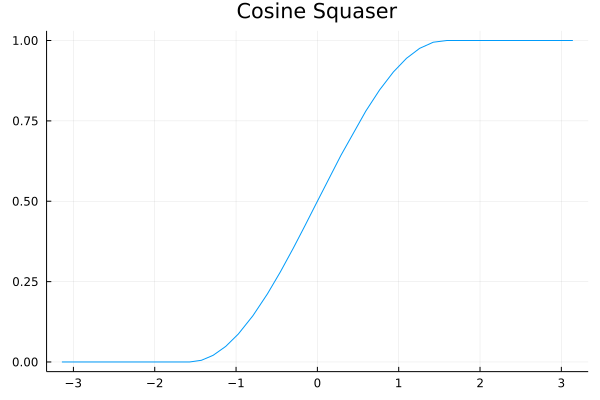
\includegraphics[width=.7\textwidth]{articulo_rrnn_aproximadores_universales/cosineSquaser.png}
        \caption{Función \textit{cosine squaser}}
        \label{fig:cosine_squaser}
    \end{figure}

    Se tiene pues que para cualquier $\lambda \in \left[ \frac{-\pi}{2}, \frac{\pi}{2}\right]$

    \begin{equation}
        2 F(\lambda)-1 = \cos \left( \lambda - \frac{\pi}{2}\right)
    \end{equation}

    Que haciendo $\mu = \lambda - \frac{\pi}{2}$ resulta que para cualquier
    $\mu \in [-\pi, 0]$
    \begin{equation}
        \cos(\mu) = 2 F \left(\mu + \frac{\pi}{2} \right)  -1 
    \end{equation}

    Además, puesto que $F(\mu + 2 \pi M) = 1$ para todo $\mu \in [-M, M] \supset [-\pi, 0]$ tenemos que
    para cualquier $\mu \in [-\pi, 0]$
    \begin{equation}
        \cos(\mu) = 2 F \left(\mu + \frac{\pi}{2} \right)  - F(\mu + 2 \pi M) 
    \end{equation}

    \begin{figure}[h]
        \centering
        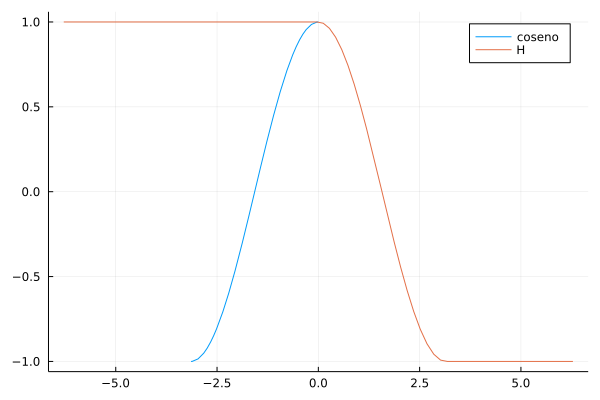
\includegraphics[width=.7\textwidth]{articulo_rrnn_aproximadores_universales/H_menos_pi_0.png}
        \caption{Comparativa $H_{[-\pi, 0]}$ con la función coseno real. }
        \label{fig:coseno_vs_H_menos_pi_cero}
    \end{figure}

    De manera generalizada denotaremos como $H_{[M_1,M_2 ]}$ a la función 
     existe $H_{[M_1,M_2 ]} \in \sum(F)$ 
    tal que para todo elemento $\lambda \in [M_1, M_2]$ se cumpla que 
    \begin{equation}
        H_{[M_1,M_2 ]}(\lambda) = \cos(\lambda)
    \end{equation}

    Por tanto $H_{[-\pi, 0]}$ viene definida como  
    \begin{equation}
        H_{[-\pi, 0]} = 2 F \left(\mu + \frac{\pi}{2} \right)  - F(\mu + 2 \pi M) 
    \end{equation}

    Por la simetría de la función coseno resulta que 
    para todo $\mu \in [0, \pi]$
    \begin{equation}
        \cos(\mu) = \cos(-\mu) = H_{[-\pi, 0]}(-\mu)
    \end{equation}
    \begin{figure}[h]
        \centering
        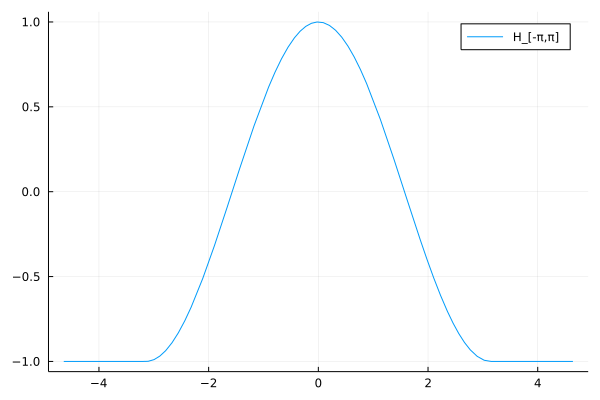
\includegraphics[width=.7\textwidth]{articulo_rrnn_aproximadores_universales/H_menos_pi_mas_pi.png}
        \caption{Función $H_{[-\pi, \pi]}$. }
        \label{fig:H_menos_pi_mas_pi}
    \end{figure}

    Así pues podemos definir 
    \begin{equation}
        \begin{split}
            H_{[-\pi, \pi ]}(\mu) &= H_{[-\pi, 0]}(\mu) + H_{[-\pi, 0]}(-\mu) - 1 \\
            &= H_{[-\pi, 0]}(\mu) + H_{[-\pi, 0]}(-\mu) - F(\mu + 2 \pi M). 
        \end{split} 
    \end{equation}  

    Por ser el coseno una función periódica es fácil ver que 
    considerando un natural $N$ que satisfaga que $2 \pi N \geq M$
  
    \begin{equation}
    \begin{split}
        H_{[-2\pi N, 2 \pi N]} (\lambda) = 
        \sum_{i=1}^N (H_{[-\pi, \pi ]}(\lambda + 2 \pi i) +1) 
        + H_{[-\pi, \pi ]}(\lambda)  \\
        - \sum_{i=1}^N (H_{[-\pi, \pi ]}(- \lambda + 2 \pi i - \pi) +1),
    \end{split}
\end{equation}
\begin{equation}
    \begin{split}
        H_{[-2\pi N, 2 \pi N]} (\lambda) 
        =  H_{[-\pi, \pi ]}(\lambda) + 
        \sum_{i=1}^N (
            H_{[-\pi, \pi ]}(\lambda + 2 \pi i)
            - 
            H_{[-\pi, \pi ]}(- \lambda + 2 \pi i - \pi)
        ) .         
    \end{split}
    \end{equation}

      % Ejemplos de la función H final
      \begin{figure}[h]
        \centering
        \begin{subfigure}[b]{0.45\textwidth}
            \centering
            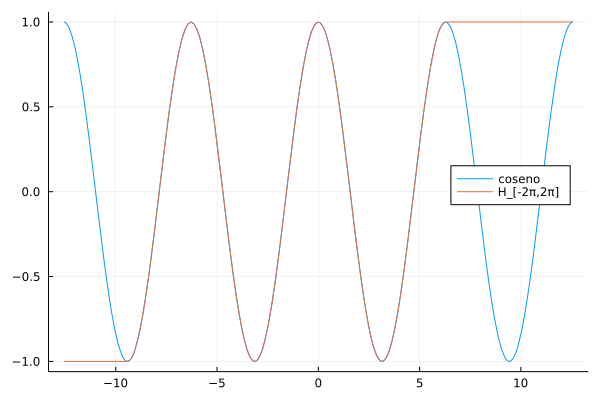
\includegraphics[width=\textwidth]{articulo_rrnn_aproximadores_universales/H_[-2π,2π].png}
            \caption{Función $H_{[-2\pi, 2\pi]}$ con $N=1$.}
            \label{fig:H_con_M}
        \end{subfigure}
        \hfill
        \begin{subfigure}[b]{0.45\textwidth}
            \centering
            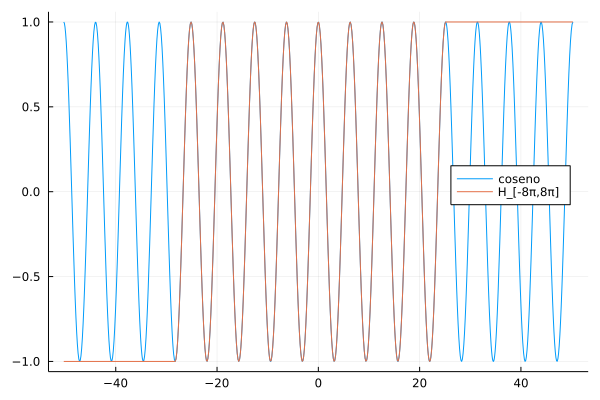
\includegraphics[width=\textwidth]{articulo_rrnn_aproximadores_universales/H_[-8π,8π].png}
            \caption{Función $H_{[-8\pi, 8\pi]}$ con $N=4$. }
        \end{subfigure}
        \hfill
        \caption{Ejemplos de funciones $H_{[-M, M]}$}
    \end{figure}

    Está claro que por ser $2 \pi N \geq M$ la función $H_{[-M, M]}$ será la restricción de la anterior, es decir: 

    \begin{equation}
        H_{[-M, M]} = H_{[-2\pi N, 2 \pi N]_{|[-M, M]}}.
    \end{equation}

    
    Así definida $H_{[-2\pi N, 2 \pi N]}$
    pertenecerá a $\sum(F)$ o lo que es de nuestro interés, estará 
    formada por una combinación finita, supongamos que $K$, 
    sumas y restas finita de $F \circ A_i$ con $A_i$ una función afín. 
    Por ser $F$ una función de activación continua gracias al
    lema \ref{lema:a_2_paso_previo_denso}, 
    existirá $W_{ \frac{\epsilon}{k}} \in \sum(\psi)$ tal que 
    podremos acotar $|F - W_{ \frac{\epsilon}{k}} | < \frac{\epsilon}{k}$ en todo $\R$.

    Además, como las transformaciones afines $A_i$ solo son traslaciones,
    para cada $i \in \{1,..K\}$ se cumple que 
     $W_{ \frac{\epsilon}{k}} \circ A_i \in \sum(\psi)$ y se mantiene que 
    \begin{equation}
        |F \circ A_i - W_{ \frac{\epsilon}{k}} \circ A_i | < \frac{\epsilon}{k}. 
    \end{equation}


    Recopilemos pues, tenemos que para $2\pi N \geq M$ y en el dominio $\lambda \in [-M, M]$: 
    \begin{equation}
        H_{[-M, M]} (\lambda) = 
        H_{[-2\pi N, 2 \pi N]}(\lambda) = 
        \sum_{i=1}^k \alpha_i F( A_i(\lambda)) \quad \alpha_i \in \{-1,1\}.
    \end{equation}
    fijando tales $\alpha_i \in \{-1,1\}$ y las traslaciones $A_i$ definimos 
    \begin{equation}
        \cos_{M, \epsilon}(\lambda) = \sum_{i=1}^k 
        \alpha_i  W_{ \frac{\epsilon}{k}}(A_i(\lambda)). 
    \end{equation}

    De esta manera, para cualquier $\lambda \in [-M, M]$

    \begin{equation}
        \begin{split}
            |\cos_{M,\epsilon}(\lambda) - \cos(\lambda)| 
            &= |\cos_{M,\epsilon}(\lambda) - \cos(\lambda) \pm  H_{[- M, M]}(\lambda)| \\
            &\leq
            |\cos(\lambda) -  H_{[- M, M]}(\lambda)|
            + 
            | \cos_{M,\epsilon}(\lambda) -  H_{[- M, M]}(\lambda)|  \\
            &\leq  0 
            + | \cos_{M,\epsilon}(\lambda) -  H_{[- M, M]}(\lambda)| \\
            & \leq  \sum_{i=1}^k 
            |  W_{ \frac{\epsilon}{k}}(A_i(\lambda)) 
            -
            F( A_i(\lambda))
             | \\
             & <   \sum_{i=1}^k \frac{\epsilon}{k} = \epsilon .
        \end{split}
    \end{equation}

    Dando con esto por concluida la demostración. 
 
\end{proof}

%Lema 4.A
\begin{lema}
    Sea $g(\cdot) = \sum_{j=1}^q \beta_j \cos(A_j(\cdot))$ con 
    $A_j \in A^r$. 
    Para cualquier función de activación $\psi$, 
    cualquier compacto $K \subset \R^r$
    y cualquier $\epsilon > 0$
    existe $f \in \sum^r(\psi)$ para el cual se cumple que 
    \begin{equation}
        \sup_{x \in K} 
        |g(x) - f(x)| < \epsilon.
    \end{equation}
\end{lema}

%Lema A.5 
\begin{lema}
    Para cualquier función de activación $\psi$ se tiene que 
    $\rrnn$ es uniformemente denso en compactos de $C^r.$
\end{lema}

% Teorema 2.4
\begin{teorema}
    Para cualquier función de activación $\psi$, $r \in \N$ y
    medida de probabilidad $\mu$ o $(\R^r, B^r)$, 
    se tiene que $\rrnn$ es uniformemente denso en compactos
    en $\fC$ y denso en $\fM$ de acorde a la distancia $\dist$. 
\end{teorema}
% !TeX root = ../../tfg.tex
% !TeX encoding = utf8
%
%***************************************************************
% Contenido del artículo 4: Colorario 2.1
%***************************************************************

% Resultado de teoría de la medida 
Trataremos ahora de generalizar la tesis expuesta en 
 el teorema \ref{teo:2_4_rrnn_densas_M} sobre las funciones medibles. 
 Para ello recordaremos el teorema de Lusin.
% Teorema de Lusin 
\begin{teorema}[Teorema de Lusin] \label{teo:Lusin}
    Si $\mu$ es una medida regular de Borel, $E$ un conjunto de medida finita 
    y $f$ una función medible en $E$ entonces
    para cualquier $\epsilon > 0$ existirá un conjunto compacto 
    $K$ en $E$ tal que $\mu(E \setminus C) \leq \epsilon$ y donde $f$ es continua en $K$. 
\end{teorema}
\begin{proof}
    Demostración en páginas 242 y 243 de \cite{nla.cat-vn1819421}.
\end{proof}  

Notemos los puntos clave de este teorema, nos va a permitir \textit{trabajar} con una función medible como si fuera continua en un compacto
todo lo parecido a $\R^r$ como se quiera. 
 
\begin{teorema}(Caracterización de normalidad de Tietze)\label{teo:Tietze}
    Sea $X$ un espacio Hausdorff. Son equivalentes las siguientes afirmaciones: 
    \begin{enumerate}
        \item $X$ es normal.
        \item Para cada conjunto cerrado $A \subset X$ y para cualquier función continua 
        $f: A \longrightarrow \R$, $f$ admite una extensión continua $F:X \longrightarrow \R.$
        Además, si para todo $a \in A$ se cumple que $|f(a)| < c \in \R$, se puede elegir $F$
        de tal forma que satisfaga que $|F(x)| < c$ para todo $x\in X.$ 
    \end{enumerate}
    (Demostración en páginas 149-151 de \cite{james1966topology})
\end{teorema}

Como el ambiente actual en el que estamos trabajando 
es el espacio $(\R^r, \mathcal{T})$ que sabemos que es normal y puesto que es habitual que nuestras funciones estén definidas
en  compactos de $\R^r$, las podremos extender a $\R^r$. 


% Corolarios del artículo 
% Corolario 2.1
\begin{corolario} \label{cor:2_1}
    Para cada función $g \in \fM$ existe un subconjunto compacto 
    $K$ de $\R^r$ y $f \in \rrnn$ tal que para cualquier 
    $\epsilon > 0$ se tiene que 
    $\mu(K) > 1- \epsilon$ y para cada $x \in K$ tenemos que 
    \begin{equation}
        |f(x) - g(x) | < \epsilon,
    \end{equation}
    independientemente de la función de activación $\psi$, dimensión $r$ o medida $\mu$. 
\end{corolario}

    \marginpar{
    \textcolor{dark_green}{
        \textbf{Idea intuitiva corolario \ref{cor:2_1}}
    }
    }
    \marginpar{
    Este teorema corrige la carencia sobre la precisión del error que describíamos en la idea intuitiva del teorema \ref{teo:2_4_rrnn_densas_M}. Podemos encontrar una red neuronal que aproxime cualquier función medible que queramos en todos los puntos del espacio que queramos.
    }

    
\begin{proof}
    Sea $\epsilon > 0$ fijo pero arbitrario.  Gracias al teorema de Lusin \ref{teo:Lusin}
    existe un subconjunto compacto $K \subset \R^r$ de medida
    $\mu(K) > 1 - \epsilon$ donde la restricción  $g_{|K}$ es continua. 

    Por otra parte, en virtud de la caracterización de Tietze 
    \ref{teo:Tietze}, 
    por estar $g_{|K}$ definida en un compacto, admite una 
    extensión continua $G:\R^r \longrightarrow \R$ tal que 
    \begin{equation}
        \begin{split}
            G_{|K} = g_{|K} .
        \end{split}
    \end{equation}

    Por ser $G$ continua en un compacto, por la densidad de las redes neuronales en compactos en $\fC$(lema \ref{lema:A_5_uniformemente_denso_compactos} ) se tiene que existirá 
     $f \in \rrnng$ tal que 
    \begin{equation}
        \sup_{x \in K} |G(x) - f(x)| < \epsilon.
    \end{equation}

    Por lo que podemos afirmar que para todo $x \in K$
    \begin{equation}
        |f(x) -g(x)| 
        \leq 
        | f(x) -G(x)| + |G(x) -g(x)|
        < \epsilon + 0 = \epsilon
    \end{equation}
    como queríamos probar.
\end{proof}



% !TeX root = ../../tfg.tex
% !TeX encoding = utf8
%
%***************************************************************
% Contenido del artículo 5: Colorarios LP
%***************************************************************
\section{Generalización a espacios $L_p$}  
\label{ch04:espacios-Lp}
Hasta ahora habíamos considerado el espacio de funciones continuas 
$\fC$ 
como subespacio dentro del espacio de funciones medibles $\fM$. 
Sin embargo, ser continua es una hipótesis muy estricta ya que existe una amplia gama de subespacios que contienen al de 
las funciones continuas y están contenidos en el de funciones medibles. 
Es por ello que vamos a realizar una generalización de los teoremas
para espacios $L_p$. De manera intuitiva estos espacios nos van a 
permitir considerar funciones que no necesariamente sean continuas
y que incluso no están acotadas. 

 % Nota intuitiva sobre la definición  LP
 \normalmarginpar
 \marginpar{\maginLetterSize\raggedright
 \iconoAclaraciones \textcolor{dark_green}{ 
     \textbf{Idea intuitiva de espacio $L_p$}
 }
 }
 \marginpar{\maginLetterSize
 Con esta definición lo que se trata es de considerar funciones 
 que tomen un valor real en la mayoría de sus puntos.
 Ya que la integral no varía su valor si se aplican cambios puntuales. 
 }
\begin{definicion}[Espacios Lp]
    Se llama espacio $L_p(\R^d, \mu)$ o simplemente $L_p$ al conjunto 
    de funciones $f \in \fM$ tales que 
    \begin{equation}
        \int |f(x)|^p d\mu < \infty. 
    \end{equation}  
Se define la norma de $L_p$ como 
\begin{equation}
    \| f\|_p 
    =
    \left(\int |f(x)|^p d\mu \right)^\frac{1}{p}
\end{equation}
y la distancia asociada al espacio $L_p$ se define como 
\begin{equation}
    \rho_p(f,g) = \| f-g\|_p.
\end{equation}
\end{definicion}


% Corolario 2.2
\begin{corolario}\label{corolario:2_2_rrnn}
    Si existe un subconjunto compacto $K$ en $\R^d$ de medida
    $\mu(K) =1$ entonces $\rrnn$ es $\dlp$-denso en $L_p(\R^d, \mu)$
    para cualquier $p \in [1,\infty)$, independientemente de 
    $\psi$, $d$ o $\mu$.
\end{corolario}

% Nota intuitiva sobre el corolario 2.2
\marginpar{\maginLetterSize\raggedright
    \iconoAclaraciones \textcolor{dark_green}{ 
        \textbf{Idea intuitiva corolario \ref{corolario:2_2_rrnn}}
    }
}
\marginpar{\maginLetterSize
Se prueba que las redes neuronales son capaces de aproximar 
cualquier función de la clase recién introducida.
}


\begin{proof}
    Se quiere probar que para cualquier $g \in L_p$ y 
    $\varepsilon >0$ existe $f \in \rrnn$ tal que 
    \begin{equation}
        \dlp(f,g) <\varepsilon.
    \end{equation}   
    
    Por pertenecer $g$ a $L_p$ existe una constante $M$ real positiva
    lo suficientemente grande 
    tal que si definimos la función $h =g 1_{|g|<M}$ esta satisface 
    que
    \begin{equation}\label{eq:corolario_2_2:h_compacto}
        \dlp(g,h) < \frac{\varepsilon}{3}.
    \end{equation}
    
    Además como $h$ es una función acotada de $L_p$, podemos encontrar
    una función $s$ continua que es límite de una sucesión de
    funciones simples 
    ( pag 241-242,  teoremas 55C y 55D \cite{nla.cat-vn1819421})
    y la cual cumple que 

    \begin{equation}\label{eq:corolario_2_2:s_continua}
        \dlp(h,s) < \frac{\varepsilon}{3}.
    \end{equation}

    Por el teorema \ref{teo:2_4_rrnn_densas_M}, al estar en un compacto $K$ y por ser $\rrnn$ uniformemente
    denso en compactos hay una $f \in \rrnn$ la cual cumple que
    \begin{equation}
        \sup_{x \in K} |f(x) -s(x)|^p 
        <
         \left( \frac{\varepsilon}{3}\right) ^p.
    \end{equation}
    
    Y por hipótesis $\mu(K) =1$ y definición de la distancia $\dlp$ 
    se tiene la siguiente desigualdad: 

    \begin{equation} \label{eq:corolario_2_2:cota_rrnn}
        \dlp(f,s) = 
        \left(\int |f(x) - s(x)|^p d\mu \right)^\frac{1}{p}
        \leq 
        \left(\int  \left( \frac{\varepsilon}{3}\right) ^p d\mu \right)^\frac{1}{p}
        = \left( \mu(K)  \left(\frac{\varepsilon}{3} \right)^p\right) ^\frac{1}{p}
        = \frac{\varepsilon}{3}.
    \end{equation}

    Gracias a la desigualdad triangular y las desigualdades
    (\refeq{eq:corolario_2_2:cota_rrnn}),
    (\refeq{eq:corolario_2_2:h_compacto}) y 
    (\refeq{eq:corolario_2_2:s_continua})
    tenemos
    \begin{equation}
        \dlp(f,g) 
        \leq
            \dlp(f,s)
            +\dlp(s,h)
            + \dlp(h,g)
        < 
        \frac{\varepsilon}{3} + \frac{\varepsilon}{3} + \frac{\varepsilon}{3}
        = \varepsilon.
    \end{equation}
Probando con ello lo buscado. 
\end{proof}  

% Corolario 2.3
\begin{corolario}\label{corolario:2_3_medida_probabilidad}
    Si $\mu$ es una medida de probabilidad en $[0,1]^d$
    entonces 
    $\rrnn$ es $\dlp$-denso en 
    $L_p([0,1]^d, \mu)$ para todo $p \in [1, \infty)$,
    independientemente de $\psi, d, \mu$. 
\end{corolario}

% Nota intuitiva sobre el corolario 2.3
\marginpar{\maginLetterSize\raggedright
    \iconoAclaraciones \textcolor{dark_green}{ 
        \textbf{Idea intuitiva corolario 
        \ref{corolario:2_3_medida_probabilidad}}
    }
}
\marginpar{\maginLetterSize
    A diferencia que con el corolario \ref{corolario:2_2_rrnn},
aquí se afirma que las redes neuronales son capaces de aproximar 
cualquier función de la clase recién introducida cuyo dominio parta de $[0,1]^d$, es decir \textbf{se está concretando los valores de entrada que pueden tomar las funciones}.
}


\begin{proof}
    Es consecuencia directa del corolario previo \ref{corolario:2_2_rrnn}
    donde para este caso particular $K = [0,1]^d$ un compacto
    de $\R^d$
    que cumple que $\mu(K) = 1.$
\end{proof}

%Corolario 2.4 
\begin{corolario} \label{corolario:2_4_conjunto_finito}
    Sea $\mu$ una medida, que para
    un conjunto finito de puntos $O$ cumple que $\mu(O)=1$, 
    entonces, para cualquier función medible $g \in \fM$
    y sea cual sea $\varepsilon >0$ 
    existe $f \in \rrnn$ la cual cumple que 
    \begin{equation}
        \mu\{ 
            x:
            |f(x) - g(x)| 
            < \varepsilon
        \}
        = 1.
    \end{equation}

\end{corolario}
\begin{proof}
    Por el teorema \ref{teo:2_4_rrnn_densas_M} existe 
    $f \in \rrnn$ tal que para cualquier 
    $\varepsilon_1, \varepsilon_2 >0$ se cumple que 
    $\mu \{x: |f(x) - g(x)| > \varepsilon_1\} < \varepsilon_2.$
    Sea $O$ el conjunto de puntos tal que $\mu(O) = 1.$
    Por ser finito $O$ podemos encontrar
    \begin{equation} \label{eq:2_4:definición_epsilon}
        \delta = \min_{x \in O} \{ 
            \mu(x) : \mu(x)>0
        \}. 
    \end{equation}

    Sin pérdida de generalidad tomamos $\varepsilon < \delta$ y entonces
    para  que la $f$ fijada cumpla que
    \begin{equation}
        \dist(f,g) = \varepsilon
    \end{equation}
    debe de cumplirse que 
    \begin{equation}
        \dist(f,g) =  \inf 
        \{
           \varepsilon_1 > 0:
           \mu\{ 
            x:
            |f(x) - g(x)| 
            > \varepsilon_1
        \}
        < \varepsilon_1
        \} 
        = \varepsilon,
    \end{equation}
    pero por cómo tomamos $\varepsilon$ en (\refeq{eq:2_4:definición_epsilon}) se
    tiene que $\mu\{ 
        x:
        |f(x) - g(x)| 
        > \varepsilon
    \} = 0.$
    Por lo que acabamos de probar, como queríamos, que 
    \begin{equation}
        \mu\{ 
            x:
            |f(x) - g(x)| 
            < \varepsilon
        \}
        = 1.
    \end{equation}
\end{proof}

Nótese que con este corolario lo que se está indicando es que dado
un conjunto finito y sus respectivas imágenes, se puede encontrar una red neuronal que para tales puntos \textit{devuelva} el valor exacto. 
%Nota aclarativa sobre la relevancia del corolario
\marginpar{\maginLetterSize
    \iconoAclaraciones \textcolor{dark_green}{     
        \textbf{
            Relevancia práctica del corolario 
            \ref{corolario:2_5_función_Booleana}
        }
    }
     
    Este resultado nos permite \textbf{aproximar funciones que actúen como clasificadores discretos}. Por ejemplo sea $g$ como una función que dada una imagen $x$ indica si hay un perro haciendo valer $g(x)=1$ y en caso contrario $g(x)=0$.
      
}

%Nota aclarativa sobre la implementación del corolario
\marginpar{\maginLetterSize
    \textcolor{red}{    
        \textbf{
            Observación sobre la implementación
            del corolario
            \ref{corolario:2_5_función_Booleana}
        }
    }
    
    El resultado nos   indica que podemos obtener una red neuronal $h$ que aproxime tal clasificador, 
    pero \textbf{tal red neuronal no necesariamente tomará valores discretos}, es decir,
     pudiera darse el caso en que las imágenes 
     a un rango, por ejemplo: 
     $$h( \{ x : g(x)=0 \})  \subset [-0.2,0.3]$$ 
     y que 
     $$h(\{ x : g(x)=1 \})  \subset [0.9,1.2],$$ 
     por lo que se pone de manifiesto en este
      resultado, 
     que en caso de requerirse
      de una salida completamente
     discreta debería de componerse 
     con otra función $\theta$ 
     tal que 
     $$\theta \circ h(\{ x : g(x)=0 \})=0$$ y 
     $$\theta \circ h(\{ x : g(x)=1 \})=1$$.
    
}

\begin{definicion}[Función Booleana]
    Decimos que una función es Booleana si su dominio es 
    $\{0,1\}^d$  para algún $d \in \N \setminus \{0\}$
    y su codominio es $\{0,1\}$. Es decir,
    \begin{equation}
      f:\{0,1\}^d \longrightarrow \{0,1\}.
    \end{equation}
\end{definicion}

Ejemplos conocidos son la función 
$or: \{0,1\}^d \longrightarrow \{0,1\}$  que vale 
uno si alguno de su entrada es uno y la función 
$and: \{0,1\}^d \longrightarrow \{0,1\}$
que se define como $and(x_1, \ldots, x_d) = \prod_{i=1}^d x_i.$

% Corolario 2.5  
\begin{corolario}\label{corolario:2_5_función_Booleana} 
    Para cada función Booleana 
    $g: \{0,1\}^d \longrightarrow \{0,1\}$
     y 
    cada $\varepsilon >0$ existe una red neuronal
    $f \in \rrnn$ tal que 
    \begin{equation}
        \max_{x \in \{ 0,1\}^d} |g(x) - f(x)|
        < \varepsilon.
    \end{equation}
\end{corolario}



\begin{proof}
    Se define la función $\mu : \R^d \longrightarrow [0,1]$ de forma que 
    \begin{equation}
        \mu(x) = 
      \left \{
    \begin{aligned}
      \frac{1}{2^d} \quad &\text{ si } x \in \{0,1\}^d \\
      0 \quad & \text{ si } x \notin \{0,1\}^d 
    \end{aligned}
  \right .
    \end{equation}

    Se tiene que $\mu$ es una medida ya que cumple que 
    \begin{enumerate}
        \item Hipótesis de acotación: $0 \leq \mu(A) \leq 1$ para $A \in \mathcal{P}(\R^d).$
        \item La probabilidad del vacío es nula y la del  total es la unidad. 
        \item La probabilidad de la unión es la suma de la probabilidades. 
        \begin{equation}
            P\left(
                \cup_{i=1}^n A_i
            \right)
            = \sum_{i=1}^n P(A_i).
            \quad
            \forall A_i \in  \mathcal{P}(\R^d).
        \end{equation}
    \end{enumerate}  

    Como la cardinalidad de $\{0,1\}^d$ es $2^d$
    podemos aplicar el corolario \ref{corolario:2_4_conjunto_finito}
    y entonces sabemos que  existe $f\in \rrnn$ tal que 
    \begin{equation}
            \mu\{ 
                x:
                |f(x) - g(x)| 
                < \varepsilon
            \}
            = 1,
    \end{equation} 
    es decir que 
    \begin{equation}
        \max_{x \in \{ 0,1\}^d} |g(x) - f(x)|
        < \varepsilon
    \end{equation}
    como queríamos probar. 
\end{proof}


% Lemas propios  previos al teorema 2.5
\begin{lema} \label{lema:propio_1_antes_teorema_2_5}
    Si una función de activación  $\psi$ alcanza el cero y el uno, esto es 
    si existen dos constantes reales $M_1, M_2$ 
    tales que 
    \begin{equation}
        \psi(M_1) = 0 \text{ y } \psi(M_2)=1
    \end{equation}
    entonces existe una constante real positiva $M$ tal que 
    \begin{equation}
        \psi(-M) = 1- \psi(M) = 0.
    \end{equation}
\end{lema}
\begin{proof}
Sea $M = \max \{|M_1|,|M_2|\}$ y por ser $\psi$ una función de activación sabemos que
es no decreciente y que su imagen pertenece al intervalo $[0,1].$

Por tanto
\begin{align}
      0 &\leq \psi(-M) \leq \psi(M_1) = 0 \quad \text{ luego } \quad \psi(-M) = 0, \\
      1 &\geq \psi(M) \geq \psi(M_2) = 1 \quad \text{ luego } \quad\psi(M) = 1.
\end{align}

Gracias a estas desigualdades es fácil ver que 
\begin{equation}
    \psi(-M) = 1 - \psi(M) = 0
\end{equation}
como queríamos probar. 
\end{proof}   

Es interesante percatarse de que de no exigirse la hipótesis de 
que $\psi$ alcanza el cero y el uno no puede 
asegurarse la igualdad demostrada. Pongamos como ejemplo la siguiente función de activación

\begin{equation}
    \psi(x)= \left\{ \begin{array}{lcc}
        0 &   si  & x \leq 0 \\
        \frac{| x |}{1+ | x |}&  si & 0< x. 
        \end{array}
    \right. 
\end{equation}


% Otro lema propio antes de probar el teorema 2.5
\begin{lema}\label{lema:previo_propio_2_al_teorema_2_5}
    Dado un conjunto finito de vectores $\Lambda \subset \R^d$ con 
    $d$ natural positivo. 
    Existe un vector $p \in \R^d$ que satisface que 
    para cualesquiera $x,y \in \Lambda$ diferentes 
    \begin{equation}
        p \cdot(x-y) \neq 0.
    \end{equation}
\end{lema}
% Nota intuitiva sobre el Teorema 2.5
\marginpar{\maginLetterSize\raggedright
    \iconoAclaraciones \textcolor{dark_green}{ 
        \textbf{Idea clave teorema
        \ref{teorema:2_5_entrenamiento_redes_neuronales}}
    }
}
\marginpar{\maginLetterSize
   Podemos conseguir una red neuronal que \textit{valga} lo que queramos en un conjunto finito de puntos.
}
% Prueba lema propio antes de probar el teorema 2.5
\begin{proof}
    Si $n$ es el cardinal de $\Lambda$,
    consideramos el conjunto $U$ definido como la unión de 
    $n (n-1)$ hiperplanos de $\R^d$

    \begin{equation}
        U = \bigcup_{ 
            \substack{
                x,y \in \Lambda \\
                x \neq y
            }
        }
        \{ 
            p \in \R^d: p \cdot (x-y) = 0
        \}.
    \end{equation}

    Puesto que $\R^d$ no puede ser expresado como unión finita de hiperplanos,
    $U \subsetneq \R^d$ y por tanto existirá $p \in \R^d \setminus U$ tal que 
    \begin{equation}
        p \cdot(x-y) \neq 0 
        \text{ para cualesquiera }
         x,y \in \Lambda \text{ diferentes, }
    \end{equation}
    como queríamos probar. 
\end{proof}

% Nota intuitiva sobre la demostración del Teorema 2.5
\setlength{\marginparwidth}{\smallMarginSize}
\marginpar{\maginLetterSize\raggedright
    \iconoAclaraciones \textcolor{dark_green}{ 
        \textbf{Idea de la demostración del teorema
        \ref{teorema:2_5_entrenamiento_redes_neuronales}}
    }
}
\marginpar{\maginLetterSize
    {
  Es interesante reparar en que la demostración se basa
  en añadir una neurona por cada punto que queramos que tome
  un valor concreto, esa neurona se activará (es decir, no será nula) cuando la entrada $x$ \textit{sea mayor} que el valor que la activa $x_i$ y vale la diferencia con el valor anterior $x_{i-1}$, es decir $g(x_{i}) - g(x_{i-1})$, como el nodo $x_{i-1}$
  también se activará por ser menor, el término $g(x_{i-1})$ se suma a la salida de la red y así como una serie telescópica al final solo resultará el valor $g(x_i)$.
    }
}
\setlength{\marginparwidth}{\bigMarginSize}
% fin de la nota


% Teorema 2.5  
\begin{teorema}[Sobre el entrenamiento práctico de redes neuronales]
    \label{teorema:2_5_entrenamiento_redes_neuronales}
    Sea $ \Lambda = \{x_1, \ldots, x_n\}$ un conjunto de puntos distintos de 
    $\R^d$ y sea 
    $g: \R^d \longrightarrow \R$ una función arbitraria. 
    Si $\psi$ alcanza el cero y el uno, 
    entonces
    existe una red neuronal $f \in \rrnn$ con $n$
    neuronas ocultas tal que 
    \begin{equation}
        f(x_i) = g(x_i) \text{ para todo } i \in \{1, \ldots, n \}.
    \end{equation}
\end{teorema}

\begin{proof}
Con el fin de facilitar la comprensión dividiremos la demostración en dos casos, 
primero uno particular, cuando $d=1$ y después el caso general.

\textbf{Caso primero}

Suponemos que $\{x_1, \ldots, x_n\} \subset \R$ y tras renombrar 
podemos suponer que 
\begin{equation}
    x_1 < x_2 < \cdots < x_n. 
\end{equation}

Por alcanzar la función de activación $\psi$ el cero y el uno, 
gracias al lema  \ref{lema:propio_1_antes_teorema_2_5} existe una constante $M$ tal que $\psi(-M) = 1-\psi(M) = 0.$

Definiremos de manera recursiva la red neuronal buscada $f_n$.

% Nota nueva hipótesis de optimización del Teorema 2.5

\marginpar{\maginLetterSize\raggedright
     \iconoProfundizar \textcolor{blue}{
        \textbf{Nueva hipótesis de optimización}
    }
}
\marginpar{\maginLetterSize
    \textbf{
    El teorema 
        \ref{teorema:2_5_entrenamiento_redes_neuronales}
        nos brinda una heurística de inicialización de los pesos
        de una red neuronal.
    }
    La cual se tratará en la sección \ref{section:inicializar_pesos}.
\setlength{\marginparwidth}{\bigMarginSize}
 
}

\begin{itemize}
    \item Red neuronal $f_1$. 

Sea $A_1$ la función afín constante $A_1 = M.$
Fijamos $\beta_1 = g(x_1)$. 
De esta manera la red neuronal $f_1$ queda
definida como $f_1(x) = \beta_1 \psi(A_1(x)).$

\item Red neuronal $f_k$ con $1 < k \leq n$. 

Se define $A_{k}$ como la única función afín que cumple que 
\begin{equation}
    A_k(x_{k-1}) = -M \quad \text{y} \quad  A_{k}(x_k)= M.
\end{equation}
Fijamos $\beta_k = g(x_k) - g(x_{k-1})$. 
La red neuronal $f_k$ se calcula como 
\begin{equation}
    f_k(x) 
    = 
    \sum_{j=1}^k \beta_j \psi(A_j(x))
     = 
    (g(x_k)-g(x_{k-1})) \psi(A_k(x)) + f_{k-1}(x) .  
\end{equation}
Observemos que así construida se tiene que para cualquier
 $y > x_k$ la evaluación con la red neuronal resulta $f_k(y) = g(x_k).$
\end{itemize}

Veamos por inducción sobre $n$ que así definida para cualquier $1 \leq i \leq n$ se tiene que     
$f_n(x_i) = g(x_i)$. 
Además de que tiene un total de $n$ neuronas ocultas. 


\begin{itemize}
    \item Caso base, $n=1$. 
    \begin{equation}
        f_1(x_1)= \beta_1 \psi(A_1(x_1)) = g(x_1)\psi(M) = g(x_1).
    \end{equation}
    \item Supuesto que es cierto para $n-1$ veamos que lo es para $n$.      
    Evaluación de $x_n$
    \begin{align}
        f_n(x_n) 
        &= 
        (g(x_n) - g(x_{n-1}))\psi(A_n(x_n)) + f_{n-1}(x_n)
        \\
        & = (g(x_n) - g(x_{n-1}))\psi(M) + g(x_{n-1}) 
        \\
        & = (g(x_n) - g(x_{n-1})) + g(x_{n-1}) 
        \\
        & = g(x_n).
    \end{align}

Evaluación de $x_i$ con $1 \leq i < n$. 

Usando que $0 \leq \psi(A_n(x_i)) < \psi(A_n(-M)) = 0$ y la hipótesis de inducción se tiene que 
\begin{align}
    f_n(x_i) 
        &= 
        (g(x_n) - g(x_{n-1}))\psi(A_n(x_i)) + f_{n-1}(x_i)
        \\
        & = 0 + g(x_{i}) 
        \\
        &= g(x_i).
\end{align}
\end{itemize}

Acabamos de probar por inducción  que
$f_n(x) = g(x)$ para cualquier $x \in \Lambda$, lo que termina la demostración.

\textbf{Caso segundo}  

Se tiene para este caso que $\Lambda \subset \R^d$ con $d >1$. 
Seleccionamos $p \in \R^d$ cumpliendo que 
para cualesquiera $x,y \in \Lambda$ distintos 
$p(x-y) \neq 0$ (es posible de 
encontrar por el lema \ref{lema:previo_propio_2_al_teorema_2_5}).
Gracias a esta condición cada producto $p \cdot x$ con $x \in \Lambda$ es distinto y podemos establecer con ello una relación de orden, que tras 
renombrar los elementos de $\Lambda$ queda
\begin{equation}
    p \cdot x_1 < p \cdot x_2 < \cdots < p \cdot x_n,
\end{equation}
y como procedimos en el caso primero, definimos de manera
 recursiva la red neuronal $f_n$ buscada:

 \begin{itemize}
 \item Red neuronal $f_1$. 

Sea $B_1$ 
la función afín de $\R$ a $\R$ constante $B_1 = M.$
Fijamos $\beta_1 = g(x_1)$. 
De esta manera la red neuronal $f_1$ 
definida como $f_1(x) = \beta_1 \psi(B_1(p \cdot x)).$

\item Red neuronal $f_k$ con $1 < k \leq n$. 

Se define $B_{k}$ como la única función afín de $\R$ en $\R$ que cumple que 
\begin{equation}
    B_k(p \cdot x_{k-1}) = -M 
    \quad \text{y} \quad 
     B_{k}(p \cdot x_k)= M.
\end{equation}
Podemos definir entonces $A \in \afines$ por 
$A_k(x)=B_k(p \cdot x).$
Fijamos  también
$$\beta_k = g(x_k) - g(x_{k-1}).$$ 
La red neuronal $f_k$ se calcula como 
\begin{align}
    f_k(x) 
    = &
    \sum_{j=1}^k \beta_j \psi(B_j(p \cdot x))
     = 
    (g(x_k)-g(x_{k-1})) \psi(B_k(p \cdot x)) + f_{k-1}(x) \\
    \\
    & = 
    \sum_{j=1}^k \beta_j \psi(A_j(x))
    = 
   (g(x_k)-g(x_{k-1})) \psi(A_k(x)) + f_{k-1}(x).  
\end{align}
\end{itemize}

Así definida, la prueba por inducción es idéntica a la del caso primero y hemos encontrado por tanto la red neuronal $f_n$ buscada.
\end{proof}

\subsection{Reflexión sobre el número de neuronas} \label{subsection:reflexión_sobre_número_de_neuronas}

Ante la pregunta natural de 
\textit{¿cuántas neuronas son necesarias?} el 
recién probado teorema nos responde que 
si estamos entrenando con $n$ datos, con $n$ neuronas es suficiente para volver a reproducir esos datos. Pero esto carece de sentido a nivel práctico por los siguientes motivos. 

\subsubsection*{Naturaleza de los datos}  
Recordemos que el problema al que nos enfrentamos es el siguiente:
queremos ser capaces de predecir cierto fenómeno regido por $g$ una \textit{función} desconocida. 
Para ello tenemos un \textit{conjunto de muestras} 
compuestas por pares $(x, g(x))$, es decir, ante la situación $x$
hemos observado que el fenómeno se comporta como $g(x)$. Todo esta 
situación experimental puede producir incoherencias teóricas, como por ejemplo que se tengan dos muestras $(x_1, y_1), (x_2, y_2)$ 
tales que $x_1 = x_2$ pero $y_1 \neq y_2$ o que la medición contenga errores, es decir $(x, g(x)+\delta)$. 

Se podría paliar esta situación con un
 preprocesado de los datos. 

\subsubsection*{ Naturaleza de la regla subyacente}  

Supongamos que los datos de entrenamiento son perfectos. Existen infinitas aplicaciones 
que evalúan de la misma manera un conjunto finito de puntos. 
¿Cuáles tomar?

Podríamos, siguiendo el principio de economía de Ockham optar
por modelos que reduzcan el número de neuronas, pero entonces la 
pregunta sería  ¿qué número mínimo de neuronas serían necesarios para representar el modelo? 
Una solución sería tomar un número de neuronas menor que el tamaño del conjunto de 
entrenamiento y utilizar esa \textit{redundancia} de datos para 
\textit{afinar}. 

\subsubsection*{Coste computacional inasumible}  
Supongamos que los datos son idílicos, el modelo se conoce y se establece un tamaño de datos de entrenamiento suficiente y
un número de neuronas acorde  ¿podríamos asumir el coste computacional?


% !TeX root = ../../tfg.tex
% !TeX encoding = utf8
%
%***************************************************************
% Contenido del artículo 5: Generalización a multi-output 
%***************************************************************
\section{Generalización para \textit{multi-output neural networks}}
\label{ch04:salida-varias-dimensiones}
En las secciones anteriores se han provisto resultados para redes 
neuronales de salida real. Vamos a generalizar los resultados vistos
para ser capaces de aproximar funciones continuas o medibles 
de $\R^d$ a $\R^s$ con $d,s \in \N.$

Denotaremos por $\fCC$ al conjunto de funciones continuas definidas de $\R^d$ a $\R^s$ y al de funciones medibles de 
$\R^d$ a $\R^s$  por $\fMM.$ 
La distancia asociada a estos espacios se define como 
\begin{equation}
    \rho_{\mu}^s(f,g) 
    =
    \sum_{i=1}^s \dist(f_i, g_i).
\end{equation}

Con la siguiente definición buscamos abstraer el modelo de una red neuronal de una capa oculta y salida múltiple.
\begin{figure}[h]
    \centering
    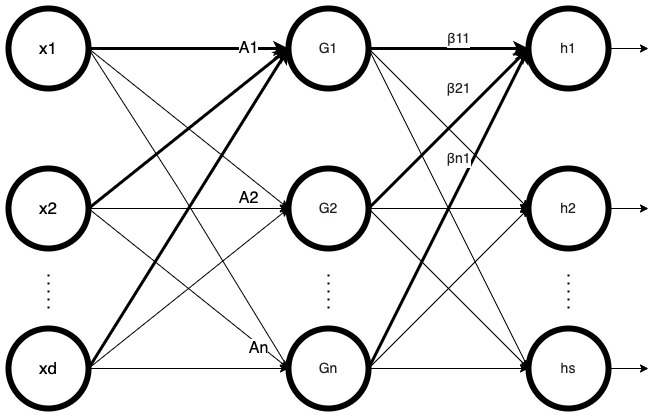
\includegraphics[width=.9\textwidth]{articulo_rrnn_aproximadores_universales/Red-Neuronal-blanco-negro-varias-salidas.jpg}
    \caption{Ejemplo de red neuronal de una capa oculta con $n$ nodos, de dimensión de entrada $d$ y salida $s$.}
    \label{fig:red neuronal-r-h-s}
\end{figure}

Nótese que los vectores $(w_{0i},w_{1 i}, \ldots, w_{r i})$ representan a la aplicación afín 
$A_i((x_1, x_2, \ldots x_r)) = w_{0i} + \sum_{j=1}^d w_{ji} x_j$
con $i \in \{1,\ldots, h\}$ . 

\begin{definicion}[Abstracción de una red neuronal con una capa oculta y múltiple salida] 
    Para cualquier función Borel medible $G$, definida de $\R$ a $\R$ y cualquiera naturales positivo
    $d,s \in \N$ se define a la clase de funciones $\rrnnmc$ como 
    \begin{equation}
        \begin{split}
        \rrnnmc = 
        \{ 
            & h: \R ^d \longrightarrow \R^s, h= (h_1, h_2, \ldots, h_s)  / \quad 
            \\ &
            \text{ con } h_i : \R ^d\longrightarrow \R, 
            h_i(x)=\sum_{j = 1} ^{n_i} (
            \beta_{j i} G(A_{j}(x)) \quad i \in \{1,2,\ldots, s\}, \\
            & x  \in \R ^d, \beta_{j i} \in \R, A_{j}\in \afines,n_i \in \N, i \in \{1,\ldots, s\} 
        \}.
        \end{split}
    \end{equation}
\end{definicion}

\iconoAclaraciones \textcolor{dark_green}{ Observación: }

% Comentario 
\marginpar{\maginLetterSize
    \iconoAclaraciones \textcolor{dark_green}{     
        \textbf{
        Por qué se ha destacado la observación
        }
    }
    Se destaca tal observación para remarcar que una 
    red neural con salidas en varias dimensiones tiene
    una definición mucho más estricta y que podría dar a confusión.
    
}

Es interesante apreciar que se tiene que 
    \begin{equation} \label{eq:diferencia_conjuntos_multicapa}
        \begin{split}
        \rrnnmc \subsetneq
        \{ 
            & h: \R ^d \longrightarrow \R^s, h= (h_1, h_2, \ldots, h_s)  / \quad 
            \\ &
            h_i \in \rrnn \quad \forall i \in \{1, \ldots, s\}
        \}.
        \end{split}
    \end{equation}
    aunque como veremos en el corolario \ref{corolario:2_6} $\rrnnmc$ es un espacio denso en el conjunto que acabamos de presentar. 
    Si tenemos presente que de acorde a nuestras definiciones una red neuronal $h_i$ viene determinada por un conjunto de funciones afines $A^{(i)}_j$  y escalares $\beta^{(i)_j}$, se daría la igualdad en \refeq{eq:diferencia_conjuntos_multicapa} si imponemos que para cualquier par de redes neuronales $h_k, h_j$ se satisface que $A^{(k)}_i = A^{(j)}_i$. 


No es difícil pensar que su versión generalizada sea: 

\begin{definicion} 
    Dadas las mismas hipótesis que en la definición anterior, se define la siguiente clase de funciones como 
    \begin{equation}
        \begin{split}
            \sum \prod^{d, s}(G) 
            = 
        \{ 
            & f: \R ^d \longrightarrow \R^s, f= (f_1, f_2, \ldots , f_s)  / \quad 
            \\ &
            \text{ con } f_i : \R ^d\longrightarrow \R, 
            f_i(x)=\sum_{j = 1} ^h 
            \left(
            \beta_{j i} \prod_{k=1}^{l_{j i}} G(A_{j i}(x))
            \right)
             \quad i \in \{1,2,\ldots, s\}, \\
            & x \in \R ^d, \beta_{j i} \in \R, A_{j i}\in \afines; h,l_{j i} \in \N 
        \}.
        \end{split}
    \end{equation}
\end{definicion}


% Corolario 2.6  
\begin{corolario}\label{corolario:2_6}
    Los teoremas 
    \ref{teorema:2_3_uniformemente_denso_compactos},
    \ref{teo:2_4_rrnn_densas_M} 
    y los corolarios
    \ref{cor:2_1}, 
    \ref{corolario:2_2_rrnn},
    \ref{corolario:2_3_medida_probabilidad},
    \ref{corolario:2_4_conjunto_finito}
    y 
    \ref{corolario:2_5_función_Booleana}
    permanecen válidos si se sustituye $\rrnn$ por $\rrnnmc$
    ,$\rrnng$ por $\rrnngmc$, 
    los espacios de funciones continuas y medibles por $\fCC$ y $\fMM$ respectivamente.
\end{corolario}

% Nota intuitiva sobre el Corolario 2.6
\marginpar{\maginLetterSize\raggedright
    \iconoAclaraciones \textcolor{dark_green}{ 
        \textbf{Idea clave corolario
        \ref{corolario:2_6}}
    }
}
\marginpar{\maginLetterSize
   En esencia, todos los resultados probados hasta ahora para redes 
   neuronales con salida real de dimensión uno son válidos para 
   cualquier tamaño de salida, es decir, \textbf{lo que a nosotros 
   nos interesa podemos aproximar cualquier función medible que 
   vaya entre espacios de dimensión finita}. 
}

% Nota intuitiva sobre la demostración del Corolario 2.6
\marginpar{\maginLetterSize\raggedright
    \iconoAclaraciones \textcolor{dark_green}{ 
        \textbf{Idea clave demostración corolario
        \ref{corolario:2_6}}
    }
}
\marginpar{\maginLetterSize
 La demostración del corolario es totalmente constructiva:
si se desea una red neuronal de salida $s\in \N$, 
se construyen de manera independiente $s$ redes neuronales de salida de dimensión uno
(una para cada salida buscada) y las concatenamos haciendo valer cero las conexiones entre nodos que no pertenecieran a las redes de partida.
}
\begin{proof}
    Observemos que todos los teoremas y lemas mencionados basan su tesis
    en la existencia de una red neuronal es decir, que si llamamos según 
    convenga $\mathcal{F}^{d,s}$ a $\rrnnmc$ o $\rrnngmc$ deberemos de 
    encontrar $f \in \mathcal{F}^{d,s}$ que cumplan las respectivas tesis para salidas múltiples. 

    La prueba se construirá por inducción sobre el número de salidas $s$. 

    % Nota nueva hipótesis de optimización del Corolario 2.6
\reversemarginpar
\setlength{\marginparwidth}{\smallMarginSize}

\marginpar{\maginLetterSize\raggedright
     \iconoProfundizar \textcolor{blue}{
        \textbf{Nueva hipótesis de optimización}
    }
}
\marginpar{\maginLetterSize
   
    La demostración del corolario nos da una \textbf{técnica constructiva}
    de obtener redes neuronales de varias salidas,
     que puede ser de valía para aplicarla \textbf{como heurística 
     para inicializar los pesos de la red neuronal} como 
     ya apuntábamos en las notas del 
   teorema 
        \ref{teorema:2_5_entrenamiento_redes_neuronales}.
}
\normalmarginpar
\setlength{\marginparwidth}{\bigMarginSize}

    El caso base $s=1$ viene dado por los respectivos teoremas y lemas ya probados.
    Supuesto cierto para $s = n$ veamos que se cumple para $s=n+1$: 
    
    Se quiere encontrar 
    $f = (f_1, f_2, \ldots, f_n, f_{n+1})$ de $n+1$ salidas, 
    por hipótesis de inducción existe $g_n \in \mathcal{F}^{d,n}$ con
     $g_n = (f_1, f_2, \ldots, f_n)$ y con $h_n$ sumandos. Denotamos a los pesos de las transformaciones afines 
     $w_{i j} \in \R$ con 
     $i \in \{0, 1, \ldots , d \}$  y  $j \in \{1, \ldots ,h_n \}$ 
     y $\beta_{ k l} \in \R$ con 
     $k \in \{1, \ldots ,h_n \}$  y  $l \in \{1, \ldots ,n \}.$

    También existe $g_1 \in \mathcal{F}^{d,1}$ cumpliendo que
    $g_1 = f_{n+1}$ con $h_1$ sumandos en la capa oculta
    y pesos  
    ${w'}_{i j} \in \R$ con 
     $i \in \{0, 1, \ldots , d \}$  y  $j \in \{1, \ldots , h_1 \}$ 
     y ${\beta '}_{ k l} \in \R$ con 
     $k \in \{1, \ldots , h_1 \}$  y  $l = {n+1}$
     (Ver figura \ref{fig:red neuronal-r-h-s} para orientarse en la notación tomada).
     
    Considerando $f$ compuesta por $h_n + h_1$ sumandos y donde sus pesos son los siguientes:

    El peso $\tilde{w}$ de las funciones afines: 
    Para cuales quiera 
    $i \in \{0, 1, \ldots  , d \}$  y  
    $j \in \{1, \ldots , h_n, h_{n} + 1, \ldots, h_n + h_1\}$  determinaremos la siguiente casuística
    \begin{enumerate}
        \item Si $1 \leq j \leq h_n$ entonces $\tilde{w}_{i j} = w_{i j}.$
        \item Si $h_n < j \leq h_n + h_1$ entonces $\tilde{w}_{i j} = w_{i (j-h_n)}.$
    \end{enumerate}

    Para los pesos $\tilde{\beta}$, para cualquier
    $k \in \{1, \ldots , h_n, h_{n} + 1, \ldots, h_n + h_1\}$ y  
    $l \in \{1, \ldots ,  n+1 \} :$ 
    \begin{enumerate}
        \item Si $k \in \{1, \ldots ,  h_n \}$ y $l \in \{1, \ldots , n\}$ 
        entonces $\tilde{\beta}_{k l} = \beta_{k l}.$
        \item Si $k \in \{1, \ldots , h_n \}$ y $l=n+1$ 
        entonces $\tilde{\beta}_{k l} = 0.$
        \item Si $k \in \{h_{n} + 1, \ldots, h_n + h_1 \}$ 
        y $l \in \{1, \ldots , n\}$ 
        entonces $\tilde{\beta}_{k l} = 0.$
        \item Si $k \in \{h_{n} + 1, \ldots, h_n + h_1 \}$ 
        y $l=n+1$ 
        entonces 
        $\tilde{\beta}_{k l} = {\beta '}_{(k- h_n) l}.$
    \end{enumerate}

    Notemos que $f=(f_1, f_2, \ldots, f_n, f_{n+1})$, es decir $f \in \mathcal{F}^{d,s}$, y que para cada teorema o lema
    cada una de las proyecciones de $f$ cumple la tesis, es decir $f$ cumple lo buscado. 
\end{proof}

\subsubsection*{ Conclusión sobre el teorema anterior}  
A la vista de la demostración constructiva se nos acaba de decir de manera indirecta que si queremos construir una red neuronal 
a partir de un tamaño de conjunto entrenamiento $E$ y de salida de dimensión $s$, 
con una red neuronal de $E \times s$ neuronas en la ocultas será suficiente y para este caso la reflexión expuesta en la sección \ref{subsection:reflexión_sobre_número_de_neuronas} es idéntica. 




% !TeX root = ../../tfg.tex
% !TeX encoding = utf8
%
%*******************************************************
% Observaciones artículo MFNAUA
%*******************************************************

\section{Conclusiones y observaciones} 

% Son solo reflexiones que no quiero que se muestren 
\iffalse 
A falta de completar el estudio procedente del teorema \ref{teo:MFNAUA}, 
dejo reflejadas algunas observaciones. 

\subsection{Sobre la dimensión de dominio y codominio} 

Consecuencias sobre cuando en \ref{teo:MFNAUA} se establece que el dominio y codominio son finitos. 

La bondad de que el codominio sea finito depende del objetivo de función que queramos aproximar: 
\begin{itemize}
    \item Si la función pretende ser entendida o manejable es necesario y \textit{natural} su finitud. 
    \item Si por el contrario pretende abarcar alguna 
construcción matemática más abstracta le sería imposible ¿Tienen una aplicación práctica tales definiciones?
\item Para la definición del dominio ocurre la misma reflexión, la disyuntiva entre tratabilidad humana y la máxima generalización de un concepto. 
¿Se podría intentar analizar si los espacios se pueden ampliar?  
\end{itemize}
\fi

% Cajón desastre 
\part{Exploración hipótesis planteadas}
% !TeX root = ../../tfg.tex
% !TeX encoding = utf8
%
%*******************************************************
% Hipótesis planteadas 
%*******************************************************

\chapter{Hipótesis de optimización }
\textcolor{red}{ATENCIÓN: Todos este capítulo está como notas personales}

\section{A qué nos referimos con optimización}
ES necesario decir qué queremos optimizar
Ejemplo: 
- Mejores resultados para mismo tiempo. 

Medir error y tiempo de cálculo. 

Es por ello que es necesario establecer cómo lo vamos a medir.



\textcolor{red}{ATENCIÓN: Todo este capítulo está como notas personales}  


En esta sección recopilaremos las posibles ideas que podrían optimizar las 
redes neuronales, describiremos una experimentación para contrastar los resultados y mostraremos sus conclusiones. 

\section{Democratización de la función de activación}\label{hypothesis:activation-function}

La primera pregunta, existe alguna función de activación 
claramente mejor en algún sentido que las otras. 

Haciendo un estudio computacional de evaluaciones concretas sí. 
(TODO: hacer experimento)

Pero eso no significaría que fuera mejor para
evaluar los resultados en una red neuronal real. 
(hacer experimento)

Este experimento depende de los datos y da lugar a la siguiente pregunta. 

¿Existe una dependencia en la mejora de los resultados 
con respecto de los datos?

Es decir si tenemos dos redes neuronales $f$ y $g$  de mismo número de neuronas y distintas funciones de activación y dos conjuntos de entrenamiento $D_1$, $D_2$

¿Podría darse el caso de que para $D_1$ $f$ aprenda mejor pero que para $D_2$ $g$ sea mejor?. 


Vamos a tratar de encontrar de encontrar un ejemplo de esto.

\section{Inicialización de la pesos red neuronal}\label{hypothesis:pesos-iniciales}

\section{Construcción dinámica del número de neuronas}


\part{Metodología}
%Metodología 
% !TeX root = ../../tfg.tex
% !TeX encoding = utf8
%
%*******************************************************
% Introducción artículo MFNAUA
%*******************************************************
\section{Las redes neuronales son aproximadores universales}  

Tras las definición \ref{sec:redes-neuronales-intro-una-capa} de red neuronal expuesta,
es pertinente la pregunta si tal estructura será 
capaz de aproximar con éxito una función genérica desconocida.   

Aunque las redes neuronales multicapa ya se venían aplicando con anterioridad, 
véase por ejemplo los usos expuestos durante la primera conferencia
internacional de redes neuronales de \cite{4307059} de 1987, 
no fue hasta 1989 que se descubrió formalmente su alcance.
 Tal delimitación se propuso en el artículo 
\textbf{Multilayer Feedforward Networks are Universal Approximators} \cite{HORNIK1989359}
 escrito por Kurt Hornik, Maxwell Stinchcombe y Halber White enunciando: 

\begin{teorema}\textbf{Las redes \textit{feedforward} multicapa son una clase de aproximadores universales } \label{teo:MFNAUA}
    \\
    Una red neuronal \textit{feedforward} multicapa estándar con tan solo una capa oculta y con una función de activación cualquiera es capaz de aproximar cualquier 
    función Borel medible  con dominios y codominios de dimensión finita (no necesariamente iguales) y con el nivel de precisión que se desee siempre y cuando 
    se utilicen suficientes neuronas. En este sentido las redes \textit{feedforward} multicapa son una clase de aproximadores universales.

\end{teorema}

En las secciones siguientes, con el fin de alcanzar una
 comprensión profunda de las redes neuronales,
trataremos de desgranar y profundizar en el artículo y su 
demostración. Primero precisaremos o introduciremos conceptos elementales 
sobre redes neuronales \ref{ch:articulo:sec:defincionesPrimeras}, después 
demostraremos el teorema en el caso real 
\ref{teo:TeoremaConvergenciaRealEnCompactosDefinicionesEsenciales} e iremos refinando y generalizando los resultados hasta probar
el resultado enunciado \ref{teo:MFNAUA} para una capa oculta.

 % Nota margen de denso
 \setlength{\marginparwidth}{\bigMarginSize}
 \marginpar{\maginLetterSize
     \iconoAclaraciones \textcolor{dark_green}{ 
         \textbf{Idea intuitiva conjunto denso.}
     }
     Si $S$ es denso en $T$, 
     se está está diciendo que \textbf{los elementos de $S$ son capaces de aproximar cualquier elemento de $T$
     con la precisión que se desee}. 
 }

 
El esquema general será: 

\begin{align*}
    \rrnn 
        \xRightarrow[]{\ref{teo:2_4_rrnn_densas_M}}  
    \rrnng 
        \xRightarrow[]{\ref{teorema:2_3_uniformemente_denso_compactos}}
    \pmcg
        \xRightarrow[]{\ref{teo:TeoremaConvergenciaRealEnCompactosDefinicionesEsenciales}}     
    \fC    
        \xRightarrow[]{\ref{teo:2_2_denso_función_continua}} 
    \fM.
\end{align*}

   

\begin{itemize}
    \item Las redes neuronales que nosotros hemos modelizado son densas en un espacio más general que hemos denominado \textit{Anillo de aproximación de redes neuronales}
    generado a partir de una función de activación $\psi$. 
    \item Que a su vez es denso en el \textit{Anillo de aproximación de redes neuronales}
    generado a partir de una función medible $G$. 
    \item El espacio \textit{Anillo de aproximación de redes neuronales} es denso en el de las funciones continuas.
    \item Las funciones continuas son densas en el espacio de funciones medibles. 
\end{itemize}

Si quisiéramos situar en este esquema a otras definiciones de redes neuronales las situaríamos entre  nuestro modelo y el espacio \textit{Anillo de aproximación de redes neuronales}; en  el capítulo \ref{chapter:construir-redes-neuronales} se probará tal resultado y analizarán los beneficios de basarnos en un modelo más simple. 



% !TeX root = ../../tfg.tex
% !TeX encoding = utf8
%
%*******************************************************
% Registro horas trabajo
%*******************************************************
\chapter{Registro horas de trabajo}  

Se han ido registrando las horas  de trabajo
en una hoja de cálculo \cite{TFG-hoja-calculo-horas-trabajo}
conjunto a una descripción de la tarea y los milestones relacionados. 

En total el número de horas invertidas ha sido: 

Que se distribuye de la siguiente manera en los distintos milestones: 
% --------------------------------------------------------------------
% APPENDIX: Opcional
% --------------------------------------------------------------------

\appendix % Reinicia la numeración de los capítulos y usa letras para numerarlos
\pdfbookmark[-1]{Apéndices}{appendix} % Alternativamente podemos agrupar los apéndices con un nuevo \part{Apéndices}


%% !TeX root = ../libro.tex
% !TeX encoding = utf8

\chapter{Documentación}\label{ap:documentacion}

En este apéndice se deja la documentación en estilo \emph{python} de la documentación de las distintas clases, métodos y funciones más importantes implementados en el proyecto.

\section{Selección de Modelos}

Las clases implementadas para la parte de selección de modelos que se pueden encontrar en la carpeta $PV/src$.

\subsection{Perturbated Validation}

Esta clase y sus métodos se encuentran en el archivo $PV.py$.

\paragraph{PV}

Clase PV que implementa el método para calcular y manejar la heurística PV. Guarda los datos de las series originales, las perturbaciones realizadas, los ratio de error, el nombre del dataset que se está perturbando, y valores auxiliares para imprimir gráficas del cálculo del PV.

\begin{lstlisting}
class PV:
    """
        Clase que implementa Perturbation Validation (PV).

        Attributes
        ----------
        X : np.array
            Dataset
        y : np.array
            Conjuto de etiquetas perturbadas
        ds_name : str
            Nombre del dataset
        errs : np.array
            Errores tomados
        counter : int
            Contador auxiliar
        fig : Figure
            Figura actual
        ax : Axes
            Ejes actuales
    """
\end{lstlisting}

\paragraph{Constructor}

Constructor de la clase PV que necesita los datos originales, el número de perturbaciones, el nombre del \emph{dataset}, y el inicio y fin de los ratio de error. Crea los conjuntos de etiquetas perturbadas.

\begin{lstlisting}
def __init__(self, X, y, n_pv = 5, ds_name = "", err_ini = 0.1,
                 err_fin = 0.3):
        """
            Inicializa la clase creando las etiquetas perturbadas.

            Las perturbaciones se realizan tomando un %err de cada
            clase, poniendole otra etiqueta distinta.

            Se toman "n_pv" puntos entre [err_ini, err_fin].

            Parameters
            ----------
            X : np.array
                Dataset
            y : np.array
                Etiquetas
            n_pv: int
                Número de puntos/errores
            ds_name: str
                Nombre del datases
            err_ini : float
                Error inicial
            err_fin : float
                Error final
        """
\end{lstlisting}

\paragraph{Cálculo PV}

Método para calcular el valor PV de un modelo dado.

\begin{lstlisting}
def get_pv(self, clf, clf_name = "", plot = True):
        """
            Calcula el PV score para el clasificador.

            Parameters
            ----------
            clf : Classifier
                Clasificador
            clf_name : str
                Nombre del clasificador

            Returns
            -------
            pv : float
                PV score
            accs : list(float)
                accs obtenidos
        """
\end{lstlisting}

\paragraph{Dibujar cálculo PV}

Método para representar en una gráfica los valores de la métrica $acc$ obtenidos en el cálculo de PV junto a la recta de regresión obtenida.

\begin{lstlisting}
def plot_pv(self, errs, accs, poly, pv, clf_name = ""):
        """
            Dibuja los puntos y la recta de regresión en la figura actual.

            Parameters
            ----------
            errs : np.array
                Errores
            accs : np.array
                acc obtenidos
            poly : np.array
                Recta de regresión
            pv : float
                Valor PV
            clf_name : str
                Nombre del clasificador
        """
\end{lstlisting}

\paragraph{Guardar gráfica}

Método para guardar en una imagen .png el gráfico del método $plot\_pv$.

\begin{lstlisting}
def save_graph(self, name_fig):
        """
            Guarda el gráfico de los resultados en un .png

            Parameters
            ----------
            name_fig : str
                Nombre (ruta) de la imagen a guardar.
        """
\end{lstlisting}

\subsection{Clasificador LSTM}

Esta clase y sus métodos se encuentran en el archivo $LSTM.py$.

\paragraph{LSTM}

La clase LSTM que implementa el clasificador LSTM. Guarda el modelo LSTM, el número de clases, la longitud de las series, opciones de entrenamiento y para gráficas de entrenamiento.

\begin{lstlisting}
class LSTM(BaseEstimator):
    """
        Implementación de una red neuronal con capas LSTM.

        Attributes
        ----------
        counter : int, static
            Valor auxiliar para ruta de imagen
        model : Sequential
            Modelo red neuronal
        history : list
            Historial del entrenamiento
        n_clases : int
            Número de clases de las etiquetas
        input_shape : tuple
            Forma de los datos
        epochs: int
            Número de épocas para entrenamiento
        verbose : int
            Información sobre el entrenamiento
        save_hist : boolean
            Si guardar las gráficas de los entrenamientos
    """
\end{lstlisting}

\paragraph{Constructor}

Constructor de la clase LSTM que guarda opciones de entrenamiento.

\begin{lstlisting}
def __init__(self, epochs, n_neurs = 80, verbose = 0, save_hist = False,
             n_clases = -1):
        """
            Inicializamos la red LSTM.

            Attributes
            ----------
            epochs : int
                Número de épocas para entrenamiento
            n_neurs : int
                Número de neuronas LSTM
            verbose : int
                Información sobre el entrenamiento
            save_hist : boolean
                Si guardar las gráficas de los entrenamientos
            n_clases : int
                Número de clases a predecir
        """
\end{lstlisting}

\paragraph{Creación del modelo}

Método para crear el modelo LSTM.

\begin{lstlisting}
def create_model(self):
        """
            Crea el modelo LSTM.
        """
\end{lstlisting}

\paragraph{Compilar el modelo}

Compila el modelo con el optimizador ADAM y la función de pérdida entropía cruzada categórica.

\begin{lstlisting}
def compile_model(self):
        """
            Compila el modelo con optimizador ADAM y función de pérdida
            categorical_crossentropy.
        """
\end{lstlisting}

\paragraph{Entrenamiento}

Método para entrenar el modelo con el conjunto de datos, con las épocas guardadas, validación al 10\% y con parada temprana.

\begin{lstlisting}
def fit(self, X, y):
        """
            Entrenamos el modelo.

            Parameters
            ----------
            X : numpy.array
                Datos de entrenamiento
            y : numpy.array
                Etiquetas de entrenamiento
        """
\end{lstlisting}

\paragraph{Cálculo métrica}

Método para calcular la métrica $acc$ en el conjunto de datos pasado.

\begin{lstlisting}
def score(self, X, y):
        """
            Calcula el acc con los datos que se le pasan.

            Parameters
            ----------
            X : numpy.array
                Datos test
            y : numpy.array
                Etiquetas test

            Returns
            ----------
            acc : float
                accuracy obtenida
        """
\end{lstlisting}

\paragraph{Guardar gráfica de entrenamiento}

Método para guardar el historial de entrenamiento en una imagen.

\begin{lstlisting}
def save_history(self):
        """
            Guarda el historial en una imagen.
        """
\end{lstlisting}

\subsection{Clasificadores}

Los clasificadores adicionales que usamos para comparar modelos, comparten dos métodos generales: entrenamiento y cálculo de la métrica.

\paragraph{Entrenamiento}

Método que se encarga de entrenar el modelo usando una muestra de datos.

\begin{lstlisting}
def fit(self, X, y):
    """
        Entrena el modelo.

        Parameters
        ----------
        X : numpy.array
            Datos de entrenamiento
        y : numpy.array
            Etiquetas de entrenamiento
    """
\end{lstlisting}

\subparagraph{Cálculo de métrica}

Método que se encarga de calcular la métrica ($accuracy$) de un modelo en un conjunto de datos.

\begin{lstlisting}
def score(self, X, y):
    """
        Calcula el acc con los datos que se le pasan.

        Parameters
        ----------
        X : numpy.array
            Datos test
        y : numpy.array
            Etiquetas test

        Returns
        ----------
        acc : float
            accuracy obtenida
    """
\end{lstlisting}

\subsubsection{C4.5}

Esta clase y sus métodos se encuentran en el archivo $RClassifiers.py$.

\paragraph{C45}

La clase C45 que usa el árbol de decisión C4.5 que guarda el modelo.

\begin{lstlisting}
class C45(BaseEstimator):
    """
        Implementa el árbol de decisión C4.5.

        Attributes
        ----------
        model : clasificador en R
            El clasificador (clase en R)
    """
\end{lstlisting}

\subsubsection{C5.0}

Esta clase y sus métodos se encuentran en el archivo $RClassifiers.py$.

\paragraph{C50}

La clase C50 que usa el árbol de decisión C5.0 que guarda el modelo, y también el valor del \emph{boosting}.

\begin{lstlisting}
class C50(BaseEstimator):
    """
        Implementa el árbol de decisión C5.0 (con boosting o no).

        Attributes
        ----------
        model : clasificador en R
            El clasificador (clase en R)
        boosting : int
            El valor del boosting
    """
\end{lstlisting}

\paragraph{Constructor}

Constructor de la clase C50 que se le pasa el número de \emph{boosting} que se necesite.

\begin{lstlisting}
def __init__(self, boosting = 10):
        """
            Inicializa el clasificador.

            Parameters
            ----------
            boosting : int
                El valor del boosting
        """
\end{lstlisting}

\subsubsection{Recursive Partioning Tree}

Esta clase y sus métodos se encuentran en el archivo $RClassifiers.py$.

\paragraph{RPart}

Clase que usa el árbol RPart.

\begin{lstlisting}
class RPart(BaseEstimator):
    """
        Implementa el árbol de decisión RPart (Recursive Partioning Tree).

        Attributes
        ----------
        model : clasificador en R
            El clasificador (clase en R)
    """
\end{lstlisting}

\subsubsection{Condicional Tree}

Esta clase y sus métodos se encuentran en el archivo $RClassifiers.py$.

\paragraph{CTree}

La clase CTree implementa el uso del árbol de decisión Condicional Tree.

\begin{lstlisting}
class CTree(BaseEstimator):
    """
        Implementa el árbol de decisión CTree (Conditional Inference Tree).

        Attributes
        ----------
        model : clasificador en R
            El clasificador (clase en R)
    """
\end{lstlisting}


\subsubsection{$k$-NN}

Esta clase y sus métodos se encuentran en el archivo $KNN.py$.


\paragraph{Clase KNN}

Clase que implementa el clasificador $k$-NN que se le puede pasar el $k$ fijo o que lo calcule automáticamente tomado como la raíz cuadrada del número de datos.

\begin{lstlisting}
class KNN(BaseEstimator):
    """
        Implementa el clasificador KNN (K-Nearest neighbors).

        Parameters
        ----------
        k : int
            Número de vecinos
        model : KNeighborsClassifier
            Modelo k-NN
        metric : str, metric
            Métrica que usar con KNN
        n_jobs : int
            Número de procesadores usados
    """
\end{lstlisting}

\paragraph{Constructor}

Constructor de la clase KNN que necesita el número de vecinos, la métrica y el número de procesadores.

\begin{lstlisting}
def __init__(self, k = None, metric = "euclidean", n_jobs = 1):
        """
            Inicializa el clasificador.

            Parameters
            ----------
            k : int
                Número de vecinos
            metric : str, metric
                Métrica que usar con KNN
            n_jobs : int
                Número de procesadores
        """
\end{lstlisting}

\subsubsection{$k$-NN + DTW}

Esta clase y sus métodos se encuentran en el archivo $RClassifiers.py$.

\paragraph{DTW}

Clase que implementa el clasificador $k$-NN con métrica DTW, que guarda los datos de entrenamiento, el número de vecinos y el tamaño de la ventana para aplicar DTW.

\begin{lstlisting}
class DTW(BaseEstimator):
    """
        Clase que implementa K-Nearest Neighbors con la distancia DTW
        usando la implementación del paquete "IncDTW".

        Attributes
        ----------
        data : R.DataFrame
            Datos transformados en un objeto dataframe de R
        k : int
            Número de vecinos
        window_shift : int
            Tamaño de la ventana para aplicar DTW
    """
\end{lstlisting}

\paragraph{Constructor}

Constructor de la clase DTW que necesita el número de vecinos y el tamaño de la ventana para el cálculo de la métrica DTW.

\begin{lstlisting}
def __init__(self, k = 1, window_shift = 5):
    """
        Constructor de la clase, debe hacerse solo una vez por dataset.

        Parameters
        ----------
        k : int
            Números de vecinos
        window_shift : int
            Tamaño de la ventana para aplicar DTW
    """
\end{lstlisting}

\section{Detección de anomalías}

Funciones y clases relativas a la parte de detección de anomalías que se encuentran en la carpeta $AD/src$.

\subsection{Alteración de series}

Funciones para la creación de anomalías en base a las series normales implementadas en el archivo $alteraciones.py$.

\paragraph{Tramo aleatorio}

Función para escoger un tramo aleatorio de la serie en función a la longitud indicada (máxima, mínima, fija).

\begin{lstlisting}
def random_slice(x, max_length = None, min_length = None,
                   length = None, pos = None, border = 0):
    """
        Se encarga de elegir un tramo aleatorio de una serie que queda
        determinado por una posición y longitud, de manera que el tramo
        elegido es [posición, posición + longitud).

        Se puede determinar una longitud máxima o mínima, o incluso
        especificar una longitud o posición fijada. También se puede
        indicar si excluir los extremos (añadir borde).

        Parameters
        ----------
        x : np.numpy
            Serie temporal que alterar
        max_length : int, None
            Longitud máxima de la perturbación
        min_length : int, None
            Longitud mínima de la perturbación
        length : int, None
            Longitud fija de la perturbación
        pos : int, None
            Posición fija de la perturbación
        border : int
            Borde para excluir la perturbación

        Returns
        -------
        pos : int
            Posición de la perturbación
        length : int
            Longitud de la perturbación
    """
\end{lstlisting}

\paragraph{Ruido gaussiano}

Método para alterar un tramo aleatorio de la serie añadiendo ruido gaussiano mediante un parámetro $\sigma$ que controla la intensidad de esta perturbación, y la longitud máxima y mínima de esta.

\begin{lstlisting}
def gaussian_noise(x, max_length, min_length = 3, std = 3, neg = False,
                   border = 0, neg_random = True):
    """
        Crea una perturbación de ruido gaussiano añadiendo en un
        tramo aleatorio un muestreo de la función de densidad normal.
        Se puede controlar la intensidad.

        Además se puede activar aleatoriamente (50%) o de manera fija que la
        alteración gaussiana sea negativa.

        Parameters
        ----------
        x : np.numpy
            La serie para alterar
        max_length : int
            Longitud máxima de la alteración
        min_length : int
            Longitud minima de la alteración
        std : float
            Controla la intensidad de la alteración
        neg : boolean
            Si invertir la señal gaussiana
        border : int
            El borde para excluir la perturbación
        neg_random : boolean
            Si se invierte aleatoriamente las señales

        Returns
        -------
        x : np.numpy
            Una copia de la señal perturbada
    """
\end{lstlisting}

\paragraph{Pulso sinusoidal-gaussiano}

Método para alterar un tramo aleatorio de la serie añadiendo un pulso sinusoidal-gaussiano mediante su frecuencia $fc$, un parámetro $\sigma$ que controla la intensidad de la perturbación y la longitud máxima y mínima de esta.

\begin{lstlisting}
def gaussian_sine_pulse(x, max_length, min_length = 3, fc = 1.5, std = 3,
                        border = 0):
    """
        Crea una perturbación con un pulso sinusoidal-gaussiano añadido en un
        tramo aleatorio. Se puede controlar la intensidad y la frecuencia
        del pulso.

        Parameters
        ----------
        x : np.numpy
            La serie para alterar
        max_length : int
            Longitud máxima de la alteración
        min_length : int
            Longitud minima de la alteración
        fc : float
            Frecuencia de la señal del pulso
        std : float
            Controla la intensidad de la alteración
        border : int
            El borde para excluir la perturbación

        Returns
        -------
        x : np.numpy
            Una copia de la señal perturbada
    """
\end{lstlisting}

\paragraph{Estacionalidad}

Método para alterar un tramo aleatorio de la serie modificando la estacionalidad de la descomposición STL (dada con un periodo) por un parámetro $\sigma$ que controla la intensidad y la longitud máxima y mínima de esta.

\begin{lstlisting}
def modify_season(x, period, max_length, min_length = 3, std = 1, border = 0):
    """
        Crea una perturbación multiplicando por un real la estacionalidad
        de un tramo aleatorio de la serie. Se necesita el periodo para
        realizar la descomposición STL.

        Parameters
        ----------
        x : np.numpy
            La serie para alterar
        period : int
            Periodo de repetición de la serie para descomposición STL
        max_length : int
            Longitud máxima de la alteración
        min_length : int
            Longitud minima de la alteración
        std : float
            Controla la intensidad de la alteración
        border : int
            El borde para excluir la perturbación
    """
\end{lstlisting}

\paragraph{Tendencia}

Método para alterar un tramo aleatorio de la serie modificando la tendencia de la descomposición STL (dada con un periodo) por un parámetro $\sigma$ que controla la intensidad y la longitud máxima y mínima de esta.

\begin{lstlisting}
def modify_trend(x, period, max_length, min_length = 3, std = 1, border = 0):
    """
        Crea una perturbación multiplicando por un real la tendencia
        de un tramo aleatorio de la serie. Se necesita el periodo para
        realizar la descomposición STL.

        Parameters
        ----------
        x : np.numpy
            La serie para alterar
        period : int
            Periodo de repetición de la serie para descomposición STL
        max_length : int
            Longitud máxima de la alteración
        min_length : int
            Longitud minima de la alteración
        std : float
            Controla la intensidad de la alteración
        border : int
            El borde para excluir la perturbación
    """
\end{lstlisting}

\subsection{Detector}

Clase y sus métodos implementados para crear el detector de anomalías, implementado en $detector.py$

\paragraph{Clase LSTM\_AD}

Clase que implementa el detector de anomalías basado en autoencoder LSTM. Mantiene el modelo LSTM, la probabilidad estimada y otros parámetros de entrenamiento.

\begin{lstlisting}
class LSTM_AD:
    """
        Clase que implementa un detector de anomalías usando
        un modelo autoencoder con capas LSTM.

        Attributes
        ----------
        model : keras.Sequential
            Autoencoder LSTM
        n_neur : int
            Número de neuronas base para las capas
        alpha : float
            Parámetro de regularización L2
        lr : float
            Learning rate
        epochs : int
            Número de épocas de entrenamiento
        mode : int
            Si incluir espacio de codificación (1) o no (2)
        hist : keras.Historial
            Historial de entrenamiento
        kernel : scipy.gaussian_kde
            Distribución de errores estimada
    """
\end{lstlisting}

\paragraph{Constructor}

Constructor de la clase LSTM\_AD que guarda los parámetros relativos al entrenamiento y al modo de arquitectura.

\begin{lstlisting}
def __init__(self, n_neur = 32, alpha = 0, lr = 0.001, epochs = 300,
             mode = 2):
    """
        Constructor de la clase

        Parameters
        ----------
        n_neur : int
            Número de neuronas base para las capas
        alpha : float
            Parámetro de regularización L2
        lr : float
            Learning rate
        epochs : int
            Número de épocas de entrenamiento
        mode : int
            Si incluir espacio de codificación (1) o no (2)
    """
\end{lstlisting}

\paragraph{Creación del modelo}

Función para crear la arquitectura del modelo autoencoder LSTM.

\begin{lstlisting}
def create_model(self, X):
    """
        Crea la arquitectura del autoencoder LSTM con los atributos
        de la clase.

        Parameters
        ----------
        X : np.numpy
            Series temporales
    """
\end{lstlisting}

\paragraph{Compilación}

Función para compilar el modelo autoencoder LSTM.

\begin{lstlisting}
def compile_model(self):
    """
        Compila el modelo con ADAM añadiendo un clip de 1, learning
        rate especificado y minimizando el error cuadrático medio.
    """
\end{lstlisting}

\paragraph{Entrenamiento}

Función para entrenar el modelo autoencoder LSTM.

\begin{lstlisting}
def load_model(self, path):
    """
        Carga el modelo de unos pesos guardados en un archivo

        Parameters
        ----------
        path : str
            Ruta donde está el archivo de los pesos
    """
\end{lstlisting}

\paragraph{Reconstrucción}

Función para obtener las reconstrucciones de un conjunto de series temporales.

\begin{lstlisting}
"""
    Obtiene las reconstrucciones del autoencoder para las series.

    Parameters
    ----------
    X : numpy.array
        Datasets de series temporales

    Returns
    -------
    reconstrucciones : numpy.array
        Reconstrucciones de las series temporales
"""
\end{lstlisting}

\paragraph{Estimar distribución}

Función para estimar la distribución de los errores de reconstrucción.

\begin{lstlisting}
def fit_kernel(self, X):
    """
        Ajustamos la distribución de los errores de reconstrucción
        con los datos de entrenamiento.

        Parameters
        ----------
        X : numpy.array
            Dataset de series temporales
    """
\end{lstlisting}

\paragraph{Calcular probabilidades}

Función para obtener las probabilidades de ser serie anómala para un conjunto de series temporales.

\begin{lstlisting}
def predict_prob(self, X):
    """
        Devolvemos las probabilidades de ser serie anómala para
        cada serie del dataset

        Parameters
        ----------
        X : numpy.array
            Dataset de series temporales

        Returns
        -------
        probs : numpy.array
            Probabilidades de anomalía para cada serie
    """
\end{lstlisting}

\subsection{Cálculo Curva Precision-Recall}

Las funciones para calcular la métrica $AUC$-$PR$ (curva precisión-recall) que se encuentran en el archivo $calc\_pr.py$.

\paragraph{Contar anomalías}

Se cuentan el número de anomalías detectadas en función de las probabilidades de las series de ser anómalas y de un umbral de probabilidad al partir del cual se considera que es anómala.

\begin{lstlisting}
def count_anomalies(probs, threshold):
    """
        Cuenta cuantas anomalías hay en función a la probabilidad de serlo
        y un umbral de probabilidad.

        Parameters
        ----------
        probs : np.numpy
            Array con probabilidades de cada serie de ser anómala
        threshold : float
            Umbral de probabilidad a partir del cual se considera anómala

        Returns
        -------
        n_anomalies : int
            Número de anomalías detectadas
    """
\end{lstlisting}

\paragraph{Calcular sensibilidad}

Se calcula la sensibilidad del modelo en base a las probabilidades de las series anómalas y un umbral.

\begin{lstlisting}
def calc_recall(probs_anomalies, threshold):
    """
        Calcula la sensibilidad (recall) de un modelo en base a las
        probabilidades de las series anómalas.

        Parameters
        ----------
        probs_anomalies : np.numpy
            Array con probabilidades de anomalías de las series anómalas
        threshold : float
            Umbral de probabilidad

        Returns
        -------
        recall : float
            Sensibilidad del modelo
    """
\end{lstlisting}

\paragraph{Calcular precisión}

Se calcula la precisión del modelo en base a las probabilidades de las series anómalas y normales junto a un umbral.

\begin{lstlisting}
def calc_precision(probs_normal, probs_anomalies, threshold):
    """
        Calcula la precisión de un modelo en base a las probabilidades
        de las series anómalas y normales.

        Parameters
        ----------
        probs_normal : np.numpy
            Array con probabilidades anomalías de las series normales
        probs_anomalies : np.numpy
            Array con probabilidades anomalías de las series anómalas
        threshold : float
            Umbral de probabilidad

        Returns
        -------
        precision : float
            Precisión del modelo
    """
\end{lstlisting}

\paragraph{Curva Precision-Recall}

Se calcula la métrica $PR$ tomando el área debajo de la curva Precision-Recall integrando en el cuadrado $[0, 1]^2$. Además se imprime una figura mostrando la curva que se forma.

\begin{lstlisting}
def recall_precision_curve(X_normal, X_anomalies, model, clf_name = "clf",
                           title = "recall-precision curve", axis = None,
                           plot = True):
    """
        Calcula la métrica PR y además muestra la curva Precision-Recall
        del modelo.

        Parameters
        ----------
        X_normal : np.numpy
            Series normales
        X_anomalies : np.numpy
            Series anómalas
        model : detector
            Detector de anomalías
        clf_name : str
            Nombre del detector
        title : str
            Título de la gráfica
        axis : matplotlib.axis
            Objeto para imprimir las gráficas
        plot : boolean
            Si imprimir cosas opcionales de la gráfica

        Returns
        -------
        pr_score : float
            Valor de la métrica PR
    """
\end{lstlisting}


\endinput
%------------------------------------------------------------------------------------
% FIN DEL APÉNDICE.
%------------------------------------------------------------------------------------


% Añadir tantos apéndices como sea necesario

% --------------------------------------------------------------------
% GLOSARIO: Opcional
% --------------------------------------------------------------------

%\include{glosario}


% -------------------------------------------------------------------
% BACKMATTER
% -------------------------------------------------------------------

\backmatter % Desactiva la numeración de los capítulos
\pdfbookmark[-1]{Referencias}{BM-Referencias}

% BIBLIOGRAFÍA
%-------------------------------------------------------------------

\setbibpreamble{Las referencias se listan por orden alfabético. Aquellas referencias con más de un autor están ordenadas de acuerdo con el primer autor.\par\bigskip}
\bibliographystyle{alphaurl}
\begin{small} % Normalmente la bibliografía se imprime en un tamaño de letra más pequeño.
\bibliography{library.bib}
\end{small}


% ÍNDICE TERMINOLÓGICO  (Opcional)
%-------------------------------------------------------------------

\cleardoublepage
\begin{footnotesize} % Normalmente el índice se imprime en un tamaño de letra más pequeño.
\printindex
\end{footnotesize}
% !TeX root = ../libro.tex
% !TeX encoding = utf8

%*******************************************************
% Agradecimientos
%*******************************************************

\chapter*{Agradecimientos}

Agradezco a 
\endinput

\end{document}
